\documentclass[11pt,reqno]{amsart}
\usepackage[margin=1in]{geometry}
\usepackage{amsmath,amssymb,amsthm,mathtools}
\usepackage{microtype}
\usepackage{graphicx}
\usepackage[colorlinks=true,linkcolor=blue,citecolor=blue,urlcolor=blue]{hyperref}

\theoremstyle{plain}
\newtheorem{theorem}{Theorem}[section]
\newtheorem{corollary}[theorem]{Corollary}
\newtheorem{proposition}[theorem]{Proposition}
\newtheorem{lemma}[theorem]{Lemma}
\theoremstyle{definition}
\newtheorem{definition}[theorem]{Definition}
\newtheorem{problem}[theorem]{Problem}
\newtheorem{conjecture}[theorem]{Conjecture}
\theoremstyle{remark}
\newtheorem{remark}[theorem]{Remark}

\DeclareMathOperator{\rank}{rank}
\DeclareMathOperator{\dist}{dist}
\DeclareMathOperator{\Var}{Var}
\DeclareMathOperator{\spn}{span}
\DeclareMathOperator{\tr}{tr}
\DeclareMathOperator{\Sp}{Sp}
\newcommand{\R}{\mathbb{R}}
\newcommand{\C}{\mathbb{C}}
\newcommand{\HH}{\mathbb{H}}
\newcommand{\F}{\mathbb{F}}
\newcommand{\PP}{\mathbb{P}}
\newcommand{\EE}{\mathbb{E}}
\newcommand{\smin}{\sigma_{\min}}

\title[The extremal hard edge]{The extremal hard edge: minimal least singular values
of random submatrices, with universality, large deviations, and phase-retrieval stability}
\author{Yitzchak Shmalo}
\address{Einstein Institute of Mathematics, The Hebrew University of Jerusalem, Givat Ram, Jerusalem, Israel}

\date{\today}

\begin{document}
\begin{abstract}
For a tall random matrix $A\in\F^{N\times m}$ we study the smallest least singular value over
all of its square row submatrices, $M_m=\min_{|T|=m}\smin(A_T)$, and its generalizations.
Building on the Gaussian theorem that fixes the exponential base $M_m=c_\gamma^{-m/d_\F+o_\PP(m)}$
when $N/m\to\gamma>1$, we isolate the mechanism --- the competition between the combinatorial
entropy of the submatrix family and the small-ball exponent of a single least
singular value --- as an abstract first/second moment principle.  This gives a
  rigorous distribution-free lower side, including finite-entropy moving-aspect
  and summable-budget almost-sure forms, whenever a one-matrix least-singular-value
  tail is available.  This covers
  real and complex iid entries with bounded or
  subexponentially growing scalar density bounds, entrywise density profiles,
  independent rows with directional anti-concentration, including fixed-excess
  lower sides, real isotropic log-concave rows on the lower side, and smoothed
  deterministic frames,
  including row-dependent smoothing budgets, spherical-direction ensembles with
  controlled radial weights, together with row- and column-normalized Gaussian
  variants, and deterministic Gram/sample-covariance transfers.  The matching
  non-Gaussian upper side, for iid bounded-density entries, is reduced to a single
  decorrelation estimate for random normals and then established through an
  elementary off-support resolvent estimate, proved self-contained by a
  leave-one-out argument (Hanson--Wright and the Mar\v{c}enko--Pastur fixed point;
  the anisotropic local law gives an alternative route), with full error control.  The lower-side estimates have
summable failure probabilities and hence yield almost-sure lower envelopes on
any common coupling, while Gaussian row-count Poissonization and square
row/right-factor conditioning are handled by monotone and pathwise squeezes.
We also record fixed-excess
rectangular and two-sided templates, correct the scale for proportional
rectangular excess, prove the fixed-\(k\) Gaussian higher-singular-value lower
  side, its fixed-excess extension, the quaternion fixed-excess fixed-\(k\)
  lower-side analogue, and their Gram-eigenvalue transfers with finite-entropy
  budgets, extend the subexponential deterministic conditioning
transfer to these fixed-excess fixed-\(k\) lower sides, record the
endpoint aspect asymptotics of the entropy base,
isolate the atomic first-moment obstruction without claiming
a high-probability discrete dichotomy, prove a deterministic finite-alphabet
projective-pair obstruction whose sign case gives failure of critical real sign
frames, and derive the corresponding lower-side Balan--Wang statement for
continuous critical real frames, including normalized Gaussian measurements and
diagonal coordinate preconditionings.  The final section lists open problems on
universality, fluctuations, atomic full spark, complex phase retrieval, and
concentration for the extremal stability constant.
\end{abstract}
\maketitle

\tableofcontents

\section{Introduction}
% Part 0: motivation, the source theorem, the entropy/small-ball mechanism, statement of results.
Let \(\F\in\{\R,\C\}\), let \(d_\F=\dim_\R \F\), and let
\[
  h(\gamma)=\gamma\log\gamma-(\gamma-1)\log(\gamma-1),
  \qquad
  c_\gamma=e^{h(\gamma)}=\frac{\gamma^\gamma}{(\gamma-1)^{\gamma-1}}.
\]
Here \(\gamma\) denotes the row aspect ratio \(N_m/m\), and throughout this paper
\(T\) denotes a selected row index set.
The source theorem of \cite{ShmaloExtremal2026} says that if
\(A_m\in\F^{N_m\times m}\) has independent standard Gaussian entries and
\(N_m/m\to\gamma>1\), then
\[
  M_m^\F(A_m):=\min_{\substack{T\subset[N_m]\\ |T|=m}}\smin(A_{m,T})
  =c_\gamma^{-m/d_\F+o_\PP(m)}.
\]
Equivalently,
\[
  \frac{1}{m}\log M_m^\F(A_m)\xrightarrow{\PP}-\frac{h(\gamma)}{d_\F}.
\]
For \(N_m=\gamma m+O(1)\) the same paper gives an \(O_\varepsilon(m^{-1})\)
probability rate for deviations of \((1/m)\log M_m^\F\) from this limit.

The phase-retrieval application is the real critical case \(N=2m-1\).  For a
full-spark matrix \(A\in\R^{(2m-1)\times m}\), the Balan--Wang stability
parameter \cite{BalanCasazzaEdidin2006,BalanWang2015,BandeiraCahillMixonNelson2014} is
\[
  \omega(A)=
  \min_{\substack{T\subset[2m-1]\\ |T|=m}}\smin(A_T).
\]
Thus \cite{ShmaloExtremal2026} proves
\[
  \frac{1}{m}\log\omega(A_m)\xrightarrow{\PP}-\log 4,
  \qquad
  \omega(A_m)=4^{-m+o_\PP(m)}
\]
for iid real Gaussian measurements.  This answers Randomstrasse Open Problem
21 at the exponential-base level: the problem asks for the value of
\(\omega(A)\) and the exponential base in the Balan--Wang conjecture for iid
Gaussian measurements \cite{BandeiraStablePhase}.
The same base remains true after normalizing every Gaussian measurement vector
to unit Euclidean norm: the random row scalings have subexponential extrema
over \(O(m)\) rows, so they do not affect the \(m^{-1}\log\) scale.  The same
pathwise transfer also covers positive diagonal column preconditioning with
subexponential logarithmic extrema, including column-normalized Gaussian matrices;
in the phase-retrieval interpretation this is a coordinate preconditioning of
the unknown signal rather than measurement-vector normalization.

The continuous assumption is essential for the full-spark reduction.  In the
opposite atomic direction, Proposition~\ref{prop:finite-alphabet-obstruction}
gives a deterministic projective-pair obstruction for finite alphabets, and
Proposition~\ref{prop:sign-critical} shows in particular that
every real sign matrix with \(2m-1\) rows and \(m\ge2\) columns has a singular
\(m\)-row submatrix.  Thus critical Rademacher frames fail the real
phase-retrieval injectivity condition deterministically, not merely with high
probability.

The present note separates the mechanism from the Gaussian input.  The
mechanism is the competition
\[
  \text{number of tested submatrices}\quad\hbox{versus}\quad
  \text{small-ball exponent of one least singular value}.
\]
If \(|\mathcal T_m|=\exp((H+o(1))m)\) and a typical variable
\(Y_T\) has \(\PP\{Y_T\le t\}\approx t^a\) at exponential scales, then the
predicted extremal scale is
\[
  \min_{T\in\mathcal T_m}Y_T=\exp\{-(H/a+o_\PP(1))m\}.
\]
The lower bound is usually a union bound.  The upper bound is the real work:
one must prove that enough of the events \(\{Y_T\le t\}\) decorrelate.  The
Gaussian paper proves that decorrelation for square row submatrices by a
second-moment argument.  Below we state the abstract principle, prove the
distribution-free lower side under explicit one-matrix small-ball hypotheses,
including density-rate and smoothed deterministic-frame variants, and reduce the
non-Gaussian second-moment step to a single decorrelation estimate for random
normals, which we then establish for all iid bounded-density entries through an
elementary off-support resolvent estimate
(Appendix~\ref{sec:app-keystone}), proved self-contained by a leave-one-out argument
(Hanson--Wright and the Mar\v{c}enko--Pastur fixed point), with the anisotropic local
law an optional citation and full error control.
Because the lower-side failure probabilities are exponentially summable once an
\(\varepsilon\)-slack is fixed, the same union-bound estimates also give
almost-sure lower envelopes by the first Borel--Cantelli lemma.  This is only a
lower-envelope statement; matching almost-sure exact laws would require
summable upper-side or pair-correlation estimates.
At the finite-budget level, a chosen summable budget \(\sum_m e^{-u_m}<\infty\)
gives an eventual almost-sure lower bound at the full displayed threshold,
including the polynomial hard-edge factors and the \(u_m\)-slack.
The Gaussian exact base is also stable under Poissonization or other random
row-count models with \(N_m/m\to\gamma>1\), by a monotone squeeze between
deterministic row counts.  On the square row-submatrix scale, the same exact
base is stable under positive real prefix row weights and one global all-column
right factor with subexponential absolute singular-value scale; positive column
diagonals and full-prefix Gaussian column normalization are special cases.
For independent rows with directional anti-concentration, the lower-side method
also extends from square row submatrices to fixed-excess tall submatrices: a
cofactor row-block certificate replaces the square negative-second-moment
identity and exposes the \(r+1\) scalar constraints responsible for the
fixed-excess exponent.

No Toeplitz, Hankel, circulant, or structured-symbol matrices are used here.
All extensions stay in the row-submatrix and random-frame setting of the source
paper.


\section{The abstract extremal small-ball principle}\label{sec:principle}
For each \(m\), let \(\mathcal T_m\) be a finite index set and let
\((Y_{m,T})_{T\in\mathcal T_m}\) be nonnegative random variables.  Put
\[
  Y_m^*=\min_{T\in\mathcal T_m}Y_{m,T}.
\]

\begin{definition}[Exponential-scale small-ball data]
Fix \(H>0\) and \(a>0\).  We say that the family has upper small-ball exponent
\(a\) and entropy \(H\) if
\[
  \log |\mathcal T_m|\le (H+o(1))m
\]
and, for every fixed \(s>0\),
\[
  \sup_{T\in\mathcal T_m}
  \PP\{Y_{m,T}\le e^{-sm}\}
  \le \exp\{-(as+o(1))m\}.
\]
It has a second-moment lower small-ball principle below \(H/a\) if, for every
fixed \(s<H/a\), the counting variable
\[
  Z_m(s)=\sum_{T\in\mathcal T_m}\mathbf{1}_{\{Y_{m,T}\le e^{-sm}\}}
\]
satisfies
\[
  \EE Z_m(s)\to\infty,
  \qquad
  \frac{\Var Z_m(s)}{(\EE Z_m(s))^2}\to0.
\]
\end{definition}

\begin{theorem}[Extremal small-ball principle]\label{thm:principle}
Assume the upper small-ball exponent and entropy condition above.  Then, for
every \(\varepsilon>0\),
\[
  \PP\left\{Y_m^*\le \exp\left[-\left(\frac{H}{a}+\varepsilon\right)m\right]\right\}
  \longrightarrow 0.
\]
If, in addition, the second-moment lower small-ball principle holds below
\(H/a\), then
\[
  \frac{1}{m}\log Y_m^*\xrightarrow{\PP}-\frac{H}{a}.
\]
\end{theorem}

\begin{proof}
Let \(s>H/a\).  By the union bound,
\[
  \PP\{Y_m^*\le e^{-sm}\}
  \le |\mathcal T_m|
      \sup_{T\in\mathcal T_m}\PP\{Y_{m,T}\le e^{-sm}\}
  \le \exp\{(H-as+o(1))m\},
\]
which tends to zero.  This proves the lower bound on \(Y_m^*\).

Let \(s<H/a\).  If the second-moment hypothesis holds, then Chebyshev gives
\[
  \PP\{Z_m(s)=0\}
  \le \frac{\Var Z_m(s)}{(\EE Z_m(s))^2}\to0.
\]
Thus, with probability tending to one, some \(T\) has \(Y_{m,T}\le e^{-sm}\).
This says
\[
  \PP\left\{Y_m^*\le \exp\left[-\left(\frac{H}{a}-\varepsilon\right)m\right]\right\}
  \to1
\]
after taking \(s=H/a-\varepsilon\).  The two estimates are exactly convergence
in probability of \(m^{-1}\log Y_m^*\) to \(-H/a\).
\end{proof}

\begin{corollary}[Polynomial small-ball version]\label{cor:poly-smallball}
Suppose
\[
  |\mathcal T_m|\le \exp((H+o(1))m)
\]
and for some constants \(C,B,a>0\),
\[
  \sup_T\PP\{Y_{m,T}\le t\}\le C m^B t^a,\qquad 0<t\le1.
\]
Then for every \(\varepsilon>0\),
\[
  \PP\left\{Y_m^*\le \exp\left[-\left(\frac{H}{a}+\varepsilon\right)m\right]\right\}
  \to0.
\]
If the matching second-moment condition holds below \(H/a\), then
\((1/m)\log Y_m^*\to-H/a\) in probability.
\end{corollary}

\begin{corollary}[Finite-budget lower side]\label{cor:finite-budget}
Let \(\mathcal T_m\) be finite and suppose that, for some \(C_m\ge1\) and
\(a_m>0\),
\[
  \sup_{T\in\mathcal T_m}\PP\{Y_{m,T}\le t\}\le C_m t^{a_m},
  \qquad 0<t\le1.
\]
Then, for every \(u_m>0\),
\[
  \PP\left\{
    Y_m^*\le
    \exp\left[-\frac{\log|\mathcal T_m|+\log C_m+u_m}{a_m}\right]
  \right\}
  \le e^{-u_m}.
\]
\end{corollary}

\begin{proof}
Put \(t_m=\exp[-(\log|\mathcal T_m|+\log C_m+u_m)/a_m]\).  Since
\(|\mathcal T_m|,C_m\ge1\), one has \(0<t_m\le1\).  The union bound gives
\[
  \PP\{Y_m^*\le t_m\}
  \le |\mathcal T_m| C_m t_m^{a_m}
  = e^{-u_m}.
\]
\end{proof}

\begin{corollary}[Nonuniform finite-budget lower side]\label{cor:nonuniform-finite-budget}
Let \(\mathcal T_m\) be nonempty and finite.  Suppose that, for deterministic
numbers \(a_m>0\) and \(C_{m,T}\ge0\),
\[
  \PP\{Y_{m,T}\le t\}\le C_{m,T}t^{a_m},
  \qquad 0<t\le1,\quad T\in\mathcal T_m.
\]
If \(B_m\ge1\vee\sum_{T\in\mathcal T_m}C_{m,T}\), then, for every \(u_m>0\),
\[
  \PP\left\{
    Y_m^*\le \exp\left[-\frac{\log B_m+u_m}{a_m}\right]
  \right\}
  \le e^{-u_m}.
\]
\end{corollary}

\begin{proof}
The displayed threshold is at most one.  Hence the union bound gives
\[
  \PP\{Y_m^*\le t\}
  \le \sum_{T\in\mathcal T_m}C_{m,T}t^{a_m}
  \le B_m t^{a_m},\qquad 0<t\le1.
\]
Substitute \(t=\exp[-(\log B_m+u_m)/a_m]\).
\end{proof}

\begin{corollary}[Almost-sure nonuniform finite-budget lower side]\label{cor:as-nonuniform-finite-budget}
Assume that the random variables for all \(m\) are realized on a common
probability space.  Suppose that the index sets \(\mathcal T_m\) are nonempty,
finite, and deterministic, and that \(a_m>0\), \(u_m>0\),
\(C_{m,T}\ge0\), and \(B_m\ge1\vee\sum_{T\in\mathcal T_m}C_{m,T}\) are
deterministic.  If
\[
  \PP\{Y_{m,T}\le t\}\le C_{m,T}t^{a_m},
  \qquad 0<t\le1,\quad T\in\mathcal T_m,
\]
and
\[
  \sum_{m=1}^\infty e^{-u_m}<\infty,
\]
then, almost surely, for all sufficiently large \(m\),
\[
  Y_m^*>
  \exp\left[-\frac{\log B_m+u_m}{a_m}\right].
\]
\end{corollary}

\begin{proof}
Apply Corollary~\ref{cor:nonuniform-finite-budget} at the displayed threshold
and then use the first Borel--Cantelli lemma.  No independence between
different values of \(m\), or between the events inside one \(\mathcal T_m\),
is used.
\end{proof}

\begin{corollary}[Almost-sure finite-budget lower side]\label{cor:as-finite-budget}
Assume that the random variables for all \(m\) are realized on a common
probability space.  Suppose that the index sets \(\mathcal T_m\) are nonempty,
finite, and deterministic, and that the numbers \(C_m\ge1\), \(a_m>0\), and
\(u_m>0\) are deterministic.  If
\[
  \sup_{T\in\mathcal T_m}\PP\{Y_{m,T}\le t\}\le C_m t^{a_m},
  \qquad 0<t\le1,
\]
and
\[
  \sum_{m=1}^\infty e^{-u_m}<\infty,
\]
then, almost surely, for all sufficiently large \(m\),
\[
  Y_m^*>
  \exp\left[-\frac{\log|\mathcal T_m|+\log C_m+u_m}{a_m}\right].
\]
\end{corollary}

\begin{proof}
Put
\[
  t_m=\exp\left[-\frac{\log|\mathcal T_m|+\log C_m+u_m}{a_m}\right].
\]
Then \(0<t_m\le1\), and the proof of Corollary~\ref{cor:finite-budget} gives
\[
  \PP\{Y_m^*\le t_m\}\le e^{-u_m}.
\]
The first Borel--Cantelli lemma gives
\(\PP\{Y_m^*\le t_m\ {\rm infinitely\ often}\}=0\).  Hence
\(Y_m^*>t_m\) eventually almost surely.  No independence between different
values of \(m\), or between the events inside one \(\mathcal T_m\), is used.
\end{proof}

\begin{corollary}[Almost-sure lower envelope]\label{cor:as-lower-envelope}
Assume that the random variables for all \(m\) are realized on a common
probability space.  Suppose there is a constant \(c\ge0\) such that, for every
\(\varepsilon>0\),
\[
  \sum_{m=1}^\infty
  |\mathcal T_m|\,
  \sup_{T\in\mathcal T_m}
  \PP\{Y_{m,T}\le e^{-(c+\varepsilon)m}\}<\infty .
\]
Then
\[
  \liminf_{m\to\infty}\frac1m\log Y_m^*\ge -c
  \qquad\hbox{almost surely}.
\]
In particular, the upper small-ball exponent and entropy hypothesis in
Theorem~\ref{thm:principle} imply the almost-sure lower envelope with
\(c=H/a\).
\end{corollary}

\begin{proof}
For fixed \(\varepsilon>0\), the event
\[
  E_m(\varepsilon)=\{Y_m^*\le e^{-(c+\varepsilon)m}\}
\]
has probability bounded by the summand in the hypothesis.  The first
Borel--Cantelli lemma gives \(\PP\{E_m(\varepsilon)\ \hbox{infinitely often}\}=0\).
Intersecting the resulting probability-one events over
\(\varepsilon=1,1/2,1/3,\ldots\) gives the displayed liminf.  No independence
between different \(m\) is used.

For the last assertion, take \(s=H/a+\varepsilon\).  The union bound in
Theorem~\ref{thm:principle} gives
\[
  \PP\{Y_m^*\le e^{-sm}\}\le \exp\{(-a\varepsilon+o(1))m\},
\]
which is summable.
\end{proof}

The Gaussian source theorem is the case
\[
  \mathcal T_m=\{T\subset[N_m]: |T|=m\},\qquad
  H=h(\gamma),\qquad
  a=d_\F,
\]
with the second-moment condition proved in \cite{ShmaloExtremal2026}.


\section{Universality across entry distributions}\label{sec:universality}
The first robust part of the Gaussian theorem is the lower bound on how small
the extremal singular value can be.  It only uses a one-matrix lower-tail
estimate.

\begin{definition}[Exponential least-singular-value tail]\label{def:lsv-tail}
Let \(A_m\in\F^{N_m\times m}\), \(N_m/m\to\gamma>1\).  We say that the square
row submatrices have exponent \(a>0\) if, for every fixed \(s>0\),
\[
  \sup_{\substack{T\subset[N_m]\\ |T|=m}}
  \PP\{\smin(A_{m,T})\le e^{-sm}\}
  \le \exp\{-(as+o(1))m\}.
\]
\end{definition}

\begin{theorem}[Universal lower side]\label{thm:univ-lower}
Assume \(N_m/m\to\gamma>1\) and the exponent-\(a\) tail condition in
Definition~\ref{def:lsv-tail}.  Then for every \(\varepsilon>0\),
\[
  \PP\left\{
  \min_{\substack{T\subset[N_m]\\ |T|=m}}\smin(A_{m,T})
  \le \exp\left[-\left(\frac{h(\gamma)}{a}+\varepsilon\right)m\right]
  \right\}\to0.
\]
\end{theorem}

\begin{proof}
Use Theorem~\ref{thm:principle} with
\(\mathcal T_m=\{T\subset[N_m]: |T|=m\}\).  Stirling's formula gives
\[
  \frac{1}{m}\log \binom{N_m}{m}\to h(\gamma).
\]
\end{proof}

\begin{proposition}[Real and complex bounded-density one-matrix tail]\label{prop:bd-tail}
Let \(\F\in\{\R,\C\}\), let \(d_\F=\dim_\R\F\), and let
\(G\in\F^{m\times m}\) have independent entries whose \(d_\F\)-dimensional
Lebesgue densities are bounded by \(K\).  Then there is a constant
\(C_{\F,K}\) such that, for \(0<t\le1\),
\[
  \PP\{\smin(G)\le t\}\le C_{\F,K}m^{d_\F+1}t^{d_\F}.
\]
\end{proposition}

\begin{proof}
Let \(R_i\) be the rows of \(G\), and let
\[
  d_i=\dist(R_i,\spn\{R_j:j\ne i\}).
\]
The negative second-moment identity, over \(\F\), gives
\[
  \sum_{k=1}^m \sigma_k(G)^{-2}=\sum_{i=1}^m d_i^{-2}.
\]
Thus \(\smin(G)\le t\) implies \(d_i\le \sqrt m\,t\) for some \(i\).
Condition on all rows except \(R_i\).  If the other rows span a hyperplane with
unit normal \(u\), then \(d_i=|\langle R_i,u\rangle|\).  Some coordinate of
the unit normal has modulus at least \(m^{-1/2}\).  Conditioning on all other
coordinates of \(R_i\), the remaining scalar is an affine image of one entry by
the factor \(u_j\).  Its density on \(\F\simeq\R^{d_\F}\) is bounded by
\(K|u_j|^{-d_\F}\le K m^{d_\F/2}\).  Therefore, with
\(\tau=\sqrt m\,t\),
\[
  \PP\{d_i\le \sqrt m\,t\mid R_j,\ j\ne i\}
  \le K m^{d_\F/2}\operatorname{vol}_{d_\F}(B_\F(0,\tau))
  \le C_{\F,K}m^{d_\F}t^{d_\F}.
\]
Taking a union bound over \(i\) gives the claim.  This is Proposition 6.1 of
\cite{ShmaloExtremal2026} in the real case; the complex case is the same
argument with real codimension two.
\end{proof}

\begin{corollary}[Bounded-density entries: lower side]\label{cor:bd-lower}
Let \(\F\in\{\R,\C\}\).  Let \(A_m\in\F^{N_m\times m}\), \(N_m/m\to\gamma>1\),
have independent entries whose \(d_\F\)-dimensional Lebesgue densities are
uniformly bounded by \(K\).  Then, for every \(\varepsilon>0\),
\[
  \PP\left\{
  \min_{|T|=m}\smin(A_{m,T})
  \le \exp[-(h(\gamma)/d_\F+\varepsilon)m]
  \right\}\to0.
\]
\end{corollary}

\begin{proof}
Combine Proposition~\ref{prop:bd-tail} with
Corollary~\ref{cor:poly-smallball}.
\end{proof}

\begin{corollary}[Finite-entropy square lower side]\label{cor:finite-entropy-square}
Let \(N_m\ge m\) be arbitrary.  Let \(A_m\in\F^{N_m\times m}\),
\(\F\in\{\R,\C\}\), have independent entries whose \(d_\F\)-dimensional
Lebesgue densities are bounded by \(K_m\ge1\), uniformly in their position.  Put
\[
  L_m=\log\binom{N_m}{m}.
\]
Then, for every \(\varepsilon>0\),
\[
  \PP\left\{
  \min_{|T|=m}\smin(A_{m,T})
  \le
  \exp\left[-\left(\frac{L_m+\log K_m}{d_\F m}+\varepsilon\right)m\right]
  \right\}
  \longrightarrow0.
\]
More quantitatively, for every \(u_m>0\),
\[
  \PP\left\{
  \min_{|T|=m}\smin(A_{m,T})
  \le
  \exp\left[-\frac{L_m+\log K_m+(d_\F+1)\log m+O_\F(1)+u_m}{d_\F}\right]
  \right\}
  \le e^{-u_m}.
\]
Moreover, on any common coupling, if \(\sum_m e^{-u_m}<\infty\), then the
displayed bad event occurs only finitely often almost surely, with the
\(O_\F(1)\) interpreted as one fixed constant from the one-matrix tail bound.
\end{corollary}

\begin{proof}
The proof of Proposition~\ref{prop:bd-tail} gives the explicit estimate
\[
  \PP\{\smin(G)\le t\}\le C_\F K_m m^{d_\F+1}t^{d_\F},\qquad 0<t\le1,
\]
for each selected square row submatrix.  Apply
Corollary~\ref{cor:finite-budget} with
\[
  |\mathcal T_m|=\binom{N_m}{m},\qquad
  C_m=C_\F K_m m^{d_\F+1},\qquad
  a_m=d_\F.
\]
The first displayed convergence follows by taking \(u_m=d_\F\varepsilon m\).
\end{proof}

\begin{corollary}[Row-wise heterogeneous-density square budget]\label{cor:rowwise-heterogeneous-square}
Let \(N_m\ge m\) be arbitrary.  Let \(A_m\in\F^{N_m\times m}\),
\(\F\in\{\R,\C\}\), have independent entries.  Assume that for each row
\(i\in[N_m]\) there is a deterministic number \(K_{m,i}\ge1\) such that every
entry in row \(i\) has \(d_\F\)-dimensional Lebesgue density bounded by
\(K_{m,i}\).  Put
\[
  \Lambda_m^{\rm row}
  =
  \log\binom{N_m-1}{m-1}
  +\log\left(\sum_{i=1}^{N_m}K_{m,i}\right).
\]
Then, for every \(\varepsilon>0\),
\[
  \PP\left\{
  \min_{|T|=m}\smin(A_{m,T})
  \le
  \exp\left[-\left(\frac{\Lambda_m^{\rm row}}{d_\F m}+\varepsilon\right)m\right]
  \right\}
  \longrightarrow0.
\]
More quantitatively, for every \(u_m>0\),
\[
  \PP\left\{
  \min_{|T|=m}\smin(A_{m,T})
  \le
  \exp\left[-\frac{\Lambda_m^{\rm row}+d_\F\log m+O_\F(1)+u_m}{d_\F}\right]
  \right\}
  \le e^{-u_m}.
\]
Moreover, on any common coupling, if \(\sum_m e^{-u_m}<\infty\), then the
displayed bad event occurs only finitely often almost surely, with the
\(O_\F(1)\) interpreted as one fixed constant.
\end{corollary}

\begin{proof}
Fix a row set \(T\) with \(|T|=m\).  For \(i\in T\), let
\[
  d_i=\dist(R_i,\spn\{R_\ell:\ell\in T,\ \ell\ne i\}),
\]
where \(R_i\) is the \(i\)-th row of \(A_m\).  The negative second-moment
identity gives that \(\smin(A_{m,T})\le t\) implies \(d_i\le\sqrt m\,t\) for
some \(i\in T\).  Conditioning on all other rows and on all but one coordinate
of \(R_i\), choose a coordinate of the resulting unit normal with modulus at
least \(m^{-1/2}\).  The remaining scalar density is bounded by
\(K_{m,i}m^{d_\F/2}\), so for \(0<t\le1\),
\[
  \PP\{\smin(A_{m,T})\le t\}
  \le C_\F m^{d_\F}t^{d_\F}\sum_{i\in T}K_{m,i}.
\]
Hence the nonuniform budget over all square row sets is
\[
  C_\F m^{d_\F}\sum_{|T|=m}\sum_{i\in T}K_{m,i}
  =
  C_\F m^{d_\F}\binom{N_m-1}{m-1}\sum_{i=1}^{N_m}K_{m,i}.
\]
Apply Corollary~\ref{cor:nonuniform-finite-budget}.  The convergence-in-probability
statement follows by taking \(u_m=d_\F\varepsilon m\), since the polynomial and
constant terms are \(o(m)\).
\end{proof}

\begin{corollary}[Independent rows with directional anti-concentration]\label{cor:directional-row-lower}
Let \(N_m\ge m\), let \(\F\in\{\R,\C\}\), let \(d_\F=\dim_\R\F\), and let
\(A_m\in\F^{N_m\times m}\) have independent rows \(R_{m,i}\).  Assume that
there are deterministic numbers \(L_{m,i}\ge1\) such that, for every unit vector
\(u\in\F^m\), every \(z\in\F\), and every \(0<r\le1\),
\[
  \PP\{|\langle R_{m,i},u\rangle-z|\le r\}\le L_{m,i}r^{d_\F}.
\]
Put
\[
  \Lambda_m^{\rm dir}
  =
  \log\binom{N_m-1}{m-1}
  +\log\left(\sum_{i=1}^{N_m}L_{m,i}\right).
\]
Then, for every \(u_m>0\),
\[
  \PP\left\{
  \min_{|T|=m}\smin(A_{m,T})
  \le
  \exp\left[-\frac{\Lambda_m^{\rm dir}
    +\frac{d_\F}{2}\log m+u_m}{d_\F}\right]\right\}
  \le e^{-u_m}.
\]
Moreover, on any common coupling, if \(\sum_m e^{-u_m}<\infty\), then the
displayed bad event occurs only finitely often almost surely.  If
\(N_m/m\to\gamma>1\) and
\[
  \kappa_{\rm dir}
  =
  \limsup_{m\to\infty}
  \frac1m\log\left(\sum_{i=1}^{N_m}L_{m,i}\right)<\infty,
\]
then for every \(\varepsilon>0\),
\[
  \PP\left\{
  \min_{|T|=m}\smin(A_{m,T})
  \le
  \exp\left[-\left(\frac{h(\gamma)+\kappa_{\rm dir}}{d_\F}
       +\varepsilon\right)m\right]\right\}\to0 .
\]
\end{corollary}

\begin{proof}
Fix \(T\subset[N_m]\) with \(|T|=m\).  For \(i\in T\), let
\[
  d_i=\dist(R_{m,i},\spn\{R_{m,\ell}:\ell\in T,\ \ell\ne i\}).
\]
The negative second-moment identity gives that \(\smin(A_{m,T})\le t\) implies
\(d_i\le\sqrt m\,t\) for some \(i\in T\).  Condition on all rows except
\(R_{m,i}\), and choose a measurable unit normal \(u\) to the span of the other
selected rows.  Row independence makes this normal independent of \(R_{m,i}\).
If \(r=\sqrt m\,t\le1\), the directional hypothesis gives
\[
  \PP\{d_i\le\sqrt m\,t\mid R_{m,\ell},\ \ell\ne i\}
  \le L_{m,i}m^{d_\F/2}t^{d_\F}.
\]
If \(r>1\), the same bound is trivial because \(L_{m,i}\ge1\).  Thus, for
\(0<t\le1\),
\[
  \PP\{\smin(A_{m,T})\le t\}
  \le m^{d_\F/2}t^{d_\F}\sum_{i\in T}L_{m,i}.
\]
Summing this nonuniform budget over all row sets gives
\[
  m^{d_\F/2}
  \binom{N_m-1}{m-1}\sum_{i=1}^{N_m}L_{m,i}.
\]
Apply Corollaries~\ref{cor:nonuniform-finite-budget} and
\ref{cor:as-nonuniform-finite-budget}.  The fixed-aspect statement follows by
taking \(u_m=d_\F\varepsilon m\) and absorbing the \(o(m)\) polynomial term.
\end{proof}

\begin{corollary}[Directional densities and real log-concave rows]\label{cor:logconcave-lower}
If each projection \(\langle R_{m,i},u\rangle\), \(u\in\F^m\) unit, has
\(d_\F\)-dimensional Lebesgue density bounded by \(K_{m,i}\), uniformly in
\(u\), then Corollary~\ref{cor:directional-row-lower} applies
with \(L_{m,i}=v_\F K_{m,i}\), where \(v_\R=2\) and \(v_\C=\pi\).  In
particular, iid real isotropic log-concave rows satisfy
\[
  \PP\left\{\min_{|T|=m}\smin(A_{m,T})
  \le e^{-(h(\gamma)+\varepsilon)m}\right\}\to0,
  \qquad N_m/m\to\gamma>1,
\]
because their one-dimensional marginals have universally bounded densities
\cite{BrazitikosGiannopoulosValettasVritsiou2014}.  The matching exact law for
log-concave rows still requires a pair-correlation theorem and is not claimed.
\end{corollary}

\begin{corollary}[Entrywise density-profile square budget]\label{cor:entrywise-profile-square}
Let \(N_m\ge m\), and let \(A_m\in\F^{N_m\times m}\),
\(\F\in\{\R,\C\}\), have independent entries.  Assume that entry \((i,j)\)
has \(d_\F\)-dimensional density bounded by a deterministic number
\(K_{m,i,j}\ge1\), and put
\[
  K_{m,i}^*=\max_{1\le j\le m} K_{m,i,j},\qquad
  \Lambda_m^{\rm ent}
  =
  \log\binom{N_m-1}{m-1}
  +\log\left(\sum_{i=1}^{N_m}K_{m,i}^*\right).
\]
Then, for every \(u_m>0\),
\[
  \PP\left\{
  \min_{|T|=m}\smin(A_{m,T})
  \le
  \exp\left[-\frac{\Lambda_m^{\rm ent}+d_\F\log m+O_\F(1)+u_m}{d_\F}\right]
  \right\}
  \le e^{-u_m}.
\]
Moreover, on any common coupling, if \(\sum_m e^{-u_m}<\infty\), then the
displayed bad event occurs only finitely often almost surely, with the
\(O_\F(1)\) interpreted as one fixed constant.
If \(N_m/m\to\gamma>1\) and
\[
  \kappa_*=\limsup_{m\to\infty}
  \frac1m\log\left(\sum_{i=1}^{N_m}K_{m,i}^*\right)<\infty ,
\]
then for every \(\varepsilon>0\),
\[
  \PP\left\{
  \min_{|T|=m}\smin(A_{m,T})
  \le
  \exp\left[-\left(\frac{h(\gamma)+\kappa_*}{d_\F}
       +\varepsilon\right)m\right]\right\}\to0 .
\]
\end{corollary}

\begin{proof}
For each row \(i\), every entry density is bounded by \(K_{m,i}^*\).  Apply
Corollary~\ref{cor:rowwise-heterogeneous-square}.  The exponential-scale
statement follows from
\(m^{-1}\log\binom{N_m-1}{m-1}\to h(\gamma)\).
\end{proof}

\begin{theorem}[Density-rate lower side]\label{thm:density-rate-lower}
Let \(\F\in\{\R,\C\}\), let \(d_\F=\dim_\R\F\), and let
\(A_m\in\F^{N_m\times m}\), \(N_m/m\to\gamma>1\), have independent entries.  Assume
that every entry has \(d_\F\)-dimensional Lebesgue density bounded by a
deterministic number \(K_m\ge1\), uniformly in its position, and put
\[
  \kappa=\limsup_{m\to\infty}\frac1m\log K_m<\infty .
\]
Then, for every \(\varepsilon>0\),
\[
  \PP\left\{
  \min_{|T|=m}\smin(A_{m,T})
  \le
  \exp\!\left[-\left(\frac{h(\gamma)+\kappa}{d_\F}+\varepsilon\right)m\right]
  \right\}\to0.
\]
In particular, subexponential density growth \(K_m=e^{o(m)}\) preserves the
bounded-density lower-side base \(h(\gamma)/d_\F\).
\end{theorem}

\begin{proof}
The proof of Proposition~\ref{prop:bd-tail} gives the explicit one-matrix bound
\[
  \PP\{\smin(G)\le t\}\le C_\F K_m m^{d_\F+1}t^{d_\F},\qquad 0<t\le1,
\]
for every \(m\times m\) matrix \(G\) whose entries are independent and have
densities bounded by \(K_m\).  Indeed, after all rows except one are fixed, the
selected scalar coordinate has density at most \(K_m|u_j|^{-d_\F}\le
K_m m^{d_\F/2}\), and the \(d_\F\)-dimensional ball has volume
\(C_\F(\sqrt m\,t)^{d_\F}\).

Thus, with \(M_m=\min_{|T|=m}\smin(A_{m,T})\),
\[
  \PP\{M_m\le e^{-sm}\}
  \le \binom{N_m}{m} C_\F K_m m^{d_\F+1}e^{-d_\F sm}.
\]
The logarithm divided by \(m\) has limsup at most \(h(\gamma)+\kappa-d_\F s\).
This is negative when
\(s>(h(\gamma)+\kappa)/d_\F\), which gives the claim.
\end{proof}

\begin{corollary}[Smoothed deterministic frames: lower side]\label{cor:smoothed-lower}
Let \(\F\in\{\R,\C\}\), \(N_m/m\to\gamma>1\), and let
\(F_m\in\F^{N_m\times m}\) be arbitrary deterministic matrices.  Let \(G_m\)
have iid standard \(\F\)-Gaussian entries, let \(\sigma_m>0\), and put
\[
  \eta=\limsup_{m\to\infty}\frac1m\log\sigma_m^{-1}<\infty .
\]
For \(A_m=F_m+\sigma_m G_m\), every \(\varepsilon>0\) satisfies
\[
  \PP\left\{
  \min_{|T|=m}\smin((A_m)_T)
  \le \exp\!\left[-\left(\frac{h(\gamma)}{d_\F}+\eta+\varepsilon\right)m\right]
  \right\}\to0.
\]
If \(\sigma_m=e^{-o(m)}\), the Gaussian lower-side base \(h(\gamma)/d_\F\) is
therefore recovered for every deterministic background frame \(F_m\).
\end{corollary}

\begin{proof}
Translation by \(F_m\) does not change density suprema.  Scaling a standard
\(\F\)-Gaussian scalar by \(\sigma_m\) gives a \(d_\F\)-dimensional density
bounded by \(C_\F\sigma_m^{-d_\F}\).  Theorem~\ref{thm:density-rate-lower}
applies with \(\kappa\le d_\F\eta\).
\end{proof}

\begin{corollary}[Row-dependent smoothing budget]\label{cor:rowwise-smoothed-lower}
Let \(\F\in\{\R,\C\}\), \(N_m/m\to\gamma>1\), and let
\(F_m\in\F^{N_m\times m}\) be deterministic.  Let \(G_m\) have iid standard
\(\F\)-Gaussian entries, let \(\sigma_{m,i}>0\) be deterministic row noise
levels, and put
\[
  A_m=F_m+D_mG_m,\qquad
  D_m=\operatorname{diag}(\sigma_{m,1},\ldots,\sigma_{m,N_m}).
\]
Define the row smoothing rate
\[
  \eta_{\rm row}
  =
  \limsup_{m\to\infty}
  \frac{1}{d_\F m}\log\left(\sum_{i=1}^{N_m}\sigma_{m,i}^{-d_\F}\right)
  <\infty .
\]
Then, for every \(\varepsilon>0\),
\[
  \PP\left\{
  \min_{|T|=m}\smin((A_m)_T)
  \le
  \exp\!\left[-\left(\frac{h(\gamma)}{d_\F}
       +\eta_{\rm row}+\varepsilon\right)m\right]\right\}\to0 .
\]
More quantitatively, for every \(u_m>0\),
with
\[
  \Lambda_m^{\rm sm,row}
  =
  \log\binom{N_m-1}{m-1}
  +\log\left(\sum_{i=1}^{N_m}\sigma_{m,i}^{-d_\F}\right),
\]
\[
  \PP\left\{
  \min_{|T|=m}\smin((A_m)_T)
  \le
  \exp\left[-\frac{\Lambda_m^{\rm sm,row}
    +d_\F\log m+O_\F(1)+u_m}{d_\F}\right]\right\}
  \le e^{-u_m}.
\]
Thus a small set of poorly smoothed rows is charged through the weighted row
budget, not through the worst value of \(\sigma_{m,i}\) alone.  When
\(\sigma_{m,i}=\sigma_m\) for all \(i\), this recovers
Corollary~\ref{cor:smoothed-lower}.
\end{corollary}

\begin{proof}
Translation by \(F_m\) does not change density suprema.  In row \(i\), each
entry of \(\sigma_{m,i}G_m\) has \(d_\F\)-dimensional density bounded by
\(C_\F\sigma_{m,i}^{-d_\F}\).  Corollary~\ref{cor:rowwise-heterogeneous-square}
therefore applies with \(K_{m,i}=C_\F\sigma_{m,i}^{-d_\F}\).  The constant
\(C_\F\) is absorbed into the \(O_\F(1)\) term.  Since
\[
  \frac1m\log\binom{N_m-1}{m-1}\to h(\gamma)
\]
and the polynomial term is \(o(m)\), the convergence-in-probability statement
follows by taking \(u_m=d_\F\varepsilon m\) and then absorbing a fixed fraction
of the slack.
\end{proof}

\begin{corollary}[Almost-sure square lower envelopes]\label{cor:as-square-lower-envelope}
Assume the matrices for all \(m\) are realized on a common probability space.
For the bounded-density ensemble of Corollary~\ref{cor:bd-lower},
\[
  \liminf_{m\to\infty}\frac1m
  \log\min_{|T|=m}\smin(A_{m,T})
  \ge -\frac{h(\gamma)}{d_\F}
  \qquad\hbox{almost surely}.
\]
For the density-rate ensemble of Theorem~\ref{thm:density-rate-lower},
\[
  \liminf_{m\to\infty}\frac1m
  \log\min_{|T|=m}\smin(A_{m,T})
  \ge -\frac{h(\gamma)+\kappa}{d_\F}
  \qquad\hbox{almost surely}.
\]
For the smoothed ensemble \(F_m+\sigma_mG_m\) of
Corollary~\ref{cor:smoothed-lower},
\[
  \liminf_{m\to\infty}\frac1m
  \log\min_{|T|=m}\smin((F_m+\sigma_mG_m)_T)
  \ge -\frac{h(\gamma)}{d_\F}-\eta
  \qquad\hbox{almost surely}.
\]
For the row-dependent smoothing ensemble of
Corollary~\ref{cor:rowwise-smoothed-lower},
\[
  \liminf_{m\to\infty}\frac1m
  \log\min_{|T|=m}\smin((F_m+D_mG_m)_T)
  \ge -\frac{h(\gamma)}{d_\F}-\eta_{\rm row}
  \qquad\hbox{almost surely}.
\]
\end{corollary}

\begin{proof}
In the bounded-density and density-rate cases, the union-bound estimates in
the preceding proofs are exponentially summable at every threshold larger than
the displayed constant.  Corollary~\ref{cor:as-lower-envelope} applies.

For smoothing, write
\[
  F_m+\sigma_mG_m=\sigma_m(\sigma_m^{-1}F_m+G_m).
\]
The shifted matrix in parentheses has standard Gaussian density bounds
independent of the shift, so the square bounded-density almost-sure envelope
applies to it.  Since eventually
\(\sigma_m^{-1}\le e^{(\eta+\delta)m}\) for every \(\delta>0\), multiplying by
\(\sigma_m\) shifts the logarithmic lower envelope by at most \(-\eta\).

For row-dependent smoothing, use the finite-budget estimate in
Corollary~\ref{cor:rowwise-smoothed-lower} with
\(u_m=d_\F\varepsilon m\).  The definition of \(\eta_{\rm row}\) makes the
resulting bad-event probabilities summable at every threshold larger than
\(h(\gamma)/d_\F+\eta_{\rm row}\), and Borel--Cantelli gives the claim.
\end{proof}

\begin{theorem}[Random number of Gaussian rows]\label{thm:random-row-count-gaussian}
For each \(m\), let \((R_{im})_{i\ge1}\) be an infinite sequence of independent
standard \(\F^m\)-Gaussian rows.  For an integer \(n\ge m\), put
\[
  M_m(n)=\min_{\substack{T\subset[n]\\ |T|=m}}\smin((R_{im})_{i\in T}).
\]
Let \(N_m\) be integer-valued random variables, possibly dependent on the row
array, such that
\[
  \frac{N_m}{m}\xrightarrow{\PP}\gamma>1 .
\]
Extend \(M_m(N_m)\) by any fixed positive value on the event \(N_m<m\).  This
event has probability tending to zero, and
\[
  \frac1m\log M_m(N_m)\xrightarrow{\PP}-\frac{h(\gamma)}{d_\F}.
\]
\end{theorem}

\begin{proof}
The map \(n\mapsto M_m(n)\) is nonincreasing, since increasing the number of
available rows only enlarges the family of tested submatrices.  Fix
\[
  1<\gamma_-<\gamma<\gamma_+ .
\]
With probability tending to one,
\[
  \lfloor\gamma_-m\rfloor\le N_m\le\lceil\gamma_+m\rceil .
\]
On this event,
\[
  M_m(\lceil\gamma_+m\rceil)\le M_m(N_m)\le M_m(\lfloor\gamma_-m\rfloor).
\]
The deterministic Gaussian theorem applied to the two bracketed row counts
gives
\[
  \frac1m\log M_m(\lceil\gamma_+m\rceil)\xrightarrow{\PP}
  -\frac{h(\gamma_+)}{d_\F},
  \qquad
  \frac1m\log M_m(\lfloor\gamma_-m\rfloor)\xrightarrow{\PP}
  -\frac{h(\gamma_-)}{d_\F}.
\]
Since \(h\) is continuous on \((1,\infty)\), letting
\(\gamma_-\uparrow\gamma\) and \(\gamma_+\downarrow\gamma\) squeezes
\(m^{-1}\log M_m(N_m)\) to \(-h(\gamma)/d_\F\).  No independence between
\(N_m\) and the row array is used.
\end{proof}

\begin{corollary}[Random row count: bounded-density lower side]\label{cor:random-row-count-bd}
Let \(\F\in\{\R,\C\}\).  For each \(m\), let \((R_{im})_{i\ge1}\) be independent
\(\F^m\)-valued rows with independent scalar entries whose \(d_\F\)-dimensional
Lebesgue densities are bounded by \(K_m\ge1\), uniformly in the row and column
positions.  Let \(N_m/m\to\gamma>1\) in probability, possibly with \(N_m\)
dependent on the row array, and put
\[
  \kappa=\limsup_{m\to\infty}\frac1m\log K_m<\infty .
\]
Let \(M_m(n)\) denote the minimum over \(m\)-row subsets of the first \(n\) rows,
with any fixed positive convention when \(n<m\).  Then, for every
\(\varepsilon>0\),
\[
  \PP\left\{M_m(N_m)\le
  \exp\!\left[-\left(\frac{h(\gamma)+\kappa}{d_\F}+\varepsilon\right)m\right]\right\}
  \to0 .
\]
If the row arrays are realized on a common probability space and
\(N_m/m\to\gamma\) almost surely, then
\[
  \liminf_{m\to\infty}\frac1m\log M_m(N_m)
  \ge-\frac{h(\gamma)+\kappa}{d_\F}
  \qquad\hbox{almost surely}.
\]
\end{corollary}

\begin{proof}
Fix \(\gamma_+>\gamma\).  With probability tending to one,
\(N_m\le\lceil\gamma_+m\rceil\).  By monotonicity,
\[
  M_m(N_m)\ge M_m(\lceil\gamma_+m\rceil)
\]
on this event.  Apply Theorem~\ref{thm:density-rate-lower} to the deterministic
row count \(\lceil\gamma_+m\rceil\).  This gives the lower-side threshold
\((h(\gamma_+)+\kappa)/d_\F\).  Let \(\gamma_+\downarrow\gamma\).

For the almost-sure statement, \(N_m\le\lceil\gamma_+m\rceil\) eventually almost
surely for every fixed \(\gamma_+>\gamma\).  The deterministic almost-sure
lower envelope of Corollary~\ref{cor:as-square-lower-envelope}, applied at
\(\gamma_+\), gives the same bound and then \(\gamma_+\downarrow\gamma\).
\end{proof}

\begin{corollary}[Poissonization and independent thinning]\label{cor:poisson-thinning}
The conclusion of Theorem~\ref{thm:random-row-count-gaussian} applies when
\(N_m\) is independent of the Gaussian row values and one of the following
conditions holds:
\begin{enumerate}
\item \(N_m\) is Poisson with mean \(\nu_m\), and \(\nu_m/m\to\gamma>1\);
\item \(N_m\) is binomial \(\operatorname{Bin}(n_m^{\rm pool},p_m)\), with
      \(n_m^{\rm pool}p_m/m\to\gamma>1\);
\item \(N_m=\sum_{i=1}^{n_m^{\rm pool}}\xi_{im}\), where the \(\xi_{im}\) are independent
      Bernoulli retention indicators, independent of the row values, and
      \(\nu_m=\sum_i\EE\xi_{im}\) satisfies \(\nu_m/m\to\gamma>1\).
\end{enumerate}
In the third case the retained rows, conditional on the retained count, are iid
Gaussian.  Value-dependent thinning is excluded: it can bias the retained row
law and change the extremal statistic.
\end{corollary}

\begin{proof}
In each displayed case \(N_m/m\to\gamma\) in probability.  For Poisson and
binomial variables this is Chebyshev's inequality.  In the final item,
\(\Var N_m\le\nu_m=O(m)\), so Chebyshev again gives convergence in probability.
Theorem~\ref{thm:random-row-count-gaussian} applies.  For independent thinning,
conditional on the retained count, the retained row vectors are iid Gaussian
and exchangeable; their order is irrelevant because the statistic minimizes
over all \(m\)-row subsets.
\end{proof}

Apart from the Gaussian random-count squeeze, the distribution-free estimates
above are lower-side statements only.  Matching non-Gaussian upper bounds, and
hence exact extremal bases, still require the pair-correlation input below.

The matching upper side is subtler.  For non-Gaussian entries it is not a
formal consequence of one-matrix estimates, because the events indexed by
different row sets are strongly dependent.

\begin{definition}[Pair-correlation condition for row submatrices]
For \(s<h(\gamma)/d_\F\), put
\[
  Z_m(s)=\sum_{|T|=m}\mathbf{1}_{\{\smin(A_{m,T})\le e^{-sm}\}}.
\]
The ensemble satisfies the extremal hard-edge pair-correlation condition if
\[
  \EE Z_m(s)\to\infty,
  \qquad
  \frac{\Var Z_m(s)}{(\EE Z_m(s))^2}\to0
\]
for every fixed \(s<h(\gamma)/d_\F\).
\end{definition}

\begin{theorem}[Conditional non-Gaussian universality]\label{thm:conditional-univ}
Let \(A_m\) be a continuous entry ensemble over \(\F\).  Assume:
\begin{enumerate}
\item the square row submatrices have one-matrix exponent \(d_\F\);
\item the corresponding lower small-ball first moment diverges for every
      \(s<h(\gamma)/d_\F\);
\item the pair-correlation condition above holds.
\end{enumerate}
Then
\[
  \frac{1}{m}\log\min_{|T|=m}\smin(A_{m,T})
  \xrightarrow{\PP}-\frac{h(\gamma)}{d_\F}.
\]
\end{theorem}

\begin{proof}
The lower side is Theorem~\ref{thm:univ-lower}.  The upper side is the
second-moment half of Theorem~\ref{thm:principle}.
\end{proof}

\begin{remark}
The conditionality of Theorem~\ref{thm:conditional-univ} is removed in
Appendix~\ref{sec:app-keystone}.  There the pair-correlation condition is reduced
(Theorem~\ref{appB:reduction}) to a single decorrelation estimate for random
normals --- proved exactly for disjoint row sets and established for overlapping
sets (Proposition~\ref{appB:resolvent}, Corollary~\ref{appB:closure}) through an
elementary off-support resolvent estimate --- proved self-contained by a
leave-one-out argument (Remark~\ref{appB:selfcontained}), with the anisotropic local
law \cite{KnowlesYin2017,BEKYY2014} an optional citation.  The route replaces the
Gaussian normal-vector decorrelation of \cite{ShmaloExtremal2026} by unconditional
ingredients --- a two-projection local central limit theorem
(Lemma~\ref{lem:two-proj} below), a high-overlap negligibility estimate
(Proposition~\ref{prop:small-D-negligible}), a resolvent-monotonicity bound, and the
self-contained off-support estimate --- so the universality base holds for all iid
bounded-density sub-Gaussian entries, with full error control.
\end{remark}

The pair-correlation condition is built from one estimate per pair of row sets.
Conditioning on every row except the distinguished one, the two events
$\{|\langle x,u_I\rangle|\le t\}$ and $\{|\langle x,u_J\rangle|\le t\}$ are slabs
(resp.\ disks) against two fixed normals whose overlap is $\varrho=\langle
u_I,u_J\rangle$.  The Gaussian argument controls their joint probability through
the exact Gaussian density at the origin.  The following lemma reproduces that
bound, with the same constants, for arbitrary bounded-density entries.

\begin{lemma}[Two-projection anti-concentration without Gaussianity]\label{lem:two-proj}
Let $\F\in\{\R,\C\}$ and let $x\in\F^m$ have iid entries with mean zero, unit
variance (proper when $\F=\C$), and Lebesgue density bounded by $K$ on
$\F\simeq\R^{d_\F}$.  Let $u,v\in\F^m$ be deterministic unit vectors with
$\|u\|_\infty,\|v\|_\infty\le m^{-1/2+\delta}$ for a fixed $\delta\in(0,1/2)$, and
put $\varrho=\langle u,v\rangle$.  Fix \(c_0\in(0,1)\).  Then for every sequence
$t_m\to0$ there is a sequence $\theta_m\to0$, depending only on \(K,\delta,c_0\)
and the rate of $t_m$, such that uniformly over all such $u,v$ with
$|\varrho|\le1-c_0$,
\[
  \PP\{|\langle x,u\rangle|\le t_m,\ |\langle x,v\rangle|\le t_m\}
  \le (1+\theta_m)\,
      \frac{\PP\{|\langle x,u\rangle|\le t_m\}^2}{(1-|\varrho|^2)^{d_\F/2}} .
\]
The regime $t_m\to0$ is the only one used in the second moment, where
$t_m=e^{-sm}$; at a fixed scale $t$ the constant degrades but the bound still holds
with the Gaussian two-slab/two-disk constant of \cite{ShmaloExtremal2026}.
\end{lemma}

\begin{proof}[Proof sketch]
Let $w=(\langle x,u\rangle,\langle x,v\rangle)\in\F^2$.  Its characteristic
function factors over the coordinates of $x$, and a single mean-zero,
unit-variance scalar with density at most $K$ satisfies
$|\EE e^{i\Re(\theta\bar\xi)}|\le e^{-\eta\min(|\theta|^2,1)}$, where $\eta>0$
depends only on $K$: the quadratic regime comes from the variance, and the bounded
regime from the Riemann--Lebesgue decay of an absolutely continuous law, with
$\|\widehat{f}\,\|_{L^2}^2\le 2\pi K$ available for the far field.  Delocalization
forces the coefficients $\theta u_j,\theta v_j$ to be uniformly small, so on a
fixed Fourier ball a Lindeberg expansion shows that the density of $w$ at the
origin converges to that of the centered Gaussian on $\F^2$ with covariance
$\left(\begin{smallmatrix}1&\varrho\\ \bar\varrho&1\end{smallmatrix}\right)$, namely
$a_{d_\F}^2(1-|\varrho|^2)^{-d_\F/2}$; the moderate range is controlled by the
Gaussian-type decay and the far range by a transverse-pair Cauchy--Schwarz bound
that uses two coefficient pairs with $|\det|\gtrsim m^{-1}$ (Cauchy--Binet).
Integrating the density bound over the two slabs (resp.\ disks) of radius $t$ and
comparing with $\PP\{|\langle x,u\rangle|\le t\}=(1+o(1))a_{d_\F}t^{d_\F}$ gives the
stated inequality, with constants matching the two-slab and two-disk estimate of
\cite{ShmaloExtremal2026}.  The complete proof --- the one-variable
characteristic-function bound, the transverse-pair integrability, the three-region
Fourier inversion, and the conversion to the small-ball ratio --- is given in
Appendix~\ref{sec:app-two-proj} (cf.\ \cite{Petrov1975}).
\end{proof}

\begin{proposition}[Small-overlap-codimension pairs are negligible]\label{prop:small-D-negligible}
Let \(I,J\) be independent uniform \((m-1)\)-subsets of \([N_m-1]\), with
\(N_m/m\to\gamma>1\), and put \(D(I,J)=m-|I\cap J|\).  Fix
\(s<h(\gamma)/d_\F\).  If \(p_m\ge c e^{-d_\F s m}\) for some \(c>0\), then
there are \(\varepsilon,\delta>0\), depending only on \(\gamma\) and \(s\), such
that
\[
  \frac{\PP\{2\le D(I,J)\le \varepsilon m\}}{p_m}
  \le C_{\gamma,c}m^2 e^{-\delta m}\to0 .
\]
Consequently, if \(q_D\le p_m\) is any joint small-ball probability indexed by
the overlap codimension, then
\[
  \EE\left[\frac{q_D}{p_m^2};\,2\le D\le\varepsilon m\right]\to0 .
\]
\end{proposition}

\begin{proof}
Conditioning on \(I\), the variable \(D-1\) has the hypergeometric law
\[
  \PP\{D=d\}=
  \frac{\binom{m-1}{d-1}\binom{N_m-m}{d-1}}{\binom{N_m-1}{m-1}} .
\]
Let \(H_2(x)=-x\log x-(1-x)\log(1-x)\).  Standard entropy bounds for binomial
coefficients give, uniformly for \(d=\alpha m+O(1)\) below the mode,
\[
  \frac1m\log \PP\{D=d\}
  \le H_2(\alpha)+(\gamma-1)H_2\!\left(\frac{\alpha}{\gamma-1}\right)
       -h(\gamma)+o(1).
\]
The right side tends to \(-h(\gamma)\) as \(\alpha\downarrow0\).  Since
\(d_\F s<h(\gamma)\), choose \(\varepsilon>0\) so small that the displayed
exponent is at most \(-d_\F s-2\delta\) for \(0\le\alpha\le\varepsilon\).  The
hypergeometric lower tail is increasing up to its mode, so summing
\(O(m)\) terms gives
\[
  \PP\{2\le D\le\varepsilon m\}\le C_\gamma m^2 e^{-(d_\F s+\delta)m}.
\]
Dividing by \(p_m\ge c e^{-d_\F s m}\) proves the first claim.  The second
follows from \(q_D\le p_m\).
\end{proof}

\begin{remark}[What remains of the pair-correlation condition]\label{rem:pc-reduction}
Lemma~\ref{lem:two-proj} is the per-pair analytic input to the second moment,
while Proposition~\ref{prop:small-D-negligible} removes the
small/intermediate-codimension range by combinatorial rarity and the trivial
bound \(q_D\le p_m\).  Thus the remaining non-Gaussian upper-side gap is only a
bulk overlap estimate: for some fixed \(\varepsilon>0\),
\[
  \EE\!\left[(1-|\varrho_{I,J}|^2)^{-d_\F/2}\ ;\ D(I,J)\ge\varepsilon m\right]
  \le 1+o(1),
  \qquad \varrho_{I,J}=\langle u_I,u_J\rangle .
\]
For Gaussian entries the normals are Haar in the orthocomplement of the shared
span and this is the overlap computation of \cite{ShmaloExtremal2026}.  For
general isotropic non-Gaussian rows the elementary bounded-density bounds recover
the correct tail exponent but only with constants growing in \(m\).  Closing the
gap is a quantitative central limit theorem for overlaps of normals in the bulk,
recorded as Problem~\ref{prob:pc}.
\end{remark}


\section{Atomic laws and exact singularity}\label{sec:atomic}
The bounded-density hypothesis in Proposition~\ref{prop:bd-tail} is not a
cosmetic assumption.  Atomic entries create exact singularity events that are
invisible in the continuous hard-edge picture.

\begin{proposition}[First-moment atomic obstruction]\label{prop:atomic-firstmoment}
Let \(A\in\{\pm1\}^{N\times m}\) have iid Rademacher entries and let
\[
  X_m=\#\{T\subset[N]: |T|=m,\ A_T\hbox{ is singular}\}.
\]
If \(N/m\to\gamma>1\), then
\[
  \EE X_m\ge
  \exp\{(h(\gamma)-\log2+o(1))m\}.
\]
In particular, at the real phase-retrieval threshold \(N=2m-1\),
\[
  \EE X_m\ge \exp\{(\log2+o(1))m\}.
\]
\end{proposition}

\begin{proof}
For a fixed \(T\) of size \(m\), the first two rows of \(A_T\) are equal with
probability \(2^{-m}\).  On that event \(A_T\) is singular.  Therefore
\[
  \PP\{A_T\hbox{ is singular}\}\ge 2^{-m}.
\]
Summing over all \(T\) and using Stirling's formula gives
\[
  \EE X_m\ge \binom{N}{m}2^{-m}
  =\exp\{(h(\gamma)-\log2+o(1))m\}.
\]
\end{proof}

\begin{remark}[Why this is not yet a high-probability theorem]
The proof above is intentionally only a first-moment obstruction.  It cannot by
itself prove that \(X_m>0\) with high probability.  The equal-row event is very
clustered: a single equal pair of rows in the full \(N\times m\) matrix belongs
to many \(m\)-row submatrices.  For \(N=O(m)\), the probability that the full
Rademacher matrix contains an equal pair of rows is at most \(N^2 2^{-m}\),
which tends to zero.  Thus the equal-row mechanism explains why continuity is
necessary for the clean small-ball estimate, but it does not settle full-spark
failure for random sign frames.
\end{remark}

\begin{proposition}[Deterministic finite-alphabet projective-pair obstruction]\label{prop:finite-alphabet-obstruction}
Let \(\mathbb K\in\{\R,\C\}\), let \(\varnothing\ne S\subset\mathbb K\) be
finite, and put
\[
  \Pi(S)=
  \{[a:b]\in\mathbb P^1(\mathbb K): a,b\in S,\ (a,b)\ne(0,0)\}.
\]
If \(A\in S^{N\times m}\), \(m\ge2\), and either \(S=\{0\}\) with \(N\ge m\),
or \(S\ne\{0\}\) with
\[
  N\ge |\Pi(S)|(m-1)+1,
\]
then some \(m\times m\) row submatrix of \(A\) is singular over \(\mathbb K\).
When \(0\notin S\), \(|\Pi(S)|=|S/S|\), so this recovers the quotient
obstruction.
\end{proposition}

\begin{proof}
If \(S=\{0\}\), then every \(m\)-row submatrix is the zero matrix, provided
\(N\ge m\).  Assume henceforth that \(S\ne\{0\}\), and write
\(L=|\Pi(S)|\ge1\).

For each row \(i\), inspect the pair
\[
  v_i=(A_{i1},A_{i2})\in S^2.
\]
Let \(z\) be the number of rows with \(v_i=(0,0)\).  For each projective class
\(\pi=[u:v]\in\Pi(S)\), let \(n_\pi\) be the number of rows with
\(v_i\ne(0,0)\) and \([A_{i1}:A_{i2}]=\pi\).

If \(z+n_\pi\ge m\) for some \(\pi=[u:v]\), select \(m\) rows from the union of
the zero-zero rows and the rows in that class.  On every selected row,
\[
  vA_{i1}-uA_{i2}=0,
\]
where zero-zero rows satisfy this relation for every \([u:v]\).  Thus the first
two columns \(C_1,C_2\) of the selected square submatrix obey the nontrivial
linear relation \(vC_1-uC_2=0\), and the determinant is zero.

It remains to show that such a class must exist.  If \(z+n_\pi\le m-1\) for
every \(\pi\), then
\[
  N=z+\sum_{\pi\in\Pi(S)}n_\pi
  \le z+L(m-1-z)
  =L(m-1)-(L-1)z
  \le L(m-1),
\]
contradicting \(N\ge L(m-1)+1\).  Hence some \(z+n_\pi\) is at least \(m\),
and the preceding paragraph applies.
\end{proof}

\begin{proposition}[Deterministic sign obstruction at the critical threshold]\label{prop:sign-critical}
Let \(A\in\{\pm1\}^{N\times m}\) with \(m\ge2\) and \(N\ge2m-1\).  Then some
\(m\times m\) row submatrix of \(A\) is singular.  In particular every real
sign frame with \(N=2m-1\) fails the full-spark condition required for critical
real phase retrieval.
\end{proposition}

\begin{proof}
Apply Proposition~\ref{prop:finite-alphabet-obstruction} with
\(S=\{\pm1\}\).  Then
\(\Pi(S)=\{[1:1],[1:-1]\}\), so the threshold is \(2m-1\).
\end{proof}

\begin{corollary}[Critical Rademacher phase retrieval fails surely]\label{cor:rademacher-pr-fail}
Let \(A_m\in\{\pm1\}^{(2m-1)\times m}\) be random or deterministic, \(m\ge2\).
Then
\[
  \min_{|T|=m}\smin(A_{m,T})=0.
\]
At \(N=2m-1\), failure of full spark is equivalent to failure of the complement
property, hence to non-injectivity, by
\cite{BalanCasazzaEdidin2006,BandeiraCahillMixonNelson2014}.
Consequently iid Rademacher critical frames fail real phase-retrieval
injectivity with probability one.
\end{corollary}

The projective-pair obstruction is deterministic finite-alphabet bookkeeping;
in the sign case it lands exactly at the critical count \(N=2m-1\).  It should
not be confused with a general atomic dichotomy or with an optimal threshold
for all finite alphabets.  Allowing zero only changes the two-column
bookkeeping; it does not turn the result into a high-probability threshold below
the deterministic row count.  For a general discrete law, the singularity
exponent of one square matrix is law-dependent and is not simply
\(\log(1/p_*)\), where \(p_*\) is the largest atom.

\begin{problem}[Discrete extremal hard edge below the exact-singularity threshold]
For iid entries with a nontrivial atom but with
\[
  \PP\{\exists\,T,\ |T|=m,\ A_T\hbox{ singular}\}\to0,
\]
determine the exponential scale of
\[
  \min_{|T|=m}\smin(A_T).
\]
The answer should depend both on the continuous small-ball exponent away from
atoms and on the arithmetic structure of the atom set.
\end{problem}


\section{Geometric generalizations: rectangular, higher, and two-sided submatrices}\label{sec:geometric}
The entropy/small-ball principle of Section~\ref{sec:principle} separates the
combinatorial entropy of a submatrix family from the one-matrix small-ball
exponent of the singular value being tracked.  Changing the shape of the
submatrices, or the index of the singular value, moves one of these two inputs
in a controlled way.  We treat three such changes: tall submatrices with fixed
excess, the \(k\)-th smallest singular value, and submatrices chosen on both
sides.  In each case the union-bound lower side is unconditional once the
relevant one-matrix tail is available, while the matching exact value needs the
same second-moment/pair-correlation input as the square row-submatrix theorem of
Section~\ref{sec:universality}.  We label each statement accordingly.

\subsection{Rectangular submatrices with fixed excess}

Fix an integer \(r\ge0\) and let \(A_m\in\F^{N_m\times m}\) have independent
standard Gaussian entries with \(N_m/m\to\gamma>1\).  For a row set
\(T\subset[N_m]\) with \(|T|=m+r\), write \(A_{m,T}\in\F^{(m+r)\times m}\) for the
tall submatrix on those rows and \(\smin(A_{m,T})\) for its smallest singular
value.  Put
\[
  M_m^{(r)}=\min_{\substack{T\subset[N_m]\\ |T|=m+r}}\smin(A_{m,T}).
\]
For \(r=0\) this is the square quantity \(M_m\) of the source theorem.

The relevant one-matrix input is the tall hard edge.  For a single
\((m+r)\times m\) matrix \(G\) with iid \(\F\)-Gaussian entries, \(\smin(G)^2\) is
the smallest eigenvalue of the Laguerre matrix \(G^*G\), whose density near the
origin carries the factor \(\lambda^{d_\F(r+1)/2-1}\); equivalently
\[
  \PP\{\smin(G)\le t\}\asymp t^{\,d_\F(r+1)},\qquad t\to0,
\]
see \cite{Edelman1988,Forrester2010}.  In the real case (\(d_\F=1\)) the smallest
Wishart eigenvalue has density of order \(\lambda^{(r-1)/2}\) at zero, so
\(\PP\{\smin\le t\}\asymp t^{r+1}\); the complex case (\(d_\F=2\)) replaces the
exponent by \(2(r+1)\).  The exponent \(d_\F(r+1)\) reduces to \(d_\F\) at
\(r=0\).

For the lower side we need a non-asymptotic upper form of this tail, uniform in
\(t\) and with only polynomial loss in \(m\).  The square case is
Proposition~\ref{prop:bd-tail}; the tall case follows from the same
negative-second-moment identity, applied to the columns rather than the rows.

\begin{lemma}[Tall one-matrix tail]\label{rect:tall-tail}
Let \(G\in\F^{\ell\times m}\) have independent standard Gaussian entries with
\(\ell\ge m\), and set \(p=\ell-m+1\).  Then for all \(m\ge1\) and all \(t>0\),
\[
  \PP\{\smin(G)\le t\}\le m^{\,1+d_\F p/2}\,t^{\,d_\F p}.
\]
\end{lemma}

\begin{proof}
Let \(C_1,\dots,C_m\in\F^{\ell}\) be the columns of \(G\), let
\(H_i=\spn_\F\{C_j:j\ne i\}\), and set \(d_i=\dist(C_i,H_i)\).  Almost surely
\(G\) has full column rank, and the negative second-moment identity for the
columns reads
\[
  \sum_{j=1}^m \sigma_j(G)^{-2}=\sum_{i=1}^m d_i^{-2},
\]
because the \(i\)-th diagonal entry of \((G^*G)^{-1}\) equals \(d_i^{-2}\).  If
\(\smin(G)\le t\), the left side is at least \(t^{-2}\), so some \(i\) satisfies
\(d_i\le\sqrt m\,t\).

Condition on \(\{C_j:j\ne i\}\).  Then \(\dim_\F H_i\le m-1\), so its orthogonal
complement in \(\F^{\ell}\) has \(\F\)-dimension at least \(\ell-(m-1)=p\), that
is real dimension at least \(d_\F p\).  The distance \(d_i=\|P_{H_i^\perp}C_i\|\)
is the norm of the projection of a standard \(\F\)-Gaussian vector onto a
subspace of real dimension at least \(d_\F p\); it therefore stochastically
dominates the norm of a standard Gaussian vector \(g\) in real dimension
\(d_\F p\).  Comparing the volume of a ball with the maximal value of the density
gives
\[
  \PP\{\|g\|\le u\}\le u^{\,d_\F p},\qquad u>0.
\]
Taking \(u=\sqrt m\,t\) and a union bound over the \(m\) columns yields
\(\PP\{\smin(G)\le t\}\le m\,(\sqrt m\,t)^{d_\F p}=m^{1+d_\F p/2}t^{d_\F p}\).
\end{proof}

\begin{lemma}[Fixed-excess bounded-density tail]\label{rect:bd-tail}
Fix \(r\ge0\) and set \(p=r+1\).  Let
\(G\in\F^{(m+r)\times m}\), \(\F\in\{\R,\C\}\), have independent entries whose
\(d_\F\)-dimensional scalar densities are bounded by \(K_m\ge1\).  Then, for all
\(t>0\),
\[
  \PP\{\smin(G)\le t\}
  \le C_{\F,r}K_m^{p}m^{\,1+d_\F p}t^{\,d_\F p}.
\]
\end{lemma}

\begin{proof}
Let \(\ell=m+r\), and let \(C_1,\ldots,C_m\in\F^\ell\) be the columns.  As in
Lemma~\ref{rect:tall-tail}, \(\smin(G)\le t\) implies that for some \(i\),
\[
  \dist(C_i,\spn\{C_j:j\ne i\})\le\sqrt m\,t .
\]
Condition on all columns except \(C_i\), write \(H=\spn\{C_j:j\ne i\}\), and
choose a \(p\)-dimensional \(\F\)-subspace \(L\subset H^\perp\).  Let
\(Q:\F^\ell\to\F^p\) have orthonormal rows spanning \(L\).  By Cauchy--Binet,
some \(p\)-coordinate set \(S\subset[\ell]\) has
\[
  |\det_\F Q_S|\ge \binom{\ell}{p}^{-1/2}.
\]
Condition on the coordinates of \(C_i\) outside \(S\).  Then
\[
  QC_i=Q_S(C_i)_S+c
\]
for a fixed vector \(c\).  The joint density of \((C_i)_S\) is at most \(K_m^p\),
so the density of \(QC_i\) on \(\F^p\simeq\R^{d_\F p}\) is at most
\[
  K_m^p|\det_\F Q_S|^{-d_\F}
  \le K_m^p\binom{\ell}{p}^{d_\F/2}.
\]
Consequently, with \(\tau=\sqrt m\,t\),
\[
  \PP\{\|QC_i\|\le\tau\mid H\}
  \le C_{\F,p}K_m^p\binom{\ell}{p}^{d_\F/2}\tau^{d_\F p}.
\]
Since \(L\subset H^\perp\), the event
\(\dist(C_i,H)\le\tau\) is contained in \(\{\|QC_i\|\le\tau\}\).  A union bound
over \(i=1,\ldots,m\), together with fixed \(p\), gives the stated estimate.
\end{proof}

\begin{theorem}[Fixed-excess lower side]\label{rect:lower}
With the notation above, for every fixed \(r\ge0\) and every \(\varepsilon>0\),
\[
  \PP\left\{M_m^{(r)}\le
     \exp\!\left[-\left(\frac{h(\gamma)}{d_\F(r+1)}+\varepsilon\right)m\right]\right\}
  \longrightarrow0.
\]
Equivalently, \(\liminf_m\frac1m\log M_m^{(r)}\ge-\dfrac{h(\gamma)}{d_\F(r+1)}\)
in probability.
\end{theorem}

\begin{proof}
Apply Corollary~\ref{cor:poly-smallball} to the family
\(\mathcal T_m=\{T:|T|=m+r\}\) with \(Y_{m,T}=\smin(A_{m,T})\).  Since \(r\) is
fixed, \(\binom{N_m}{m+r}=\binom{N_m}{m}(\gamma-1+o(1))^{r}\), so
\[
  \frac1m\log|\mathcal T_m|=\frac1m\log\binom{N_m}{m+r}\to h(\gamma),
\]
and the entropy is \(H=h(\gamma)\).  Lemma~\ref{rect:tall-tail} with \(p=r+1\)
supplies the uniform small-ball bound with exponent \(a=d_\F(r+1)\).  The
corollary gives the conclusion with base \(H/a=h(\gamma)/(d_\F(r+1))\).
\end{proof}

\begin{theorem}[Fixed-excess bounded-density lower side]\label{rect:bd-lower}
Let \(\F\in\{\R,\C\}\), let \(A_m\in\F^{N_m\times m}\) have independent entries
whose \(d_\F\)-dimensional scalar densities are bounded by \(K_m\ge1\), uniformly
in their position, and assume \(N_m/m\to\gamma>1\).  Put
\[
  \kappa=\limsup_{m\to\infty}\frac1m\log K_m<\infty .
\]
For every fixed \(r\ge0\), with
\[
  M_m^{(r)}=\min_{\substack{T\subset[N_m]\\ |T|=m+r}}\smin(A_{m,T}),
\]
and every \(\varepsilon>0\),
\[
  \PP\left\{M_m^{(r)}\le
     \exp\!\left[-\left(\frac{h(\gamma)}{d_\F(r+1)}
       +\frac{\kappa}{d_\F}+\varepsilon\right)m\right]\right\}
  \longrightarrow0.
\]
In particular, if \(K_m=e^{o(m)}\), the Gaussian fixed-excess lower-side base
\(h(\gamma)/(d_\F(r+1))\) remains valid.
\end{theorem}

\begin{proof}
Apply Lemma~\ref{rect:bd-tail} to every selected \((m+r)\times m\) submatrix,
with \(p=r+1\).  For \(t=e^{-sm}\),
\[
  \PP\{M_m^{(r)}\le t\}
  \le \binom{N_m}{m+r} C_{\F,r}K_m^{r+1}
     m^{1+d_\F(r+1)}t^{d_\F(r+1)} .
\]
The logarithmic limsup divided by \(m\) is at most
\[
  h(\gamma)+(r+1)\kappa-d_\F(r+1)s.
\]
This is negative when
\[
  s>\frac{h(\gamma)}{d_\F(r+1)}+\frac{\kappa}{d_\F},
\]
which is exactly the claimed lower side.
\end{proof}

\begin{corollary}[Finite-entropy fixed-excess lower side]\label{rect:finite-entropy}
Let \(r\ge0\) be fixed and set \(p=r+1\).  Let \(N_m\ge m+r\), and let
\(A_m\in\F^{N_m\times m}\), \(\F\in\{\R,\C\}\), have independent entries whose
\(d_\F\)-dimensional scalar densities are bounded by \(K_m\ge1\), uniformly in
their position.  Put
\[
  L_m^{(r)}=\log\binom{N_m}{m+r},\qquad
  M_{m}^{(r)}=\min_{|T|=m+r}\smin(A_{m,T}).
\]
Then, for every \(u_m>0\),
\[
  \PP\left\{
  M_m^{(r)}
  \le
  \exp\left[-\frac{L_m^{(r)}+p\log K_m+(1+d_\F p)\log m+O_{\F,r}(1)+u_m}
  {d_\F p}\right]
  \right\}
  \le e^{-u_m}.
\]
In particular, taking \(u_m=d_\F p\,\varepsilon m\) gives the corresponding
convergence-in-probability lower side at the finite entropy budget
\((L_m^{(r)}+p\log K_m)/(d_\F p)\), with any fixed exponential slack.
If the matrices are coupled for all \(m\) and \(\sum_m e^{-u_m}<\infty\), then
the displayed bad event occurs only finitely often almost surely, with the
\(O_{\F,r}(1)\) interpreted as one fixed constant.
\end{corollary}

\begin{proof}
Apply Lemma~\ref{rect:bd-tail} and Corollary~\ref{cor:finite-budget} with
\[
  |\mathcal T_m|=\binom{N_m}{m+r},\qquad
  C_m=C_{\F,r}K_m^p m^{1+d_\F p},\qquad
  a_m=d_\F p.
\]
\end{proof}

\begin{lemma}[A fixed-excess row-block certificate]\label{rect:row-block-certificate}
Let \(B\in\F^{(m+r)\times m}\), put \(p=r+1\), and assume \(B\) has full column
rank.  Then there is a row set \(U\subset[m+r]\) with \(|U|=m-1\) and a unit
normal \(u_U\in\F^m\) to the span of the rows indexed by \(U\) such that
\[
  \left(\sum_{i\notin U}|\langle R_i,u_U\rangle|^2\right)^{1/2}
  \le \sqrt m\,\smin(B),
\]
where \(R_i\) are the rows of \(B\).  Equivalently, if
\(\smin(B)\le t\), then for some \(U\) with \(|U|=m-1\),
\[
  \left(\sum_{i\notin U}|\langle R_i,u_U\rangle|^2\right)^{1/2}
  \le \sqrt m\,t .
\]
\end{lemma}

\begin{proof}
For a row set \(U\) with \(|U|=m-1\), let
\(\Delta_U=\det(B_UB_U^*)\), and ignore sets with \(\Delta_U=0\).  If
\(\Delta_U>0\), let \(u_U\) be a unit normal to the span of the rows of \(B_U\).
By exterior algebra, or equivalently by the cofactor formula, for each
\(i\notin U\),
\[
  \Delta_U|\langle R_i,u_U\rangle|^2
  =\det(B_{U\cup\{i\}}B_{U\cup\{i\}}^*) .
\]
Summing over \(U\) and \(i\notin U\), every \(m\)-row minor is counted \(m\)
times.  Hence Cauchy--Binet gives
\[
  \sum_{|U|=m-1}\Delta_U\sum_{i\notin U}|\langle R_i,u_U\rangle|^2
  =
  m\det(B^*B).
\]
Another Cauchy--Binet identity gives
\[
  \sum_{|U|=m-1}\Delta_U
  = e_{m-1}(\sigma_1(B)^2,\ldots,\sigma_m(B)^2)
  =
  \det(B^*B)\sum_{j=1}^m\sigma_j(B)^{-2}.
\]
Therefore the weighted average of
\(\sum_{i\notin U}|\langle R_i,u_U\rangle|^2\) is
\[
  \frac{m}{\sum_j\sigma_j(B)^{-2}}
  \le m\,\smin(B)^2 .
\]
At least one \(U\) is no larger than this average.
\end{proof}

\begin{corollary}[Fixed-excess directional row lower side]\label{rect:directional-row-fixed-excess}
Let \(r\ge0\) be fixed and set \(p=r+1\).  Let \(N_m\ge m+r\), let
\(\F\in\{\R,\C\}\), and let \(A_m\in\F^{N_m\times m}\) have independent rows
\(R_{m,i}\).  Assume that there are deterministic numbers \(L_{m,i}\ge1\) such
that, for every unit vector \(u\in\F^m\), every \(z\in\F\), and every
\(0<\rho\le1\),
\[
  \PP\{|\langle R_{m,i},u\rangle-z|\le\rho\}\le L_{m,i}\rho^{d_\F}.
\]
Put
\[
  \mathcal B_{m,r}^{\rm dir}
  =
  \sum_{\substack{T\subset[N_m]\\ |T|=m+r}}
  \sum_{\substack{S\subset T\\ |S|=p}}\prod_{i\in S}L_{m,i}
  =
  \binom{N_m-p}{m-1}
  \sum_{\substack{S\subset[N_m]\\ |S|=p}}\prod_{i\in S}L_{m,i}.
\]
Then, for every \(u_m>0\),
\[
  \PP\left\{
  M_m^{(r)}\le
  \exp\left[-\frac{\log \mathcal B_{m,r}^{\rm dir}
    +\frac{d_\F p}{2}\log m+u_m}{d_\F p}\right]\right\}
  \le e^{-u_m}.
\]
Moreover, on any common coupling, if \(\sum_m e^{-u_m}<\infty\), then the
displayed bad event occurs only finitely often almost surely.
Consequently, if \(N_m/m\to\gamma>1\) and
\[
  \beta_r^{\rm dir}
  =
  \limsup_{m\to\infty}\frac1m
  \log\left(\sum_{\substack{S\subset[N_m]\\ |S|=p}}
       \prod_{i\in S}L_{m,i}\right)<\infty ,
\]
then for every \(\varepsilon>0\),
\[
  \PP\left\{
  M_m^{(r)}
  \le \exp\left[-\left(
  \frac{h(\gamma)+\beta_r^{\rm dir}}{d_\F(r+1)}
  +\varepsilon\right)m\right]\right\}\to0 .
\]
\end{corollary}

\begin{proof}
Fix a selected row set \(T\) with \(|T|=m+r\).  The small-ball assumption
implies that every \(m-1\) selected rows have rank \(m-1\) almost surely, by
conditioning sequentially and using the absence of atoms on affine hyperplanes.
On this full-probability event, Lemma~\ref{rect:row-block-certificate} shows
that \(\smin(A_{m,T})\le t\) implies the existence of a set
\(U\subset T\), \(|U|=m-1\), with \(S=T\setminus U\), \(|S|=p\), and
\[
  \left(\sum_{i\in S}|\langle R_{m,i},u_U\rangle|^2\right)^{1/2}
  \le \sqrt m\,t ,
\]
where \(u_U\) is a measurable unit normal to the rows indexed by \(U\).
Condition on the rows in \(U\).  The remaining rows are independent of
\(u_U\), and the displayed event implies
\(|\langle R_{m,i},u_U\rangle|\le\sqrt m\,t\) for every \(i\in S\).  Since
the bound is trivial when \(\sqrt m\,t>1\), for all \(t>0\),
\[
  \PP\{\smin(A_{m,T})\le t\}
  \le m^{d_\F p/2}t^{d_\F p}
  \sum_{\substack{S\subset T\\ |S|=p}}\prod_{i\in S}L_{m,i}.
\]
Summing this nonuniform budget over \(T\) and applying
Corollary~\ref{cor:nonuniform-finite-budget} gives the finite-budget estimate,
and Corollary~\ref{cor:as-nonuniform-finite-budget} gives the almost-sure
upgrade.  The fixed-aspect statement follows by taking
\(u_m=d_\F p\,\varepsilon m\), since
\[
  \frac1m\log\binom{N_m-p}{m-1}\to h(\gamma)
\]
and the polynomial term is \(o(m)\).
\end{proof}

\begin{corollary}[Fixed-excess heterogeneous row-density budget]\label{rect:heterogeneous-row-density}
Let \(r\ge0\) be fixed and set \(p=r+1\).  Let \(N_m\ge m+r\), and let
\(A_m\in\F^{N_m\times m}\), \(\F\in\{\R,\C\}\), have independent entries.
Assume that for each row \(i\in[N_m]\) there is a deterministic number
\(K_{m,i}\ge1\) such that every entry in row \(i\) has \(d_\F\)-dimensional
Lebesgue density bounded by \(K_{m,i}\).  For each selected row set \(T\), put
\[
  \kappa_T^{(r)}
  =
  \max_{\substack{S\subset T\\ |S|=p}}\prod_{i\in S}K_{m,i},
  \qquad
  \Theta_{m,r}=\sum_{\substack{T\subset[N_m]\\ |T|=m+r}}\kappa_T^{(r)} .
\]
Then, for every \(u_m>0\),
\[
  \PP\left\{
  M_m^{(r)}\le
  \exp\left[-\frac{\log\Theta_{m,r}+(1+d_\F p)\log m+O_{\F,r}(1)+u_m}
  {d_\F p}\right]\right\}
  \le e^{-u_m}.
\]
Moreover, on any common coupling, if \(\sum_m e^{-u_m}<\infty\), then the
displayed bad event occurs only finitely often almost surely, with the
\(O_{\F,r}(1)\) interpreted as one fixed constant.
Consequently, if
\[
  \theta_r=\limsup_{m\to\infty}\frac1m\log\Theta_{m,r}<\infty,
\]
then for every \(\varepsilon>0\),
\[
  \PP\left\{
  M_m^{(r)}
  \le \exp\left[-\left(\frac{\theta_r}{d_\F(r+1)}+\varepsilon\right)m\right]
  \right\}\to0 .
\]
\end{corollary}

\begin{proof}
Repeat the proof of Lemma~\ref{rect:bd-tail} for one selected row set \(T\).
After conditioning on all columns except \(C_q\), choose a \(p\)-row coordinate
block \(S\subset T\) supplied by Cauchy--Binet.  Conditioning on all other
coordinates of \(C_q\), the density of the projected \(p\)-coordinate vector is
bounded by
\[
  \left(\prod_{a\in S}K_{m,a}\right)\binom{m+r}{p}^{d_\F/2}.
\]
Taking the worst such \(S\) gives, for \(0<t\le1\),
\[
  \PP\{\smin(A_{m,T})\le t\}
  \le C_{\F,r}\kappa_T^{(r)}m^{1+d_\F p}t^{d_\F p}.
\]
Summing this bound over \(T\) and applying
Corollary~\ref{cor:nonuniform-finite-budget} gives the finite-budget estimate.
Corollary~\ref{cor:as-nonuniform-finite-budget} gives the almost-sure upgrade.
The exponential-scale statement follows by taking \(u_m=d_\F p\,\varepsilon m\);
the logarithmic polynomial and constant terms are \(o(m)\).
\end{proof}

\begin{corollary}[Fixed-excess entrywise heterogeneous finite budget]\label{rect:entrywise-heterogeneous-fixed-excess}
Let \(r\ge0\) be fixed and set \(p=r+1\).  Let \(N_m\ge m+r\), and let
\(A_m\in\F^{N_m\times m}\), \(\F\in\{\R,\C\}\), have independent entries.
Assume that entry \((a,q)\) has \(d_\F\)-dimensional Lebesgue density bounded
by a deterministic number \(K_{m,a,q}\ge1\).  For \(T\subset[N_m]\),
\(|T|=m+r\), and \(q\in[m]\), put
\[
  \kappa_{T,q}^{(r)}
  =
  \max_{\substack{S\subset T\\ |S|=p}}
  \prod_{a\in S}K_{m,a,q},
  \qquad
  \Xi_{m,r}
  =
  \sum_{\substack{T\subset[N_m]\\ |T|=m+r}}
  \sum_{q=1}^{m}\kappa_{T,q}^{(r)} .
\]
Then, for every \(u_m>0\),
\[
  \PP\left\{
  M_m^{(r)}\le
  \exp\left[-\frac{\log\Xi_{m,r}+d_\F p\log m+O_{\F,r}(1)+u_m}
  {d_\F p}\right]\right\}
  \le e^{-u_m}.
\]
Moreover, on any common coupling, if \(\sum_m e^{-u_m}<\infty\), then the
displayed bad event occurs only finitely often almost surely, with the
\(O_{\F,r}(1)\) interpreted as one fixed constant.
Consequently, if
\[
  \xi_r=\limsup_{m\to\infty}\frac1m\log\Xi_{m,r}<\infty,
\]
then for every \(\varepsilon>0\),
\[
  \PP\left\{
  M_m^{(r)}
  \le \exp\left[-\left(\frac{\xi_r}{d_\F(r+1)}+\varepsilon\right)m\right]
  \right\}\to0 .
\]
If \(K_{m,a,q}=K_{m,a}\) is row-wise and column-uniform, this recovers
Corollary~\ref{rect:heterogeneous-row-density}; if all \(K_{m,a,q}=K_m\), it
recovers Corollary~\ref{rect:finite-entropy}.
\end{corollary}

\begin{proof}
Fix a row set \(T\) and a column \(q\).  The column negative second-moment
identity implies that \(\smin(A_{m,T})\le t\) forces some column distance to be
at most \(\sqrt m\,t\).  Conditioning on all columns except column \(q\), choose
a \(p\)-dimensional \(\F\)-subspace of the orthogonal complement and then a
\(p\)-row coordinate block \(S\subset T\) by Cauchy--Binet, exactly as in
Lemma~\ref{rect:bd-tail}.  Conditioning on the coordinates of column \(q\)
outside \(S\), the projected \(p\)-coordinate density is bounded by
\[
  \left(\prod_{a\in S}K_{m,a,q}\right)\binom{m+r}{p}^{d_\F/2}.
\]
Taking the worst such \(S\), and then summing over the possible bad column
\(q\), gives
\[
  \PP\{\smin(A_{m,T})\le t\}
  \le
  C_{\F,r}m^{d_\F p}t^{d_\F p}
  \sum_{q=1}^{m}\kappa_{T,q}^{(r)},\qquad 0<t\le1.
\]
Summing these constants over \(T\) and applying
Corollary~\ref{cor:nonuniform-finite-budget} gives the finite-budget estimate.
Corollary~\ref{cor:as-nonuniform-finite-budget} gives the almost-sure upgrade.
The exponential-scale statement follows by taking
\(u_m=d_\F p\,\varepsilon m\).  The two specializations follow from
\(\Xi_{m,r}=m\Theta_{m,r}\) in the row-wise case and
\(\Xi_{m,r}=mK_m^p\binom{N_m}{m+r}\) in the uniform case.
\end{proof}

\begin{conjecture}[Fixed-excess base]\label{rect:exact}
For each fixed \(r\ge0\),
\[
  \frac1m\log M_m^{(r)}\xrightarrow{\PP}-\frac{h(\gamma)}{d_\F(r+1)}.
\]
\end{conjecture}

For Gaussian entries the lower bound is Theorem~\ref{rect:lower}; for
bounded-density entries with subexponential density growth it is
Theorem~\ref{rect:bd-lower}.  The matching upper bound would
follow from Theorem~\ref{thm:principle} once the pair-correlation condition of
Section~\ref{sec:universality} is established for the tall family: one must show
that
\[
  Z_m(s)=\sum_{|T|=m+r}\mathbf{1}_{\{\smin(A_{m,T})\le e^{-sm}\}}
\]
has \(\Var Z_m(s)/(\EE Z_m(s))^2\to0\) for every \(s<h(\gamma)/(d_\F(r+1))\).
For Gaussian entries this is the \((r+1)\)-codimensional analogue of the
hyperplane second moment of \cite{ShmaloExtremal2026}, with one fixed row
replaced by \(r+1\) fixed rows defining a codimension-\((r+1)\) small-ball event;
it is not carried out here.  The lower side is thus proven for every fixed
\(r\), while the exact base remains conditional on this second-moment input.

\subsection{Proportional excess: the exponential regime is exactly fixed excess}

If the excess grows with \(m\), the exponential scale disappears.

\begin{proposition}[Proportional excess]\label{rect:proportional}
Let \(A_m\in\F^{N_m\times m}\) have iid standard Gaussian entries,
\(N_m/m\to\gamma>1\), and let \(\ell_m\) be integers with
\(\ell_m/m\to\zeta\in(1,\gamma)\).  Then
\[
  \frac1m\log\min_{|T|=\ell_m}\smin(A_{m,T})\xrightarrow{\PP}0.
\]
\end{proposition}

\begin{proof}
Write \(M=\min_{|T|=\ell_m}\smin(A_{m,T})\) and \(p_m=\ell_m-m+1\), so
\(p_m/m\to\zeta-1>0\).  For the upper bound, fix one admissible \(T_0\); then
\(\smin(A_{m,T_0})^2\le\frac1m\tr(A_{m,T_0}^*A_{m,T_0})\), whose mean is
\(\ell_m\), so \(M\le\smin(A_{m,T_0})=O_\PP(\sqrt m)\) and
\(\limsup_m\frac1m\log M\le0\).

For the lower bound, fix \(\varepsilon>0\).  By Lemma~\ref{rect:tall-tail} with
\(p=p_m\),
\[
  \sup_{|T|=\ell_m}\PP\{\smin(A_{m,T})\le e^{-\varepsilon m}\}
  \le m^{1+d_\F p_m/2}e^{-d_\F p_m\varepsilon m}
  =\exp\{-d_\F(\zeta-1)\varepsilon m^2(1+o(1))\}.
\]
A union bound over the at most \(2^{N_m}=e^{O(m)}\) row sets gives
\(\PP\{M\le e^{-\varepsilon m}\}\to0\), hence
\(\liminf_m\frac1m\log M\ge-\varepsilon\).  Let \(\varepsilon\downarrow0\).
\end{proof}

Thus the exponentially small regime is precisely that of fixed excess \(r\):
there the one-matrix exponent \(d_\F(r+1)\) stays bounded, the entropy survives
at \(h(\gamma)\), and the competition produces an exponential base.  Once the
excess is proportional, the one-matrix exponent grows linearly in \(m\) and
overwhelms the entropy.

\begin{proposition}[Proportional-excess density-rate lower side]\label{rect:proportional-density-rate}
Let \(\F\in\{\R,\C\}\), and let \(A_m\in\F^{N_m\times m}\) have independent
entries whose \(d_\F\)-dimensional scalar densities are bounded by deterministic
\(K_m\ge1\), uniformly in their position.  Assume \(N_m/m\to\gamma>1\),
\(\ell_m/m\to\zeta\in(1,\gamma)\), and
\[
  \kappa=\limsup_{m\to\infty}\frac1m\log K_m<\infty .
\]
Put
\[
  M_m^{(\ell)}=\min_{\substack{T\subset[N_m]\\ |T|=\ell_m}}\smin(A_{m,T}).
\]
Then for every \(\varepsilon>0\),
\[
  \PP\left\{M_m^{(\ell)}\le
  \exp\!\left[-\left(\frac{\kappa}{d_\F}+\varepsilon\right)m\right]\right\}\to0.
\]
In particular, if \(K_m=e^{o(m)}\), then
\(\liminf_m m^{-1}\log M_m^{(\ell)}\ge0\) in probability.
\end{proposition}

\begin{proof}
It suffices to keep the dependence on \(p_m=\ell_m-m+1\), which now satisfies
\(p_m/m\to\zeta-1\).  For one selected \(\ell_m\times m\) submatrix \(G\), the
proof of Lemma~\ref{rect:bd-tail} gives, for \(t>0\),
\[
  \PP\{\smin(G)\le t\}
  \le
  m K_m^{p_m}\binom{\ell_m}{p_m}^{d_\F/2}
  v_{d_\F p_m}(\sqrt m\,t)^{d_\F p_m},
\]
where \(v_q\) is the Euclidean unit-ball volume in \(\R^q\).  Stirling's formula
gives
\[
  \log v_{d_\F p_m}+\frac{d_\F p_m}{2}\log m=O(m),
  \qquad
  \log\binom{\ell_m}{p_m}=O(m).
\]
With \(t=e^{-sm}\), the logarithm of the one-submatrix probability is therefore
at most
\[
  p_m\log K_m-d_\F p_m s m+o(m^2)
  \le \bigl((\zeta-1)\kappa-d_\F(\zeta-1)s+o(1)\bigr)m^2.
\]
The union over all row sets contributes only
\(\log\binom{N_m}{\ell_m}=O(m)\).  Hence the probability tends to zero whenever
\(s>\kappa/d_\F\), proving the claim.
\end{proof}

\begin{corollary}[Moving-excess rectangular finite budget]\label{rect:moving-excess-finite-budget}
Let \(m\le\ell_m\le N_m\), set \(p_m=\ell_m-m+1\), and let
\(A_m\in\F^{N_m\times m}\), \(\F\in\{\R,\C\}\), have independent entries whose
\(d_\F\)-dimensional scalar densities are bounded by a deterministic
\(K_m\ge1\), uniformly in their position.  Put
\[
  M_m^{(\ell)}=\min_{\substack{T\subset[N_m]\\ |T|=\ell_m}}\smin(A_{m,T}),
  \qquad q_m=d_\F p_m,
\]
and let \(v_q\) denote the Euclidean unit-ball volume in \(\R^q\).  Define
\[
  B_m
  =
  1\vee
  \left[
  \binom{N_m}{\ell_m}
  mK_m^{p_m}
  \binom{\ell_m}{p_m}^{d_\F/2}
  v_{q_m}m^{q_m/2}
  \right].
\]
Then, for every \(u_m>0\),
\[
  \PP\left\{
  M_m^{(\ell)}
  \le
  \exp\left[-\frac{\log B_m+u_m}{d_\F p_m}\right]
  \right\}
  \le e^{-u_m}.
\]
On any common coupling, if \(\sum_m e^{-u_m}<\infty\), then the displayed bad
event occurs only finitely often almost surely.
\end{corollary}

\begin{proof}
For one fixed row set \(T\), repeat the proof of Lemma~\ref{rect:bd-tail}
without treating \(p_m\) as fixed.  The same Cauchy--Binet coordinate-minor
argument gives, for \(t>0\),
\[
  \PP\{\smin(A_{m,T})\le t\}
  \le
  mK_m^{p_m}\binom{\ell_m}{p_m}^{d_\F/2}
  v_{d_\F p_m}(\sqrt m\,t)^{d_\F p_m}.
\]
Summing over the \(\binom{N_m}{\ell_m}\) possible row sets and applying
Corollary~\ref{cor:nonuniform-finite-budget} with exponent \(d_\F p_m\) and
the deterministic budget \(B_m\) gives the finite-budget bound.  The
almost-sure statement is Corollary~\ref{cor:as-nonuniform-finite-budget}.
\end{proof}

\begin{corollary}[Random-prefix proportional-excess lower sides]\label{rect:random-prefix-proportional-density-rate}
Let \(\F\in\{\R,\C\}\).  For each \(m\), let
\((R_{im})_{i\ge1}\) be independent \(\F^m\)-valued rows with independent
scalar entries whose \(d_\F\)-dimensional Lebesgue densities are bounded by a
deterministic \(K_m\ge1\), uniformly in the row and column positions.  Assume
\[
  \kappa=\limsup_{m\to\infty}\frac1m\log K_m<\infty .
\]
Let \(\ell_m/m\to\zeta\in(1,\gamma)\), and let \(\mathcal N_m\) be
integer-valued, possibly dependent on the row array, with
\(\mathcal N_m/m\to\gamma>1\) in probability.  For finite
\(T\subset\mathbb N\), let \(A_{m,T}\) be the matrix with rows
\((R_{im})_{i\in T}\), and put
\[
  M_m^{(\ell)}(\mathcal N_m)
  =
  \min_{\substack{T\subset[\mathcal N_m]\\ |T|=\ell_m}}\smin(A_{m,T}),
  \qquad
  \Lambda_m^{(\ell)}(\mathcal N_m)
  =
  \min_{\substack{T\subset[\mathcal N_m]\\ |T|=\ell_m}}
  \lambda_{\min}\!\left(\ell_m^{-1}A_{m,T}^*A_{m,T}\right),
\]
with the convention that both minima are \(+\infty\) when
\(\mathcal N_m<\ell_m\).  Then for every \(\varepsilon>0\),
\[
  \PP\left\{
  M_m^{(\ell)}(\mathcal N_m)\le
  \exp\!\left[-\left(\frac{\kappa}{d_\F}+\varepsilon\right)m\right]
  \right\}\to0
\]
and
\[
  \PP\left\{
  \Lambda_m^{(\ell)}(\mathcal N_m)\le
  \exp\!\left[-\left(\frac{2\kappa}{d_\F}+\varepsilon\right)m\right]
  \right\}\to0 .
\]
If the row arrays are realized on a common probability space and
\(\mathcal N_m/m\to\gamma\) almost surely, then
\[
  \liminf_{m\to\infty}\frac1m\log M_m^{(\ell)}(\mathcal N_m)
  \ge-\frac{\kappa}{d_\F},
  \qquad
  \liminf_{m\to\infty}\frac1m\log \Lambda_m^{(\ell)}(\mathcal N_m)
  \ge-\frac{2\kappa}{d_\F}
  \quad\hbox{almost surely}.
\]
In particular, for \(K_m=e^{o(m)}\), the random-prefix proportional-excess
singular and normalized column-Gram lower envelopes have exponential-scale base
\(0\).  For iid standard Gaussian rows, the fixed-block upper bound also gives
\(m^{-1}\log M_m^{(\ell)}(\mathcal N_m)\to0\) in probability.  This is an
exponential-scale lower-side transfer only; it does not identify the
\(\sqrt m\) Wishart edge, the left-tail large-deviation constant, or any
upper/exact proportional-edge law.
\end{corollary}

\begin{proof}
Fix \(\gamma_+>\gamma\) and set \(n_m^+=\lceil\gamma_+m\rceil\).  Since
\(\zeta<\gamma<\gamma_+\), the deterministic-count
Proposition~\ref{rect:proportional-density-rate} applies to the first
\(n_m^+\) rows.  Write \(M_m^{(\ell)}(n)\) for the same minimum with
\(n\) in place of \(\mathcal N_m\).  On the event
\(\{\mathcal N_m\le n_m^+\}\), monotonicity in the
available prefix gives
\[
  M_m^{(\ell)}(\mathcal N_m)\ge M_m^{(\ell)}(n_m^+),
\]
where the \(+\infty\) convention covers the infeasible case.  Hence
\[
  \PP\left\{M_m^{(\ell)}(\mathcal N_m)\le e^{-sm}\right\}
  \le
  \PP\{\mathcal N_m>n_m^+\}
  +
  \PP\left\{M_m^{(\ell)}(n_m^+)\le e^{-sm}\right\}.
\]
Taking \(s=\kappa/d_\F+\varepsilon\) proves the singular-value convergence in
probability.  The same deterministic upper bracket is eventually valid almost
surely under a.s. convergence of \(\mathcal N_m/m\), and
Corollary~\ref{rect:moving-excess-finite-budget}, applied to the deterministic
prefix \(n_m^+\) with a summable error budget, gives the corresponding a.s.
lower envelope.

Finally,
\[
  \Lambda_m^{(\ell)}(\mathcal N_m)
  =
  \ell_m^{-1}\bigl(M_m^{(\ell)}(\mathcal N_m)\bigr)^2
\]
pathwise.  Since \(\log\ell_m=o(m)\), the normalized column-Gram bounds follow
from the singular-value bounds with the exponent doubled.  In the Gaussian
case, on \(\{\mathcal N_m\ge\ell_m\}\), the fixed set
\(\{1,\ldots,\ell_m\}\) is admissible and
\(\smin(A_{m,\{1,\ldots,\ell_m\}})=O_\PP(\sqrt m)\), giving the displayed
upper exponential scale.
\end{proof}

\begin{corollary}[Random-prefix proportional-excess conditioning transfer]\label{rect:random-prefix-proportional-conditioning-transfer}
In the setting of Corollary~\ref{rect:random-prefix-proportional-density-rate},
let \(d_{im}>0\), \(i\ge1\), be finite real row weights, and let
\(S_m\in GL_m(\F)\) be one global all-column right factor.  The weights and
\(S_m\) may be random and dependent on \(\mathcal N_m\) and on the row array.
Assume
\[
  \Delta_m^{\rm propcond}
  =
  \max_{1\le i\le\mathcal N_m}|\log d_{im}|
  +\bigl|\log\smin(S_m)\bigr|+\bigl|\log\|S_m\|\bigr|
  =o_\PP(m),
\]
omitting the row-weight term when row weights are absent.  For
\(\mathcal N_m\ge\ell_m\) and \(T\subset[\mathcal N_m]\), \(|T|=\ell_m\), set
\[
  B_{m,T}=\operatorname{diag}(d_{im}:i\in T)\,A_{m,T}S_m
\]
and define
\[
  M_{m,B}^{(\ell)}
  =
  \min_{\substack{T\subset[\mathcal N_m]\\ |T|=\ell_m}}\smin(B_{m,T}),
  \qquad
  \Lambda_{m,B}^{(\ell)}
  =
  \min_{\substack{T\subset[\mathcal N_m]\\ |T|=\ell_m}}
  \lambda_{\min}\!\left(\ell_m^{-1}B_{m,T}^*B_{m,T}\right),
\]
with the convention that both minima are \(+\infty\) on
\(\{\mathcal N_m<\ell_m\}\).  Then for every \(\varepsilon>0\),
\[
  \PP\left\{
  M_{m,B}^{(\ell)}\le
  \exp\!\left[-\left(\frac{\kappa}{d_\F}+\varepsilon\right)m\right]
  \right\}\to0
\]
and
\[
  \PP\left\{
  \Lambda_{m,B}^{(\ell)}\le
  \exp\!\left[-\left(\frac{2\kappa}{d_\F}+\varepsilon\right)m\right]
  \right\}\to0 .
\]
On a common coupling, if \(\mathcal N_m/m\to\gamma\) almost surely and
\(\Delta_m^{\rm propcond}=o(m)\) almost surely, then
\[
  \liminf_{m\to\infty}\frac1m\log M_{m,B}^{(\ell)}
  \ge-\frac{\kappa}{d_\F},
  \qquad
  \liminf_{m\to\infty}\frac1m\log \Lambda_{m,B}^{(\ell)}
  \ge-\frac{2\kappa}{d_\F}
  \quad\hbox{almost surely}.
\]
Positive column diagonals are included by taking \(S_m\) diagonal.  Full-column
covariance and whitening factors are included only through the absolute
singular-scale hypothesis above.  For Gaussian row arrays, row normalization
over the realized prefix and full-prefix column normalization are included when
their logarithmic norm extrema are absorbed into
\(\Delta_m^{\rm propcond}\).
\end{corollary}

\begin{proof}
Write \(A_m(n)\) for the first \(n\) unweighted rows and let
\[
  M_{m,A}^{(\ell)}(n)
  =
  \min_{\substack{T\subset[n]\\ |T|=\ell_m}}\smin(A_{m,T}),
  \qquad
  \Lambda_{m,A}^{(\ell)}(n)
  =
  \min_{\substack{T\subset[n]\\ |T|=\ell_m}}
  \lambda_{\min}\!\left(\ell_m^{-1}A_{m,T}^*A_{m,T}\right),
\]
again with the \(+\infty\) convention on infeasible prefixes.  Fix
\(\gamma_+>\gamma\) and set \(n_m^+=\lceil\gamma_+m\rceil\).  On the event
\(\mathcal N_m\le n_m^+\), the min--max singular-value sandwich gives, for
every feasible \(T\subset[\mathcal N_m]\),
\[
  \smin(B_{m,T})
  \ge e^{-\Delta_m^{\rm propcond}}\smin(A_{m,T}).
\]
Therefore
\[
  M_{m,B}^{(\ell)}
  \ge e^{-\Delta_m^{\rm propcond}}M_{m,A}^{(\ell)}(n_m^+).
\]
With \(c=\kappa/d_\F\),
\[
\begin{aligned}
  \PP\{M_{m,B}^{(\ell)}\le e^{-(c+\varepsilon)m}\}
  &\le
  \PP\{\Delta_m^{\rm propcond}>\varepsilon m/2\}
  +\PP\{\mathcal N_m>n_m^+\} \\
  &\quad
  +\PP\{M_{m,A}^{(\ell)}(n_m^+)\le e^{-(c+\varepsilon/2)m}\}.
\end{aligned}
\]
The first term tends to zero by hypothesis, the second by
\(\mathcal N_m/m\to\gamma\) in probability, and the third by
Proposition~\ref{rect:proportional-density-rate} applied to the deterministic
prefix \(n_m^+\).  This proves the singular lower side.

The normalized column-Gram comparison is the squared sandwich:
\[
  \Lambda_{m,B}^{(\ell)}
  \ge
  e^{-2\Delta_m^{\rm propcond}}\Lambda_{m,A}^{(\ell)}(n_m^+)
\]
on \(\{\mathcal N_m\le n_m^+\}\).  Hence the same argument, with
\(\varepsilon m/4\) in the \(\Delta_m^{\rm propcond}\) event and the doubled
threshold from Corollary~\ref{rect:random-prefix-proportional-density-rate},
gives the displayed Gram lower side.  The almost-sure lower envelopes follow
from the eventual deterministic prefix bracket, the a.s. lower envelope in
Corollary~\ref{rect:random-prefix-proportional-density-rate}, and
\(\Delta_m^{\rm propcond}=o(m)\).

This is only a pathwise conditioning transfer from the independent-entry base
array.  It does not assert that the weighted or right-multiplied matrices
satisfy the density hypothesis.  A condition-number bound alone is not enough,
because a scalar factor can shift the exponential scale.  The statement does
not assert a quaternion extension, value-dependent row-selection theorem,
selected-column covariance transfer, selected-submatrix column normalization,
row-Gram result, proportional Wishart-edge or LDP constant, upper side, or exact
proportional-edge law.
\end{proof}

\begin{remark}[Finer scale at proportional excess]\label{rect:mp-edge}
At proportional excess the right normalization is \(\sqrt m\), not exponential.
The least singular value of one \(\ell_m\times m\) Gaussian matrix concentrates
at the lower Marchenko--Pastur edge on the unnormalized singular-value scale,
\(\sqrt{\ell_m}-\sqrt m\sim(\sqrt\zeta-1)\sqrt m\)
\cite{MarchenkoPastur1967,Forrester2010}.  Minimizing over the
\(\exp\{H_{\mathrm{row}}(\gamma,\zeta)m+o(m)\}\) submatrices, where
\[
  H_{\mathrm{row}}(\gamma,\zeta)
  =\gamma\log\gamma-\zeta\log\zeta-(\gamma-\zeta)\log(\gamma-\zeta),
  \qquad 1<\zeta<\gamma,
\]
pulls the minimum below the edge to a value \(x_*\sqrt m\) with
\(x_*\in(0,\sqrt\zeta-1)\) determined by balancing \(H_{\mathrm{row}}(\gamma,\zeta)\)
against the left-tail large-deviation rate for \(\smin(A_{m,T})/\sqrt m\).
Identifying \(x_*\) is a different problem from the hard-edge theorem and is not
pursued here.
\end{remark}

\subsection{The \texorpdfstring{\(k\)}{k}-th smallest singular value}

Keep the submatrices square but track a higher singular value.  For
\(A_m\in\F^{N_m\times m}\) with iid standard Gaussian entries and
\(N_m/m\to\gamma>1\), order the singular values of each square submatrix as
\(\sigma_1(A_{m,T})\ge\cdots\ge\sigma_m(A_{m,T})\), and for a fixed integer
\(k\ge1\) put
\[
  M_m[k]=\min_{\substack{T\subset[N_m]\\ |T|=m}}\sigma_{m-k+1}(A_{m,T}).
\]
Here \(\sigma_{m-k+1}\) is the \(k\)-th smallest singular value, and
\(M_m[1]=M_m\).

The one-matrix input is the hard-edge small-ball exponent of the \(k\)-th
smallest singular value of a single \(m\times m\) \(\F\)-Gaussian matrix \(G\).
Let \(\lambda_{(1)}\le\cdots\le\lambda_{(m)}\) be the eigenvalues of \(G^*G\), the
square Laguerre ensemble at rectangular excess \(r=0\); near the origin the
joint density carries the Vandermonde repulsion
\(\prod_{i<j}|\lambda_i-\lambda_j|^{d_\F}\) and the weight
\(\prod_i\lambda_i^{d_\F/2-1}\).  Rescaling the \(k\) smallest eigenvalues by
\(\delta\) collects a power \(d_\F\binom k2\) from the repulsion among them,
\(k(d_\F/2-1)\) from the weight, and \(k\) from the measure, for a total exponent
\(d_\F k^2/2\).  Hence \(\PP\{\lambda_{(k)}\le\delta\}\asymp\delta^{\,d_\F k^2/2}\),
and since \(\sigma_{m-k+1}=\sqrt{\lambda_{(k)}}\),
\[
  \PP\{\sigma_{m-k+1}(G)\le t\}\asymp t^{\,e_k},\qquad e_k=d_\F k^2,
\]
as \(t\to0\); see \cite{Forrester2010}.  At \(k=1\) this is \(e_1=d_\F\),
recovering the least-singular-value exponent.

The exponent computation alone is not the finite-budget input.  The lower side
below uses the following uniform finite-\(m\), polynomial-loss version, obtained
from the Laguerre--Selberg normalization formula.

\begin{lemma}[Fixed-\(k\) Gaussian Laguerre tail]\label{kth:laguerre-tail}
Fix \(k\ge1\) and \(\F\in\{\R,\C\}\).  There are constants
\(C_{\F,k}\ge1\) and \(B_{\F,k}\ge0\) such that, for every \(m\ge k\), every
\(m\times m\) matrix \(G\) with iid standard \(\F\)-Gaussian entries, and every
\(0<t\le1\),
\[
  \PP\{\sigma_{m-k+1}(G)\le t\}
  \le C_{\F,k}m^{B_{\F,k}}t^{\,d_\F k^2}.
\]
\end{lemma}

\begin{proof}
Put \(b=d_\F\in\{1,2\}\), \(q=b/2\), and \(\delta=t^2\).  In ordered
coordinates \(0\le\lambda_1\le\cdots\le\lambda_m\), the eigenvalues of \(G^*G\)
have Laguerre density
\[
  \frac{m!}{Z_m(q)}
  e^{-\eta\sum_i\lambda_i}
  \prod_{i=1}^m \lambda_i^{q-1}
  \prod_{i<j}(\lambda_j-\lambda_i)^b,
\]
where \(\eta=1/2\) in the real normalization and \(\eta=1\) in the complex
normalization.  This is the standard Laguerre ensemble density; we use the
Laguerre--Selberg product formula for \(Z_m(q)\), see
\cite[Chs.~3--4]{Forrester2010}.

On the event \(\lambda_k\le\delta\), write \(x_i=\lambda_i\) for
\(1\le i\le k\) and \(y_j=\lambda_{k+j}\) for \(1\le j\le m-k\).  Since
\(0\le x_i\le y_j\),
\[
  \prod_{i\le k<j}(\lambda_j-\lambda_i)^b
  \le \prod_{j=1}^{m-k} y_j^{bk}.
\]
The integral over the first \(k\) variables contributes
\[
  \int_{[0,\delta]^k}\prod_i x_i^{q-1}
        \prod_{i<j}|x_i-x_j|^b\,dx
  = C_{b,k}\delta^{kq+b\binom{k}{2}}
  = C_{b,k}\delta^{bk^2/2}.
\]
The remaining variables are bounded by a Laguerre--Selberg integral with
parameter \(q+bk\).  Thus
\[
  \PP\{\lambda_k\le\delta\}
  \le
  C_{b,k}\delta^{bk^2/2}
  \frac{m!}{(m-k)!}\frac{Z_{m-k}(q+bk)}{Z_m(q)} .
\]
For fixed \(k\), the product formula for \(Z_n(a)\) and Stirling's formula
give
\[
  \frac{m!}{(m-k)!}\frac{Z_{m-k}(q+bk)}{Z_m(q)}
  \le C_{b,k}m^{B_{b,k}},
\]
after absorbing the finitely many cases \(m<2k\) into the constant.  Therefore
\[
  \PP\{\lambda_k\le\delta\}
  \le C_{\F,k}m^{B_{\F,k}}\delta^{d_\F k^2/2}.
\]
Since \(\sigma_{m-k+1}(G)=\sqrt{\lambda_k}\), taking \(\delta=t^2\) gives the
claimed bound.
\end{proof}

\begin{lemma}[Fixed-excess fixed-\(k\) Gaussian Laguerre tail]\label{rect-kth:laguerre-tail}
Fix \(r\ge0\), \(k\ge1\), and \(\F\in\{\R,\C\}\).  There are constants
\(C_{\F,r,k}\ge1\) and \(B_{\F,r,k}\ge0\) such that, for every \(m\ge k\),
every \(G\in\F^{(m+r)\times m}\) with iid standard \(\F\)-Gaussian entries,
and every \(0<t\le1\),
\[
  \PP\{\sigma_{m-k+1}(G)\le t\}
  \le C_{\F,r,k}m^{B_{\F,r,k}}t^{\,d_\F k(k+r)}.
\]
\end{lemma}

\begin{proof}
Put \(b=d_\F\in\{1,2\}\), \(q=b(r+1)/2\), and \(\delta=t^2\).  In ordered
coordinates \(0\le\lambda_1\le\cdots\le\lambda_m\), the eigenvalues of \(G^*G\)
have Laguerre density
\[
  \frac{m!}{Z_m(q)}
  e^{-\eta\sum_i\lambda_i}
  \prod_{i=1}^m \lambda_i^{q-1}
  \prod_{i<j}(\lambda_j-\lambda_i)^b,
\]
with the same real/complex value of \(\eta\) as above.  On
\(\lambda_k\le\delta\), write \(x_i=\lambda_i\) for \(1\le i\le k\) and
\(y_j=\lambda_{k+j}\) for \(1\le j\le m-k\).  Since \(0\le x_i\le y_j\),
\[
  \prod_{i\le k<j}(\lambda_j-\lambda_i)^b
  \le \prod_{j=1}^{m-k} y_j^{bk}.
\]
The first \(k\) variables contribute
\[
  \int_{[0,\delta]^k}\prod_i x_i^{q-1}
        \prod_{i<j}|x_i-x_j|^b\,dx
  =
  C_{b,r,k}\delta^{kq+b\binom{k}{2}}
  =
  C_{b,r,k}\delta^{bk(k+r)/2}.
\]
The remaining variables are bounded by a Laguerre--Selberg integral with
parameter \(q+bk\).  Hence, with \(Z_0=1\),
\[
  \PP\{\lambda_k\le\delta\}
  \le
  C_{b,r,k}\delta^{bk(k+r)/2}
  \frac{m!}{(m-k)!}\frac{Z_{m-k}(q+bk)}{Z_m(q)} .
\]
For fixed \(r,k\), the Laguerre--Selberg product and Stirling's formula give
\[
  \frac{m!}{(m-k)!}\frac{Z_{m-k}(q+bk)}{Z_m(q)}
  \le C_{b,r,k}m^{B_{b,r,k}},
\]
after absorbing the finitely many small \(m\) into the constant.  Taking
\(\delta=t^2\) proves the displayed singular-value tail.
\end{proof}

\begin{theorem}[Fixed-excess fixed-\(k\) Gaussian finite-budget lower side]\label{rect-kth:lower}
Fix \(r\ge0\), \(k\ge1\), let \(\F\in\{\R,\C\}\), let \(N_m\ge m+r\), and let
\(A_m\in\F^{N_m\times m}\) have iid standard \(\F\)-Gaussian entries.  Put
\[
  M_m^{(r)}[k]
  =
  \min_{\substack{T\subset[N_m]\\ |T|=m+r}}
  \sigma_{m-k+1}(A_{m,T}).
\]
Then \(M_m^{(r)}[1]=M_m^{(r)}\) and \(M_m^{(0)}[k]=M_m[k]\).  There are constants
\(C_{\F,r,k}\ge1\) and \(B_{\F,r,k}\ge0\) such that, for every \(u_m>0\),
\[
  \PP\left\{
  M_m^{(r)}[k]\le
  \exp\left[-\frac{\log\binom{N_m}{m+r}
    +B_{\F,r,k}\log m+\log C_{\F,r,k}+u_m}
  {d_\F k(k+r)}\right]\right\}
  \le e^{-u_m}.
\]
\end{theorem}

\begin{proof}
Apply Lemma~\ref{rect-kth:laguerre-tail} to every selected
\((m+r)\)-row submatrix.  For \(0<t\le1\),
\[
  \PP\{M_m^{(r)}[k]\le t\}
  \le \binom{N_m}{m+r}C_{\F,r,k}m^{B_{\F,r,k}}t^{d_\F k(k+r)} .
\]
Substituting the displayed finite-budget threshold gives the result.
\end{proof}

\begin{corollary}[Fixed-excess fixed-\(k\) Gaussian lower side]\label{rect-kth:fixed-aspect-lower}
Under the hypotheses of Theorem~\ref{rect-kth:lower}, if
\(N_m/m\to\gamma>1\), then for every \(\varepsilon>0\),
\[
  \PP\left\{M_m^{(r)}[k]\le
  \exp\!\left[-\left(\frac{h(\gamma)}{d_\F k(k+r)}+\varepsilon\right)m\right]\right\}
  \longrightarrow0.
\]
Equivalently,
\[
  \liminf_{m\to\infty}\frac1m\log M_m^{(r)}[k]
  \ge -\frac{h(\gamma)}{d_\F k(k+r)}
  \qquad\hbox{in probability}.
\]
\end{corollary}

\begin{proof}
Use \(m^{-1}\log\binom{N_m}{m+r}\to h(\gamma)\) and take
\(u_m=d_\F k(k+r)\varepsilon m\), absorbing the logarithmic terms into the
slack.
\end{proof}

\begin{corollary}[Fixed-excess fixed-\(k\) Gram eigenvalue lower side]\label{rect-kth:gram-lower}
Under the hypotheses of Theorem~\ref{rect-kth:lower}, write
\[
  0\le\lambda_{(1)}(C)\le\cdots\le\lambda_{(m)}(C)
\]
for the eigenvalues of a positive semidefinite \(m\times m\) matrix, and put
\[
  \Lambda_m^{(r)}[k]
  =
  \min_{\substack{T\subset[N_m]\\ |T|=m+r}}
  \lambda_{(k)}\!\left((m+r)^{-1}A_{m,T}^*A_{m,T}\right).
\]
With the constants \(C_{\F,r,k},B_{\F,r,k}\) of
Theorem~\ref{rect-kth:lower}, for every \(u_m>0\),
\[
  \PP\left\{
  \Lambda_m^{(r)}[k]\le
  (m+r)^{-1}\exp\left[
  -\frac{2\bigl(\log\binom{N_m}{m+r}
    +B_{\F,r,k}\log m+\log C_{\F,r,k}+u_m\bigr)}
  {d_\F k(k+r)}\right]\right\}
  \le e^{-u_m}.
\]
Consequently, if \(N_m/m\to\gamma>1\), then for every \(\varepsilon>0\),
\[
  \PP\left\{\Lambda_m^{(r)}[k]\le
  \exp\!\left[-\left(\frac{2h(\gamma)}{d_\F k(k+r)}
    +\varepsilon\right)m\right]\right\}
  \longrightarrow0,
\]
or equivalently
\[
  \liminf_{m\to\infty}\frac1m\log\Lambda_m^{(r)}[k]
  \ge -\frac{2h(\gamma)}{d_\F k(k+r)}
  \qquad\hbox{in probability}.
\]
\end{corollary}

\begin{proof}
For each row set \(T\), the eigenvalues of \(A_{m,T}^*A_{m,T}\) are the squared
singular values in increasing order:
\[
  \lambda_{(k)}(A_{m,T}^*A_{m,T})
  =
  \sigma_{m-k+1}(A_{m,T})^2 .
\]
Therefore, pathwise,
\[
  \Lambda_m^{(r)}[k]=(m+r)^{-1}\bigl(M_m^{(r)}[k]\bigr)^2 .
\]
The finite-budget estimate follows from Theorem~\ref{rect-kth:lower} by
squaring the singular-value threshold and multiplying by \((m+r)^{-1}\).  The
fixed-aspect statement follows because \(m^{-1}\log(m+r)\to0\).
\end{proof}

\begin{remark}
These fixed-excess fixed-\(k\) singular-value and Gram eigenvalue statements are
only lower-side statements.  The matching convergence
\[
  \frac1m\log M_m^{(r)}[k]
  \xrightarrow{\PP}
  -\frac{h(\gamma)}{d_\F k(k+r)}
\]
would require a fixed-\(r\), fixed-\(k\) pair-correlation or second-moment
theorem for overlapping \((m+r)\)-row submatrices.  That input is not proved
here, so no exact law or almost-sure exact law is asserted.
\end{remark}

\begin{theorem}[Fixed-\(k\) Gaussian finite-budget lower side]\label{kth:lower}
Fix \(k\ge1\), let \(N_m\ge m\), and let \(A_m\in\F^{N_m\times m}\) have iid
standard \(\F\)-Gaussian entries.  There are constants
\(C_{\F,k}\ge1\) and \(B_{\F,k}\ge0\) such that, for every \(u_m>0\),
\[
  \PP\left\{
  M_m[k]\le
  \exp\left[-\frac{\log\binom{N_m}{m}+B_{\F,k}\log m+\log C_{\F,k}+u_m}
  {d_\F k^2}\right]\right\}
  \le e^{-u_m}.
\]
Consequently, if \(N_m/m\to\gamma>1\), then for every \(\varepsilon>0\),
\[
  \PP\left\{M_m[k]\le
     \exp\!\left[-\left(\frac{h(\gamma)}{d_\F k^2}+\varepsilon\right)m\right]\right\}
  \longrightarrow0.
\]
Equivalently,
\[
  \liminf_{m\to\infty}\frac1m\log M_m[k]
  \ge -\frac{h(\gamma)}{d_\F k^2}
  \qquad\hbox{in probability}.
\]
\end{theorem}

\begin{proof}
Apply Lemma~\ref{kth:laguerre-tail} to each selected square row submatrix.  For
\(0<t\le1\),
\[
  \PP\{M_m[k]\le t\}
  \le \binom{N_m}{m}C_{\F,k}m^{B_{\F,k}}t^{d_\F k^2}.
\]
Substituting the displayed finite-budget threshold gives the \(e^{-u_m}\) bound.
If \(N_m/m\to\gamma>1\), then
\(m^{-1}\log\binom{N_m}{m}\to h(\gamma)\), and taking
\(u_m=d_\F k^2\varepsilon m\) gives the fixed-aspect lower side after absorbing
the logarithmic terms into the slack.
\end{proof}

\begin{corollary}[Fixed-\(k\) Gram eigenvalue lower side]\label{kth:gram-lower}
Fix \(k\ge1\), let \(\F\in\{\R,\C\}\), let \(N_m\ge m\), and let
\(A_m\in\F^{N_m\times m}\) have iid standard \(\F\)-Gaussian entries.  For a
positive semidefinite \(m\times m\) matrix \(C\), write its eigenvalues as
\[
  0\le\lambda_{(1)}(C)\le\cdots\le\lambda_{(m)}(C).
\]
Put
\[
  \Lambda_m[k]
  =
  \min_{\substack{T\subset[N_m]\\ |T|=m}}
  \lambda_{(k)}\!\left(m^{-1}A_{m,T}^*A_{m,T}\right).
\]
With the constants \(C_{\F,k},B_{\F,k}\) of Theorem~\ref{kth:lower}, for every
\(u_m>0\),
\[
  \PP\left\{
  \Lambda_m[k]\le
  m^{-1}\exp\left[
  -\frac{2\bigl(\log\binom{N_m}{m}+B_{\F,k}\log m+\log C_{\F,k}+u_m\bigr)}
  {d_\F k^2}\right]\right\}
  \le e^{-u_m}.
\]
Consequently, if \(N_m/m\to\gamma>1\), then for every \(\varepsilon>0\),
\[
  \PP\left\{\Lambda_m[k]\le
     \exp\!\left[-\left(\frac{2h(\gamma)}{d_\F k^2}+\varepsilon\right)m\right]\right\}
  \longrightarrow0,
\]
or equivalently
\[
  \liminf_{m\to\infty}\frac1m\log\Lambda_m[k]
  \ge -\frac{2h(\gamma)}{d_\F k^2}
  \qquad\hbox{in probability}.
\]
\end{corollary}

\begin{proof}
For each row set \(T\), the ordered eigenvalues of
\(A_{m,T}^*A_{m,T}\) are the squared singular values in increasing order:
\[
  \lambda_{(k)}(A_{m,T}^*A_{m,T})
  =
  \sigma_{m-k+1}(A_{m,T})^2 .
\]
Hence, pathwise,
\[
  \Lambda_m[k]=m^{-1}M_m[k]^2.
\]
Substitute the finite-budget threshold of Theorem~\ref{kth:lower} and square
it.  The fixed-aspect lower side follows because \(m^{-1}\log m\to0\).
\end{proof}

\begin{conjecture}[Extremal \texorpdfstring{\(k\)}{k}-th hard edge]\label{kth:extremal}
For each fixed \(k\ge1\),
\[
  \frac1m\log M_m[k]\xrightarrow{\PP}-\frac{h(\gamma)}{d_\F k^2}.
\]
\end{conjecture}

The lower side is Theorem~\ref{kth:lower}.  The upper side needs a
\(k\)-dimensional analogue of the hyperplane second moment of
Section~\ref{sec:universality}: one fixes \(k\) rows and compares the resulting
codimension-\(k\) small-ball events across overlapping row sets.  This
pair-correlation step is not carried out here, so the exact extremal base remains
conjectural.

\subsection{Two-sided submatrices}

Finally, choose submatrices on both sides.  Let \(A\in\F^{N\times n}\) have iid
standard Gaussian entries with \(N/k\to\gamma_R>1\) and \(n/k\to\gamma_C>1\), and
for \(R\subset[N]\), \(C\subset[n]\) with \(|R|=|C|=k\) write
\(A_{R,C}\in\F^{k\times k}\) for the square submatrix on those rows and columns.
Put
\[
  M=\min_{\substack{R\subset[N],\,|R|=k\\ C\subset[n],\,|C|=k}}\smin(A_{R,C}).
\]
The scaling parameter is the submatrix size \(k\).

Because the choices on the two sides are independent, the entropy adds:
\[
  \frac1k\log\!\left(\binom Nk\binom nk\right)
  =\frac1k\log\binom Nk+\frac1k\log\binom nk
  \longrightarrow h(\gamma_R)+h(\gamma_C),
\]
by Stirling's formula applied to each factor.  Each \(A_{R,C}\) is a square
\(k\times k\) \(\F\)-Gaussian matrix, so the one-matrix exponent is \(d_\F\), as
in Proposition~\ref{prop:bd-tail}.

\begin{theorem}[Two-sided lower side]\label{two:lower}
With \(H=h(\gamma_R)+h(\gamma_C)\), for every \(\varepsilon>0\),
\[
  \PP\left\{M\le\exp\!\left[-\left(\frac{H}{d_\F}+\varepsilon\right)k\right]\right\}
  \longrightarrow0,
\]
so \(\liminf_k\frac1k\log M\ge-\dfrac{h(\gamma_R)+h(\gamma_C)}{d_\F}\) in
probability.
\end{theorem}

\begin{proof}
Apply Corollary~\ref{cor:poly-smallball}, with the scaling index \(m\) there
taken to be \(k\), to the family \(\mathcal T=\{(R,C):|R|=|C|=k\}\) and
\(Y_{R,C}=\smin(A_{R,C})\).  The entropy bound is the display above.  The uniform
small-ball bound \(\PP\{\smin(A_{R,C})\le t\}\le C_\F k^{1+d_\F}t^{d_\F}\) is
Proposition~\ref{prop:bd-tail}.  Hence the base is \(H/d_\F\).
\end{proof}

\begin{theorem}[Two-sided density-rate lower side]\label{two:density-rate-lower}
In the two-sided setup above, replace the Gaussian entries by independent
entries whose \(d_\F\)-dimensional scalar densities are bounded by deterministic
\(K_k\ge1\), uniformly in their position, and put
\[
  \kappa=\limsup_{k\to\infty}\frac1k\log K_k<\infty .
\]
With \(H=h(\gamma_R)+h(\gamma_C)\), for every \(\varepsilon>0\),
\[
  \PP\left\{M\le
  \exp\!\left[-\left(\frac{H+\kappa}{d_\F}+\varepsilon\right)k\right]\right\}
  \longrightarrow0.
\]
In particular, \(K_k=e^{o(k)}\) preserves the Gaussian two-sided lower-side
base \(H/d_\F\).
\end{theorem}

\begin{proof}
For one selected \(k\times k\) minor, the proof of
Proposition~\ref{prop:bd-tail} gives
\[
  \PP\{\smin(A_{R,C})\le t\}\le C_\F K_k k^{d_\F+1}t^{d_\F},\qquad 0<t\le1.
\]
Thus, at \(t=e^{-sk}\),
\[
  \PP\{M\le e^{-sk}\}
  \le \binom{N}{k}\binom{n}{k}
       C_\F K_k k^{d_\F+1}e^{-d_\F sk}.
\]
The logarithmic limsup divided by \(k\) is at most \(H+\kappa-d_\F s\), which is
negative for \(s>(H+\kappa)/d_\F\).
\end{proof}

\begin{corollary}[Finite-entropy two-sided lower side]\label{two:finite-entropy}
Let \(N_k,n_k\ge k\), and let \(A_k\in\F^{N_k\times n_k}\),
\(\F\in\{\R,\C\}\), have independent entries whose \(d_\F\)-dimensional scalar
densities are bounded by \(K_k\ge1\), uniformly in their position.  Put
\[
  L_k^{\rm two}=\log\binom{N_k}{k}+\log\binom{n_k}{k},
  \qquad
  M_k^{\rm two}
  =
  \min_{\substack{R\subset[N_k],\, |R|=k\\ C\subset[n_k],\, |C|=k}}
  \smin((A_k)_{R,C}).
\]
Then, for every \(u_k>0\),
\[
  \PP\left\{
  M_k^{\rm two}\le
  \exp\left[-\frac{
  L_k^{\rm two}+\log K_k+(d_\F+1)\log k+O_\F(1)+u_k
  }{d_\F}\right]
  \right\}
  \le e^{-u_k}.
\]
In particular, taking \(u_k=d_\F\varepsilon k\) gives the
convergence-in-probability lower side at the finite two-sided entropy budget
\((L_k^{\rm two}+\log K_k)/d_\F\), with any fixed exponential slack.
If the matrices are coupled for all \(k\) and \(\sum_k e^{-u_k}<\infty\), then
the displayed bad event occurs only finitely often almost surely, with the
\(O_\F(1)\) interpreted as one fixed constant.  This almost-sure finite-budget
upgrade still uses only the union bound; overlap between row-column minors is
irrelevant for this lower-side statement.
\end{corollary}

\begin{proof}
For one selected \(k\times k\) minor, the proof of
Proposition~\ref{prop:bd-tail} gives
\[
  \PP\{\smin((A_k)_{R,C})\le t\}
  \le C_\F K_k k^{d_\F+1}t^{d_\F},\qquad 0<t\le1.
\]
Apply Corollary~\ref{cor:finite-budget} to the family of row-column pairs.
Only a union bound is used; overlap between two tested minors is irrelevant for
this lower-side estimate.
\end{proof}

\begin{corollary}[Heterogeneous-density two-sided finite budget]\label{two:heterogeneous-finite-budget}
Let \(N_k,n_k\ge k\), and let \(A_k\in\F^{N_k\times n_k}\),
\(\F\in\{\R,\C\}\), have independent entries.  Assume that entry \((i,j)\)
has a \(d_\F\)-dimensional Lebesgue density bounded by a deterministic number
\(K_{k,i,j}\ge1\).  For \(C\subset[n_k]\), \(|C|=k\), put
\[
  K_{k,i,C}=\max_{j\in C}K_{k,i,j},
\]
and define
\[
  \Lambda_k^{\rm two,het}
  =
  \log\binom{N_k-1}{k-1}
  +\log\left(
      \sum_{i=1}^{N_k}\sum_{\substack{C\subset[n_k]\\ |C|=k}}K_{k,i,C}
    \right).
\]
For
\[
  M_k^{\rm two}
  =
  \min_{\substack{R\subset[N_k],\, |R|=k\\ C\subset[n_k],\, |C|=k}}
  \smin((A_k)_{R,C}),
\]
every \(u_k>0\) satisfies
\[
  \PP\left\{
  M_k^{\rm two}\le
  \exp\left[-\frac{
  \Lambda_k^{\rm two,het}+d_\F\log k+O_\F(1)+u_k
  }{d_\F}\right]
  \right\}
  \le e^{-u_k}.
\]
If the matrices are coupled for all \(k\) and \(\sum_k e^{-u_k}<\infty\), then
the displayed bad event occurs only finitely often almost surely, with the
\(O_\F(1)\) interpreted as one fixed constant.  In the uniform case
\(K_{k,i,j}=K_k\), this recovers Corollary~\ref{two:finite-entropy}.
\end{corollary}

\begin{proof}
Fix \(R,C\) with \(|R|=|C|=k\).  As in the proof of
Proposition~\ref{prop:bd-tail}, the negative second-moment identity implies
that \(\smin((A_k)_{R,C})\le t\) forces, for some \(i\in R\), the \(i\)-th row
distance to be at most
\(\sqrt k\,t\).  Conditioning on the other rows of the minor and on all but one
coordinate of the chosen row, select a coordinate \(j\in C\) of the unit normal
with modulus at least \(k^{-1/2}\).  The remaining scalar density is bounded by
\(K_{k,i,j}k^{d_\F/2}\le K_{k,i,C}k^{d_\F/2}\), so for \(0<t\le1\),
\[
  \PP\{\smin((A_k)_{R,C})\le t\}
  \le C_\F k^{d_\F}t^{d_\F}\sum_{i\in R}K_{k,i,C}.
\]
Summing these one-minor constants over all row-column choices gives
\[
  C_\F k^{d_\F}
  \sum_{\substack{|R|=k\\ |C|=k}}\sum_{i\in R}K_{k,i,C}
  =
  C_\F k^{d_\F}\binom{N_k-1}{k-1}
  \sum_{i=1}^{N_k}\sum_{\substack{C\subset[n_k]\\ |C|=k}}K_{k,i,C}.
\]
Apply Corollary~\ref{cor:nonuniform-finite-budget} with exponent \(d_\F\).
Corollary~\ref{cor:as-nonuniform-finite-budget} gives the stated almost-sure
upgrade when \(\sum_k e^{-u_k}<\infty\).
When \(K_{k,i,j}=K_k\), the last budget equals
\(C_\F K_k k^{d_\F+1}\binom{N_k}{k}\binom{n_k}{k}\), which is precisely the
uniform finite-entropy budget up to the \(O_\F(1)\) constant.
\end{proof}

\begin{corollary}[Two-sided smoothed deterministic lower side]\label{two:smoothed-lower}
Let \(F_k\in\F^{N_k\times n_k}\) be arbitrary deterministic matrices, let
\(G_k\) have iid standard \(\F\)-Gaussian entries, and set
\(A_k=F_k+\sigma_kG_k\).  Assume \(N_k/k\to\gamma_R>1\),
\(n_k/k\to\gamma_C>1\), and
\[
  \eta=\limsup_{k\to\infty}\frac1k\log\sigma_k^{-1}<\infty .
\]
For
\[
  M_{\sigma,k}^{\rm two}
  =\min_{\substack{R\subset[N_k],\, |R|=k\\ C\subset[n_k],\, |C|=k}}
    \smin((A_k)_{R,C}),
\]
and \(H=h(\gamma_R)+h(\gamma_C)\), every \(\varepsilon>0\) satisfies
\[
  \PP\left\{M_{\sigma,k}^{\rm two}\le
  \exp\!\left[-\left(\frac{H}{d_\F}+\eta+\varepsilon\right)k\right]\right\}
  \longrightarrow0.
\]
Here \(F_k\) is the deterministic background and \(\sigma_kG_k\) the Gaussian
perturbation of the observed matrix \(A_k=F_k+\sigma_kG_k\).
\end{corollary}

\begin{proof}
Translation by \(F_k\) does not change density suprema.  Scaling a standard
\(\F\)-Gaussian scalar by \(\sigma_k\) gives a \(d_\F\)-dimensional density
bounded by \(C_\F\sigma_k^{-d_\F}\).  Apply
Theorem~\ref{two:density-rate-lower}.
\end{proof}

\begin{corollary}[Random-prefix two-sided density-rate lower side]\label{two:random-prefix-density-rate-lower}
Let \(\F\in\{\R,\C\}\).  For each \(k\), let
\((a_{ij}^{(k)})_{i,j\ge1}\) be an infinite array whose scalar entries are
independent and whose \(d_\F\)-dimensional densities are bounded by a
deterministic \(K_k\ge1\), uniformly in \(i,j\).  Put
\[
  \kappa=\limsup_{k\to\infty}\frac1k\log K_k<\infty .
\]
Let \(N_k^{R}\) and \(N_k^{C}\) be integer-valued prefix counts, possibly
dependent on the entry array and on each other, with
\[
  \frac{N_k^{R}}k\xrightarrow{\PP}\gamma_R>1,\qquad
  \frac{N_k^{C}}k\xrightarrow{\PP}\gamma_C>1 .
\]
For row sets \(R\) and column sets \(C\), write \(A_{R,C}^{(k)}\) for the
corresponding finite submatrix of the array, and define
\[
  M_k^{\rm rpref,two}
  =
  \min_{\substack{R\subset[N_k^{R}],\, |R|=k\\
                  C\subset[N_k^{C}],\, |C|=k}}
  \smin(A_{R,C}^{(k)}),
\]
with the convention \(M_k^{\rm rpref,two}=+\infty\) if either prefix has size
less than \(k\).  Then, for every \(\varepsilon>0\),
\[
  \PP\left\{
  M_k^{\rm rpref,two}\le
  \exp\!\left[-\left(
  \frac{h(\gamma_R)+h(\gamma_C)+\kappa}{d_\F}+\varepsilon
  \right)k\right]\right\}\to0.
\]
If the arrays and counts are realized on a common probability space and both
prefix counts converge almost surely, then
\[
  \liminf_{k\to\infty}\frac1k\log M_k^{\rm rpref,two}
  \ge
  -\frac{h(\gamma_R)+h(\gamma_C)+\kappa}{d_\F}
  \qquad\hbox{almost surely}.
\]
\end{corollary}

\begin{proof}
Fix \(\gamma_R^+>\gamma_R\), \(\gamma_C^+>\gamma_C\), and set
\[
  N_k^+=\lceil\gamma_R^+k\rceil,\qquad
  n_k^+=\lceil\gamma_C^+k\rceil .
\]
Let \(M_k^{\rm two}(N,n)\) denote the two-sided minimum formed from the
deterministic prefixes \([N]\) and \([n]\), again with the \(+\infty\)
convention.  On the event
\(\{N_k^R\le N_k^+,\, N_k^C\le n_k^+\}\), the random-prefix tested family is a
subfamily of the deterministic-prefix family, so
\[
  M_k^{\rm rpref,two}\ge M_k^{\rm two}(N_k^+,n_k^+).
\]
The probability of the complementary count event tends to zero.  Applying
Theorem~\ref{two:density-rate-lower} to the deterministic prefixes gives, for
every fixed \(\gamma_R^+,\gamma_C^+\),
\[
  \PP\left\{
  M_k^{\rm two}(N_k^+,n_k^+)\le
  \exp\!\left[-\left(
  \frac{h(\gamma_R^+)+h(\gamma_C^+)+\kappa}{d_\F}+\varepsilon
  \right)k\right]\right\}\to0.
\]
Letting \(\gamma_R^+\downarrow\gamma_R\) and
\(\gamma_C^+\downarrow\gamma_C\), and using continuity of \(h\), proves the
convergence-in-probability statement.

For the almost-sure lower envelope, take countable decreasing bracket sequences
\(\gamma_{R,j}^+\downarrow\gamma_R\) and
\(\gamma_{C,j}^+\downarrow\gamma_C\).  For each fixed pair of brackets,
Corollary~\ref{two:finite-entropy} with a summable error budget gives the
deterministic-prefix lower envelope almost surely.  On the event of a.s. count
convergence, the prefix counts are eventually bounded by those deterministic
brackets.  Intersecting over the countable bracket pairs and then sending
\(j\to\infty\) gives the displayed liminf.

This is a lower-side transfer for ordered prefixes only.  It does not assert an
upper side, exact two-sided law, pair-correlation estimate, quaternion
extension, value-dependent thinning or reindexing theorem, selected-column
covariance transfer, non-diagonal right-factor transfer, or
upper/exact Gram/sample-covariance law.  Diagonal row/column weighting is
recorded separately in
Corollary~\ref{two:random-prefix-diagonal-conditioning-transfer}; the
deterministic selected-minor normalized Gram lower-side transfer is recorded
separately in Corollary~\ref{two:random-prefix-normalized-gram-transfer}.
\end{proof}

\begin{corollary}[Random-prefix two-sided diagonal conditioning transfer]\label{two:random-prefix-diagonal-conditioning-transfer}
In the setting of Corollary~\ref{two:random-prefix-density-rate-lower}, let
\(d_{i,k}>0\), \(i\ge1\), and \(e_{j,k}>0\), \(j\ge1\), be finite real row and
column weights.  The weights may be random and dependent on the entry array and
on both prefix counts.  Assume
\[
  \Delta_k^{\rm twodiag}
  =
  \max_{1\le i\le N_k^R}|\log d_{i,k}|
  +\max_{1\le j\le N_k^C}|\log e_{j,k}|
  =o_\PP(k),
\]
omitting a maximum when the corresponding weights are absent.  For feasible
\(R\subset[N_k^R]\), \(C\subset[N_k^C]\), \(|R|=|C|=k\), set
\[
  B_{R,C}^{(k)}
  =
  \operatorname{diag}(d_{i,k}:i\in R)\,
  A_{R,C}^{(k)}\,
  \operatorname{diag}(e_{j,k}:j\in C)
\]
and define
\[
  M_{k,B}^{\rm rpref,twodiag}
  =
  \min_{\substack{R\subset[N_k^{R}],\, |R|=k\\
                  C\subset[N_k^{C}],\, |C|=k}}
  \smin(B_{R,C}^{(k)}),
\]
with value \(+\infty\) if either prefix is infeasible.  Then, for every
\(\varepsilon>0\),
\[
  \PP\left\{
  M_{k,B}^{\rm rpref,twodiag}\le
  \exp\!\left[-\left(
  \frac{h(\gamma_R)+h(\gamma_C)+\kappa}{d_\F}+\varepsilon
  \right)k\right]\right\}\to0.
\]
On a common coupling, if both prefix counts converge almost surely and
\(\Delta_k^{\rm twodiag}=o(k)\) almost surely, then
\[
  \liminf_{k\to\infty}\frac1k\log M_{k,B}^{\rm rpref,twodiag}
  \ge
  -\frac{h(\gamma_R)+h(\gamma_C)+\kappa}{d_\F}
  \qquad\hbox{almost surely}.
\]
\end{corollary}

\begin{proof}
For every feasible pair \((R,C)\), the diagonal min--max sandwich gives
\[
  \smin(B_{R,C}^{(k)})
  \ge
  \exp(-\Delta_k^{\rm twodiag})\,\smin(A_{R,C}^{(k)}).
\]
Consequently
\[
  M_{k,B}^{\rm rpref,twodiag}
  \ge
  \exp(-\Delta_k^{\rm twodiag})\,M_k^{\rm rpref,two}.
\]
With
\[
  c=\frac{h(\gamma_R)+h(\gamma_C)+\kappa}{d_\F},
\]
we have
\[
\begin{aligned}
  \PP\{M_{k,B}^{\rm rpref,twodiag}\le e^{-(c+\varepsilon)k}\}
  &\le
  \PP\{\Delta_k^{\rm twodiag}>\varepsilon k/2\}  \\
  &\quad+
  \PP\{M_k^{\rm rpref,two}\le e^{-(c+\varepsilon/2)k}\}.
\end{aligned}
\]
The first term tends to zero by hypothesis and the second by
Corollary~\ref{two:random-prefix-density-rate-lower}.  The almost-sure lower
envelope follows from the same pathwise inequality, the a.s. lower envelope in
Corollary~\ref{two:random-prefix-density-rate-lower}, and
\(\Delta_k^{\rm twodiag}=o(k)\).

This is only a pathwise transfer from the unweighted independent-entry base
array.  It does not assert that the diagonally weighted matrix satisfies the
density hypothesis.  Non-diagonal column covariance or right-factor
conditioning does not commute with column selection and is not included.  A
condition-number bound alone is insufficient because a scalar row or column
factor can shift the exponential scale.  The statement does not assert an upper
side, exact two-sided law, pair-correlation theorem, quaternion extension,
value-dependent thinning or reindexing theorem, selected-submatrix
renormalization theorem, row/column weighting beyond fixed global prefix
diagonals, upper/exact Gram/sample-covariance law, or Wishart-edge/LDP
statement.  The deterministic selected-minor normalized Gram lower-side
transfer is recorded separately in
Corollary~\ref{two:random-prefix-normalized-gram-transfer}.
\end{proof}

\begin{corollary}[Gaussian random-prefix two-sided full-prefix normalization]\label{two:random-prefix-gaussian-full-prefix-normalization}
Let \(\F\in\{\R,\C\}\).  For each \(k\), let
\((g_{ij}^{(k)})_{i,j\ge1}\) be an infinite iid standard \(\F\)-Gaussian array,
and let \(N_k^R,N_k^C\) be integer-valued prefix counts, possibly dependent on
the array, such that
\[
  \frac{N_k^R}{k}\xrightarrow{\PP}\gamma_R>1,\qquad
  \frac{N_k^C}{k}\xrightarrow{\PP}\gamma_C>1.
\]
On feasible prefixes define the full-prefix row and column norms
\[
  \rho_{i,k}
  =
  \left(\sum_{j=1}^{N_k^C}|g_{ij}^{(k)}|^2\right)^{1/2},
  \qquad 1\le i\le N_k^R,
\]
and
\[
  \chi_{j,k}
  =
  \left(\sum_{i=1}^{N_k^R}|g_{ij}^{(k)}|^2\right)^{1/2},
  \qquad 1\le j\le N_k^C.
\]
Choose \(\alpha_R,\alpha_C\in\{0,1\}\).  For
\(R\subset[N_k^R]\), \(C\subset[N_k^C]\), \(|R|=|C|=k\), set
\[
  B_{R,C}^{(k)}
  =
  \operatorname{diag}(\rho_{i,k}^{-\alpha_R}:i\in R)\,
  G_{R,C}^{(k)}\,
  \operatorname{diag}(\chi_{j,k}^{-\alpha_C}:j\in C),
\]
where \(G_{R,C}^{(k)}=(g_{ij}^{(k)})_{i\in R,j\in C}\), and define
\[
  M_{k,B}^{\rm rpref,norm}
  =
  \min_{\substack{R\subset[N_k^R],\, |R|=k\\
                  C\subset[N_k^C],\, |C|=k}}
  \smin(B_{R,C}^{(k)}),
\]
with value \(+\infty\) if either prefix is infeasible.  Then, for every
\(\varepsilon>0\),
\[
  \PP\left\{
  M_{k,B}^{\rm rpref,norm}\le
  \exp\!\left[-\left(
  \frac{h(\gamma_R)+h(\gamma_C)}{d_\F}+\varepsilon
  \right)k\right]\right\}\to0.
\]
On a common coupling, if both prefix counts converge almost surely, then
\[
  \liminf_{k\to\infty}\frac1k\log M_{k,B}^{\rm rpref,norm}
  \ge
  -\frac{h(\gamma_R)+h(\gamma_C)}{d_\F}
  \qquad\hbox{almost surely}.
\]
\end{corollary}

\begin{proof}
The row and column norm factors are computed once from the raw realized prefix
before any row or column subsets are selected, and are then frozen.  On feasible
prefixes Gaussian rows and columns are nonzero almost surely.  Thus this is a
special case of Corollary~\ref{two:random-prefix-diagonal-conditioning-transfer}
with \(\kappa=0\), once we prove
\[
  \Delta_k^{\rm norm}
  =
  \alpha_R\max_{i\le N_k^R}|\log\rho_{i,k}|
  +\alpha_C\max_{j\le N_k^C}|\log\chi_{j,k}|
  =
  o_\PP(k),
\]
and, under a.s. count convergence, \(\Delta_k^{\rm norm}=o(k)\) almost surely.

We verify the norm extrema by deterministic prefix brackets; this avoids
conditioning on the possibly entry-dependent realized counts.  Fix
\(C_0>\max\{\gamma_R,\gamma_C\}\).  With probability tending to one, and
eventually almost surely under a.s. count convergence,
\[
  k\le N_k^R,N_k^C\le C_0k .
\]
On this event every realized row norm is at most the norm of the first
\(\lceil C_0k\rceil\) coordinates of the same row and at least the norm of the
first \(k\) coordinates of that row.  Therefore, for every \(\delta>0\),
Markov's inequality gives the summable upper-tail bound
\[
  \PP\left\{
  \max_{i\le C_0k}
  \left(\sum_{j=1}^{\lceil C_0k\rceil}|g_{ij}^{(k)}|^2\right)^{1/2}
  >e^{\delta k}\right\}
  \le O(k^2e^{-2\delta k}),
\]
and the ball-volume estimate in real dimension \(d_\F k\) gives the summable
lower-tail bound
\[
  \PP\left\{
  \min_{i\le C_0k}
  \left(\sum_{j=1}^{k}|g_{ij}^{(k)}|^2\right)^{1/2}
  <e^{-\delta k}\right\}
  \le
  \exp\{-d_\F\delta k^2+O(k\log k)\}.
\]
The same two estimates, with rows and columns interchanged, control the
full-prefix column norms \(\chi_{j,k}\).  Hence the displayed
\(\Delta_k^{\rm norm}\) is \(o_\PP(k)\), and Borel--Cantelli gives
\(o(k)\) almost surely on any common coupling with a.s. count convergence.

This is a one-shot full-prefix diagonal normalization of the raw Gaussian
array.  It does not include per-minor normalization, such as normalizing a
selected minor using only its selected rows or columns, nor any iterative
balancing.  When both row and column factors are applied, the resulting matrix
is only the one-shot diagonally scaled matrix; it is not asserted to have both
unit row norms and unit column norms, and no Sinkhorn-type property is claimed.
The normalized entries are dependent and need not satisfy an independent-entry
density hypothesis.  No non-Gaussian normalization theorem, non-diagonal
covariance/right-factor transfer, value-dependent thinning or reindexing,
selected-submatrix renormalization theorem, upper side, exact two-sided law,
quaternion extension, or upper/exact Gram/sample-covariance law is asserted.
The deterministic selected-minor normalized Gram lower-side transfer is
recorded separately in
Corollary~\ref{two:random-prefix-normalized-gram-transfer}.
\end{proof}

\begin{corollary}[Random-prefix two-sided normalized Gram/sample-covariance transfer]\label{two:random-prefix-normalized-gram-transfer}
In the setting of
Corollary~\ref{two:random-prefix-diagonal-conditioning-transfer}, define
\[
  \Lambda_{k,B}^{\rm rpref,twodiag}
  =
  \min_{\substack{R\subset[N_k^R],\, |R|=k\\
                  C\subset[N_k^C],\, |C|=k}}
  \lambda_{\min}\!\left(k^{-1}(B_{R,C}^{(k)})^*B_{R,C}^{(k)}\right),
\]
with value \(+\infty\) if either prefix is infeasible.  Then, for every
\(\varepsilon>0\),
\[
  \PP\left\{
  \Lambda_{k,B}^{\rm rpref,twodiag}\le
  \exp\!\left[-\left(
  \frac{2(h(\gamma_R)+h(\gamma_C)+\kappa)}{d_\F}
  +\varepsilon
  \right)k\right]\right\}\to0.
\]
On a common coupling, if both prefix counts converge almost surely and
\(\Delta_k^{\rm twodiag}=o(k)\) almost surely, then
\[
  \liminf_{k\to\infty}\frac1k\log \Lambda_{k,B}^{\rm rpref,twodiag}
  \ge
  -\frac{2(h(\gamma_R)+h(\gamma_C)+\kappa)}{d_\F}
  \qquad\hbox{almost surely}.
\]
The same conclusion applies to the Gaussian full-prefix-normalized matrices of
Corollary~\ref{two:random-prefix-gaussian-full-prefix-normalization}, with
\(\kappa=0\) and \(B_{R,C}^{(k)}\) interpreted as in that corollary.
\end{corollary}

\begin{proof}
For every feasible \(R,C\),
\[
  \lambda_{\min}\!\left(k^{-1}(B_{R,C}^{(k)})^*B_{R,C}^{(k)}\right)
  =
  k^{-1}\smin(B_{R,C}^{(k)})^2.
\]
Taking minima over the same feasible family gives the pathwise identity
\[
  \Lambda_{k,B}^{\rm rpref,twodiag}
  =
  k^{-1}\bigl(M_{k,B}^{\rm rpref,twodiag}\bigr)^2 .
\]
Let \(c=(h(\gamma_R)+h(\gamma_C)+\kappa)/d_\F\).  If
\(\Lambda_{k,B}^{\rm rpref,twodiag}\le e^{-(2c+\varepsilon)k}\), then
\[
  M_{k,B}^{\rm rpref,twodiag}
  \le
  k^{1/2}e^{-(c+\varepsilon/2)k}
  \le
  e^{-(c+\varepsilon/4)k}
\]
for all large \(k\), since \((\log k)/k\to0\).  The probability statement
therefore follows from
Corollary~\ref{two:random-prefix-diagonal-conditioning-transfer}.  The
almost-sure lower envelope follows from
\[
  \frac1k\log \Lambda_{k,B}^{\rm rpref,twodiag}
  =
  2\,\frac1k\log M_{k,B}^{\rm rpref,twodiag}
  -\frac{\log k}{k}
\]
and the a.s. lower envelope in the same corollary.

This is only deterministic squaring for already selected \(k\times k\) minors
with the selected-minor normalization \(k^{-1}\).  It is not an upper or exact
two-sided Gram/sample-covariance law, a Wishart-edge or LDP theorem, a
pair-correlation theorem, a non-diagonal covariance or right-factor transfer, a
row-Gram result for rectangular matrices, a per-minor normalization theorem, a
value-dependent selection theorem, or a quaternion statement.
\end{proof}

\begin{corollary}[Almost-sure geometric lower envelopes]\label{cor:as-geometric-lower-envelopes}
Assume the corresponding matrices for all dimensions are realized on a common
probability space.

For fixed excess \(r\ge0\), the Gaussian lower side of
Theorem~\ref{rect:lower} strengthens to
\[
  \liminf_{m\to\infty}\frac1m\log M_m^{(r)}
  \ge -\frac{h(\gamma)}{d_\F(r+1)}
  \qquad\hbox{almost surely}.
\]
Under the bounded-density rate hypotheses of Theorem~\ref{rect:bd-lower},
\[
  \liminf_{m\to\infty}\frac1m\log M_m^{(r)}
  \ge -\frac{h(\gamma)}{d_\F(r+1)}-\frac{\kappa}{d_\F}
  \qquad\hbox{almost surely}.
\]
Under the directional row hypotheses of
Corollary~\ref{rect:directional-row-fixed-excess},
\[
  \liminf_{m\to\infty}\frac1m\log M_m^{(r)}
  \ge -\frac{h(\gamma)+\beta_r^{\rm dir}}{d_\F(r+1)}
  \qquad\hbox{almost surely}.
\]

In the proportional-excess setting of
Proposition~\ref{rect:proportional-density-rate},
\[
  \liminf_{m\to\infty}\frac1m\log M_m^{(\ell)}
  \ge -\frac{\kappa}{d_\F}
  \qquad\hbox{almost surely}.
\]

For the fixed-\(k\) Gaussian square-row setting of Theorem~\ref{kth:lower},
\[
  \liminf_{m\to\infty}\frac1m\log M_m[k]
  \ge -\frac{h(\gamma)}{d_\F k^2}
  \qquad\hbox{almost surely}.
\]
For the fixed-excess fixed-\(k\) Gaussian setting of
Corollary~\ref{rect-kth:fixed-aspect-lower},
\[
  \liminf_{m\to\infty}\frac1m\log M_m^{(r)}[k]
  \ge -\frac{h(\gamma)}{d_\F k(k+r)}
  \qquad\hbox{almost surely}.
\]
For the normalized Gram eigenvalue statistic of
Corollary~\ref{kth:gram-lower},
\[
  \liminf_{m\to\infty}\frac1m\log \Lambda_m[k]
  \ge -\frac{2h(\gamma)}{d_\F k^2}
  \qquad\hbox{almost surely}.
\]
For the normalized fixed-excess fixed-\(k\) Gram statistic of
Corollary~\ref{rect-kth:gram-lower},
\[
  \liminf_{m\to\infty}\frac1m\log \Lambda_m^{(r)}[k]
  \ge -\frac{2h(\gamma)}{d_\F k(k+r)}
  \qquad\hbox{almost surely}.
\]

For two-sided minors, with \(H=h(\gamma_R)+h(\gamma_C)\),
Theorem~\ref{two:lower} gives
\[
  \liminf_{k\to\infty}\frac1k\log M
  \ge -\frac{H}{d_\F}
  \qquad\hbox{almost surely},
\]
Theorem~\ref{two:density-rate-lower} gives
\[
  \liminf_{k\to\infty}\frac1k\log M
  \ge -\frac{H+\kappa}{d_\F}
  \qquad\hbox{almost surely},
\]
and Corollary~\ref{two:smoothed-lower} gives
\[
  \liminf_{k\to\infty}\frac1k\log M_{\sigma,k}^{\rm two}
  \ge -\frac{H}{d_\F}-\eta
  \qquad\hbox{almost surely}.
\]
\end{corollary}

\begin{proof}
The fixed-excess and two-sided proofs give exponentially summable bad-event
probabilities at any threshold larger than the displayed constant, so
Corollary~\ref{cor:as-lower-envelope} applies.  The directional fixed-excess
statement uses the finite-budget estimate in
Corollary~\ref{rect:directional-row-fixed-excess} with summable \(e^{-u_m}\).
The fixed-\(k\) statement uses the finite-budget estimate in
Theorem~\ref{kth:lower} with summable \(e^{-u_m}\); the fixed-excess
fixed-\(k\) statement uses Theorem~\ref{rect-kth:lower} in the same way; the
Gram statements follow from
\(\Lambda_m[k]=m^{-1}M_m[k]^2\) and
\(\Lambda_m^{(r)}[k]=(m+r)^{-1}(M_m^{(r)}[k])^2\).  In the
proportional-excess case, the
one-matrix exponent is proportional to \(m\), so the bad-event probability is
\(\exp(-c_\varepsilon m^2+O(m))\) at every threshold
\(\kappa/d_\F+\varepsilon\), which is also summable.

For the two-sided smoothed statement, use the scaling
\[
  F_k+\sigma_kG_k=\sigma_k(\sigma_k^{-1}F_k+G_k)
\]
and the two-sided Gaussian lower envelope for the shifted standard Gaussian
matrix inside the parentheses, exactly as in
Corollary~\ref{cor:as-square-lower-envelope}.
\end{proof}

\begin{conjecture}[Two-sided base, conditional]\label{two:exact}
For iid Gaussian entries under the hypotheses of Theorem~\ref{two:lower},
\[
  \frac1k\log M\xrightarrow{\PP}-\frac{h(\gamma_R)+h(\gamma_C)}{d_\F},
\]
conditional on the two-sided pair-correlation input below.
\end{conjecture}

The Gaussian lower bound is Theorem~\ref{two:lower}.  The density-rate and
smoothed statements above are lower-side estimates only.  The Gaussian upper
bound is again the second-moment half of Theorem~\ref{thm:principle}: one needs
\[
  \frac{\Var Z(s)}{(\EE Z(s))^2}\to0,
  \qquad
  Z(s)=\sum_{|R|=|C|=k}\mathbf{1}_{\{\smin(A_{R,C})\le e^{-sk}\}},
\]
for every \(s<(h(\gamma_R)+h(\gamma_C))/d_\F\).  The new feature relative to
Section~\ref{sec:universality} is that two submatrices can overlap in their rows,
in their columns, or in both, so the pair-correlation analysis runs over the
two-parameter family of overlaps \((|R\cap R'|,|C\cap C'|)\) and must control the
joint small-ball behaviour of two \(k\times k\) Gaussian minors that share a
sub-block.  We do not establish this estimate; the two-sided base is therefore
conditional on it, exactly as the square base of Section~\ref{sec:universality}
is conditional on the one-sided pair-correlation condition.

\subsection{Endpoint aspect asymptotics}\label{sec:aspect-asymptotics}

The aspect ratio enters every fixed-shape row-submatrix estimate through the
Stirling entropy
\[
  h(\gamma)=\gamma\log\gamma-(\gamma-1)\log(\gamma-1),
  \qquad
  c_\gamma=e^{h(\gamma)}
  =\frac{\gamma^\gamma}{(\gamma-1)^{\gamma-1}},
  \qquad \gamma>1 .
\]
The following calculation is deterministic.  It calibrates the fixed-aspect
formulas above; it is not a uniform moving-aspect random-matrix theorem.

\begin{proposition}[Endpoint asymptotics of the entropy base]\label{prop:h-asymptotics}
The function \(h\) is increasing and concave on \((1,\infty)\).  As
\(\gamma=1+\delta\downarrow1\), with \(L=\log(1/\delta)\),
\[
  h(1+\delta)
  =\delta L+\delta+\frac{\delta^2}{2}-\frac{\delta^3}{6}
    +O(\delta^4),
\]
and
\[
  c_{1+\delta}
  =1+\delta(L+1)
   +\frac{\delta^2}{2}\bigl((L+1)^2+1\bigr)
   +O(\delta^3L^3).
\]
In particular \(h(1+\delta)\sim\delta\log(1/\delta)\) and
\(c_{1+\delta}\to1\).  As \(\gamma\to\infty\),
\[
  h(\gamma)
  =\log\gamma+1-\frac{1}{2\gamma}
   -\frac{1}{6\gamma^2}
   -\frac{1}{12\gamma^3}
   +O(\gamma^{-4}),
\]
and
\[
  c_\gamma
  =e\gamma\left(
    1-\frac{1}{2\gamma}
     -\frac{1}{24\gamma^2}
     -\frac{1}{48\gamma^3}
     +O(\gamma^{-4})
  \right).
\]
\end{proposition}

\begin{proof}
The derivatives are
\[
  h'(\gamma)=\log\frac{\gamma}{\gamma-1},
  \qquad
  h''(\gamma)=-\frac{1}{\gamma(\gamma-1)}.
\]
Thus \(h\) is increasing and concave.  For \(\gamma=1+\delta\),
\[
  h(1+\delta)=(1+\delta)\log(1+\delta)-\delta\log\delta,
\]
and the Taylor expansion of \((1+\delta)\log(1+\delta)\) gives the first
asymptotic display.  Exponentiating gives the expansion of \(c_{1+\delta}\).

For large \(\gamma\),
\[
  h(\gamma)=\log\gamma-(\gamma-1)\log(1-\gamma^{-1})
  =\log\gamma+1-\sum_{j\ge1}\frac{1}{j(j+1)\gamma^j}.
\]
Expanding the exponential of the first three correction terms gives the stated
formula for \(c_\gamma\).
\end{proof}

\begin{remark}[Interpretation and moving aspects]\label{rem:moving-aspect}
For fixed selected excess \(r\), the proved lower threshold and the conjectural
exact fixed-excess base involve
\[
  B_{r,\F}(\gamma)=\frac{h(\gamma)}{d_\F(r+1)}.
\]
Thus barely overcomplete row pools have \(B_{r,\F}(1+\delta)\sim
\delta\log(1/\delta)/(d_\F(r+1))\), while very large fixed aspect ratios increase
the exponent only like \(\log\gamma/(d_\F(r+1))\).  The complex exponent is half
the real exponent.

The preceding asymptotics are pointwise in \(\gamma\).  Matching exact bases are
proved or conjectured above for \(N_m/m\to\gamma>1\) with fixed limiting
\(\gamma\).  If \(\gamma_m=N_m/m\) tends to \(1\) or to infinity with \(m\), an
exact moving-aspect law would need uniform small-ball and pair-correlation input.
The lower side is less rigid: Corollaries~\ref{cor:finite-entropy-square},
\ref{rect:finite-entropy}, and \ref{two:finite-entropy} keep the finite binomial
entropy budget instead of passing to a fixed \(h(\gamma)\).
The entropy identity itself gives, for \(N_m=m+r_m\) with \(r_m=o(m)\),
\[
  m h(N_m/m)=r_m\log(m/r_m)+r_m+O(r_m^2/m),
\]
but this is only an entropy-scale statement.  When this entropy is comparable
to \(\log m\), polynomial hard-edge factors and Stirling constants can affect
the actual scale.
\end{remark}


\section{Large deviations of the extremal hard edge}\label{sec:ldp}
Throughout this section \(A_m\in\F^{N_m\times m}\) has independent standard
Gaussian entries, \(N_m/m\to\gamma>1\), and
\[
  M_m=M_m^\F(A_m)=\min_{\substack{T\subset[N_m]\\ |T|=m}}\smin(A_{m,T}).
\]
Write \(d=d_\F\) and \(h=h(\gamma)\), so that the source theorem gives
\(\tfrac1m\log M_m\xrightarrow{\PP}-h/d\).  Two large-deviation events surround
this limit.  In the \emph{upper tail} the minimum is atypically small,
\(M_m\le e^{-sm}\) with \(s>h/d\); in the \emph{lower tail} it is atypically
large, \(M_m\ge e^{-sm}\) with \(s<h/d\).  The two regimes are not symmetric.  The
upper tail is a first-moment computation whose rate we pin between two explicit
lines, and the matching value is a clean conjecture.  The lower tail is a strongly
dependent avoidance problem and is left open.  Both are organised by the counting
variable
\begin{equation}\label{ldp:Zdef}
  Z_m(s)=\sum_{\substack{T\subset[N_m]\\ |T|=m}}
         \mathbf{1}_{\{\smin(A_{m,T})\le e^{-sm}\}},
  \qquad
  \{M_m\le e^{-sm}\}=\{Z_m(s)\ge1\}.
\end{equation}

\subsection{The upper tail: an atypically small minimum}

The union-bound half of the theory gives a clean upper-tail estimate for the
event that the extremal hard edge is even smaller than its typical exponential
scale.

\begin{proposition}[Small-minimum upper tail]\label{prop:small-tail}
Let \(Y_m^*=\min_{T\in\mathcal T_m}Y_{m,T}\).  Assume
\[
  |\mathcal T_m|\le \exp((H+o(1))m)
\]
and, for every fixed \(s>0\),
\[
  \sup_T\PP\{Y_{m,T}\le e^{-sm}\}
  \le \exp\{-(as+o(1))m\}.
\]
Then for every \(s>H/a\),
\[
  \PP\{Y_m^*\le e^{-sm}\}
  \le \exp\{-(as-H+o(1))m\}.
\]
\end{proposition}

\begin{proof}
This is the same union bound as in Theorem~\ref{thm:principle}:
\[
  \PP\{Y_m^*\le e^{-sm}\}
  \le |\mathcal T_m|\sup_T\PP\{Y_{m,T}\le e^{-sm}\}.
\]
\end{proof}

For square row submatrices with \(H=h(\gamma)\) and \(a=d_\F\), this gives
\begin{equation}\label{ldp:gauss-upper}
  \PP\{M_m\le e^{-sm}\}
  \le
  \exp\{-(d_\F s-h(\gamma)+o(1))m\},
  \qquad s>\frac{h(\gamma)}{d_\F},
\end{equation}
whenever the one-matrix exponential small-ball estimate holds.  For the Gaussian
ensemble that estimate, and its matching lower companion, are the following
two-sided bound.

\begin{lemma}[Two-sided least-singular-value tail]\label{ldp:one-matrix}
Let \(G\in\F^{m\times m}\) have independent standard Gaussian entries.  There are
constants \(0<c_\F\le C_\F<\infty\), depending only on \(\F\), such that for all
\(0<t\le1\),
\begin{equation}\label{ldp:two-sided}
  c_\F\,t^{d}
  \;\le\;
  \PP\{\smin(G)\le t\}
  \;\le\;
  C_\F\, m^{1+d/2}\,t^{d}.
\end{equation}
\end{lemma}

\begin{proof}
The upper bound is the polynomial Gaussian tail of \cite{ShmaloExtremal2026}
underlying Definition~\ref{def:lsv-tail} with exponent \(a=d_\F\).

For the lower bound, let \(R_1,\dots,R_m\) be the rows of \(G\) and put
\(d_m=\dist\big(R_m,\spn_\F\{R_1,\dots,R_{m-1}\}\big)\).  Almost surely
\(R_1,\dots,R_{m-1}\) span a hyperplane; let \(w\in\F^m\) be a unit vector
orthogonal to it, so \(\langle R_j,w\rangle=0\) for \(j\le m-1\) and
\(d_m=|\langle R_m,w\rangle|\).  Set \(u=\overline w\) (so \(u=w\) when
\(\F=\R\)); then \(\|u\|=1\) and the vector \(Gu\) has \(j\)-th coordinate
\(\sum_k(R_j)_k\overline{w_k}=\langle R_j,w\rangle\), which vanishes for
\(j\le m-1\).  Hence \(Gu=\langle R_m,w\rangle\,e_m\) and \(\|Gu\|=d_m\), so
\[
  \smin(G)=\min_{\|v\|=1}\|Gv\|\le \|Gu\|=d_m.
\]
Conditional on \(R_1,\dots,R_{m-1}\), the unit vector \(w\) is fixed and \(R_m\)
is a standard Gaussian vector, so \(\langle R_m,w\rangle\) is a standard scalar
Gaussian over \(\F\).  Hence \(\PP\{\smin(G)\le t\}\ge\PP\{d_m\le t\}=p_\F(t)\),
where \(p_\R(t)=\PP\{|N(0,1)|\le t\}\ge \sqrt{2/\pi}\,e^{-1/2}\,t\) and
\(p_\C(t)=1-e^{-t^2}\ge t^2/2\) for \(0<t\le1\).  In both cases
\(p_\F(t)\ge c_\F t^{d}\).
\end{proof}

The exponent in \eqref{ldp:gauss-upper} is the natural large-deviation rate.
Define
\begin{equation}\label{ldp:Iminus}
  I_-(s)=\liminf_{m\to\infty}\Big(-\tfrac1m\log\PP\{M_m\le e^{-sm}\}\Big).
\end{equation}
Then \eqref{ldp:gauss-upper} reads
\begin{equation}\label{ldp:rate-lower}
  I_-(s)\ge d_\F\,s-h(\gamma),\qquad s\ge \tfrac{h}{d},
  \qquad\text{with } I_-(s)=0 \text{ for } s\le \tfrac{h}{d}.
\end{equation}
The boundary statement holds because for \(s<h/d\) one has
\(e^{-sm}>e^{-(h/d)m}\), so \(\PP\{M_m\le e^{-sm}\}\to1\) by the source theorem
and \(I_-(s)=0\); the value \(I_-(h/d)=0\) follows by monotonicity.  A single
submatrix bounds the rate from above.

\begin{proposition}[Upper bound on the rate]\label{ldp:upper-tail-low}
For every fixed \(s>0\) and every fixed \(T_0\) with \(|T_0|=m\),
\begin{equation}\label{ldp:single}
  \PP\{M_m\le e^{-sm}\}\ge \PP\{\smin(A_{m,T_0})\le e^{-sm}\}\ge c_\F\,e^{-d_\F s m},
\end{equation}
so that \(I_-(s)\le d_\F\,s\).  In particular
\begin{equation}\label{ldp:sandwich}
  d_\F\,s-h(\gamma)\;\le\;I_-(s)\;\le\;d_\F\,s,\qquad s\ge \tfrac{h}{d}.
\end{equation}
\end{proposition}

\begin{proof}
The first inequality in \eqref{ldp:single} holds because
\(M_m\le\smin(A_{m,T_0})\), and the second is the lower half of
Lemma~\ref{ldp:one-matrix} with \(t=e^{-sm}\le1\).  The sandwich combines this
with \eqref{ldp:rate-lower}.
\end{proof}

The width of the window \eqref{ldp:sandwich} is exactly the entropy \(h(\gamma)\):
a single submatrix sees only the small-ball exponent \(d_\F\), while the union
bound credits all \(e^{hm}\) submatrices.  Closing the window to the lower line is
the natural guess.

\begin{conjecture}[Exact upper-tail rate]\label{ldp:exact-rate}
For every fixed \(s>h(\gamma)/d_\F\) the limit defining \(I_-(s)\) exists and
\begin{equation}\label{ldp:exact}
  I_-(s)=d_\F\,s-h(\gamma).
\end{equation}
\end{conjecture}

The heuristic behind \eqref{ldp:exact} is a first-moment computation.  By
Lemma~\ref{ldp:one-matrix},
\begin{equation}\label{ldp:EZ}
  \EE Z_m(s)=\binom{N_m}{m}\,\PP\{\smin(A_{m,T})\le e^{-sm}\}
           =\exp\{(h-d_\F s+o(1))m\},
\end{equation}
which tends to \(0\) for \(s>h/d\).  If the small-submatrix events behaved like a
Poisson family one would expect
\(\PP\{Z_m(s)\ge1\}\sim\EE Z_m(s)=e^{-(d_\F s-h+o(1))m}\), which is
\eqref{ldp:exact}.  Turning this into a proof requires a matching lower bound on
\(\PP\{Z_m(s)\ge1\}\), for instance through the Bonferroni inequality
\[
  \PP\{Z_m(s)\ge1\}\ge \EE Z_m(s)-\tfrac12\,\EE\big[Z_m(s)(Z_m(s)-1)\big],
\]
which is useful only when
\(\EE[Z_m(s)(Z_m(s)-1)]=o(\EE Z_m(s))\).  This is exactly what fails at the crude
level.  The pairs \(I,J\) with \(|I\cap J|=m-1\) number
\(\binom{N_m}{m}\,m(N_m-m)=\Theta(m^2)\binom{N_m}{m}\), and for such nearly
coincident row sets the events \(\{\smin(A_{m,I})\le e^{-sm}\}\) and
\(\{\smin(A_{m,J})\le e^{-sm}\}\) are strongly positively correlated rather than
asymptotically independent: their pair probability does not factorise into
\(\PP\{\smin\le e^{-sm}\}^2\).  This is the same overlap dependence that
\cite{ShmaloExtremal2026} controls at the typical scale through the second-moment
estimate over random hyperplanes; in the rarer regime \(\EE Z_m(s)\to0\) that
control is not available.  Restricting to a subfamily of pairwise disjoint
submatrices removes the dependence, but only \(\lfloor\gamma\rfloor\) of them fit
inside \([N_m]\), so it improves \eqref{ldp:single} by a constant factor and does
not change the rate.  We therefore record \eqref{ldp:exact} as a conjecture, with
\eqref{ldp:sandwich} as the proven two-sided bound.

\subsection{The lower tail: an atypically large minimum}

Fix \(s<h/d\).  By \eqref{ldp:Zdef} the lower-tail probability is the probability
that the counting variable vanishes, up to the null boundary event
\(\{M_m=e^{-sm}\}\),
\begin{equation}\label{ldp:hole}
  \PP\{M_m\ge e^{-sm}\}=\PP\{M_m>e^{-sm}\}=\PP\{Z_m(s)=0\}
  =\PP\Big\{\,\smin(A_{m,T})> e^{-sm}\ \text{for all } |T|=m\,\Big\},
\end{equation}
that is, the probability that all \(\binom{N_m}{m}=e^{hm+o(m)}\) square row
submatrices simultaneously avoid being \(e^{-sm}\)-small.  Since by \eqref{ldp:EZ}
\(\EE Z_m(s)=e^{(h-d_\F s+o(1))m}\to\infty\) for \(s<h/d\), this is the lower-tail
large deviation of \(Z_m(s)\) all the way to zero.  It is a strongly dependent
avoidance event: the indicators in \eqref{ldp:Zdef} are far from independent,
because overlapping row sets share most of their rows.  This is the open problem
recorded as Problem~\ref{prob:avoidance}; here we collect what can and cannot be
said rigorously.

The only unconditional bound available is one-sided and merely polynomial.

\begin{proposition}[Polynomial bound on the lower tail]\label{ldp:lower-poly}
Assume \(N_m=\gamma m+O(1)\).  For every fixed \(s<h(\gamma)/d_\F\),
\begin{equation}\label{ldp:cheby}
  \PP\{M_m\ge e^{-sm}\}=O_{\gamma,s,\F}(m^{-1}).
\end{equation}
\end{proposition}

\begin{proof}
Pick \(s<s'<h/d\).  Then \(\{M_m\ge e^{-sm}\}\subseteq\{M_m> e^{-s'm}\}\), and the
second-moment upper estimate of \cite{ShmaloExtremal2026}, equivalently the
Chebyshev half of Theorem~\ref{thm:principle}, gives
\(\PP\{M_m> e^{-s'm}\}\le \Var Z_m(s')/(\EE Z_m(s'))^2=O(m^{-1})\).
\end{proof}

Estimate \eqref{ldp:cheby} shows the lower-tail event is at least polynomially
rare, but says nothing about an exponential rate; in particular it does not even
exclude polynomial decay.  The independence heuristic points the opposite way: if
the events in \eqref{ldp:Zdef} were independent then
\(\PP\{Z_m(s)=0\}=\prod_T(1-\PP\{\smin(A_{m,T})\le e^{-sm}\})\approx
e^{-\EE Z_m(s)}=\exp\{-e^{(h-d_\F s)m}\}\), a doubly exponential decay.  The
conjectural picture is that the true decay is much slower than this
independent-product prediction, but proving this unconditionally is part of the
avoidance problem.  A construction supplies a complementary bound, conditional
on a deterministic geometry input.

\begin{proposition}[Conditional lower bound on the lower tail]\label{ldp:lower-construct}
Fix \(s>0\).  Suppose that for all large \(m\) there are deterministic matrices
\(A_{0,m}\in\F^{N_m\times m}\) with
\[
  \sup_{m,i,j}|(A_{0,m})_{ij}|\le B<\infty,
  \qquad
  M_m(A_{0,m})\ge 2e^{-sm}.
\]
Then there is \(C=C(\gamma,B,\F)\) such that, for all large \(m\),
\begin{equation}\label{ldp:m3}
  \PP\{M_m\ge e^{-sm}\}\ge
  \exp\{-C(s\,m^{3}+m^2\log m)\}.
\end{equation}
\end{proposition}

\begin{proof}
Write \(A_0=A_{0,m}\).  If \(\|A_m-A_0\|_{\mathrm{op}}\le e^{-sm}\), then for
every \(T\),
\(\smin(A_{m,T})\ge \smin((A_0)_T)-\|A_{m,T}-(A_0)_T\|_{\mathrm{op}}\ge
2e^{-sm}-e^{-sm}=e^{-sm}\), so \(M_m\ge e^{-sm}\).  Hence
\(\PP\{M_m\ge e^{-sm}\}\ge\PP\{\|A_m-A_0\|_{F}\le e^{-sm}\}\), the standard
Gaussian measure of the Frobenius ball of radius \(r=e^{-sm}\) about \(A_0\) in
real dimension \(n=d_\F N_m m\).  Bounding the integrand below by its value on the
ball,
\[
  \PP\{\|A_m-A_0\|_{F}\le r\}
  \ge c_\F^n e^{-C_\F(\|A_0\|_F+r)^2}\,\mathrm{vol}(B_r^{n})
  \ge \exp\Big\{-C_\F n\log\tfrac{n}{r^2}
       -C_\F\big(n+\|A_0\|_F^2\big)\Big\}.
\]
Since \(\|A_0\|_F^2\le d_\F N_m m B^2=\Theta(m^2)\), \(n=\Theta(m^2)\) and
\(\log(1/r)=sm\), the exponent is bounded below by
\(-C(s\,m^3+m^2\log m)\), giving \eqref{ldp:m3}.
\end{proof}

Under this deterministic geometry hypothesis,
Proposition~\ref{ldp:lower-construct} would rule out the doubly exponential
independence prediction, but only under the hypothesis that a uniformly
well-conditioned bounded frame \(A_0\) with \(M_m(A_0)\ge 2e^{-sm}\) exists, and
only with the non-sharp speed \(m^3\) coming from the use of a Frobenius ball.
For \(s<h/d\) the hypothesis is the bounded-amplitude quantitative
achievability condition that, for some fixed \(B\),
\[
  \mathfrak m_m(B)=
  \sup_{\|A_0\|_\infty\le B} M_m(A_0)
  \ge 2e^{-sm}
\]
eventually.  Whether this holds for some \(s<h/d\) is itself open; it is a
quantitative full-spark or Kruskal-rank conditioning problem at linear
oversampling, not a consequence of the usual generic full-spark statements.
A typical Gaussian frame, or a random unit-norm frame, has
\(M_m=e^{-(h/d)m+o(m)}\), so it does not realise the lower-tail event; the
construction must use an atypical configuration.

We summarise the expected picture, with the speed flagged as the main unknown.

\begin{conjecture}[Lower-tail large deviation]\label{ldp:lower-rate}
For each fixed \(s<h(\gamma)/d_\F\) the hole probability \eqref{ldp:hole} decays at
exponential speed \(m^{2}\): there is a rate \(K(s)\in(0,\infty)\) with
\begin{equation}\label{ldp:Krate}
  \PP\{M_m\ge e^{-sm}\}=\exp\{-(K(s)+o(1))\,m^{2}\}.
\end{equation}
The rate \(K\) is nonincreasing in \(s\), with \(K(s)\downarrow0\) as \(s\uparrow
h(\gamma)/d_\F\) and \(K(s)\uparrow\) as \(s\) decreases.
\end{conjecture}

The speed \(m^2\) is suggested by the Coulomb-gas large deviations of Laguerre
(Wishart) ensembles, where forcing a global change of the spectrum costs an
exponential of order \(m^2\) \cite{Forrester2010}.  Forcing every \(m\)-row
submatrix to be simultaneously well
conditioned is a global constraint of this type.  What is known is far from this:
the lower bound on the rate (an exponential, rather than polynomial, upper bound
on the probability) is open, so even the positivity \(K(s)>0\) is unproven, while
the matching upper bound on the rate is open beyond the conditional, non-sharp
estimate \eqref{ldp:m3}.  A positive-association (FKG-type) heuristic for the
avoidance events \(\{\smin(A_{m,T})>e^{-sm}\}\) would make the hole probability
exceed the independent product, consistent with \eqref{ldp:Krate} lying far above
the doubly exponential prediction; but \(\smin(A_{m,T})\) is not monotone in the
Gaussian entries, so no FKG inequality applies directly.

\begin{remark}[Relation to the fluctuation problem]
The lower tail is the hard side of the deviation problem left open by the source
paper, whose quantitative rate is only the polynomial \eqref{ldp:cheby}.  A
description of \(K(s)\), together with the matching upper-tail
Conjecture~\ref{ldp:exact-rate}, would determine the full large-deviation profile
of \(\tfrac1m\log M_m\) about its limit \(-h/d\), and is tied to the conjectured
Gumbel fluctuation law of \(\log M_m\) in Conjecture~\ref{conj:gumbel}.  The
first-moment intensity at the centered scale is recorded there; the full
Poisson law requires critical-scale factorial moments and overlap-cluster
control, beyond the bulk pair-correlation estimate used for the
exponential-scale second moment.
\end{remark}


\section{Other ensembles: division algebras, variance profiles, sample covariance, general rows}\label{sec:ensembles}
This section records ensemble extensions that are immediate from the principle,
and separates them from extensions that require new input.

\subsection{Division algebras}

The real and complex Gaussian cases correspond to real dimensions \(d=1\) and
\(d=2\) of one scalar coordinate.  The same hard-edge bookkeeping applies to
quaternionic Gaussian matrices, where one scalar has real dimension \(d=4\).

For quaternionic matrices we use the following conventions; see
\cite{Zhang1997Quaternions} for quaternion matrix background.  Row vectors in
\(\HH^m\) carry the inner product
\[
  \langle x,y\rangle_{\HH}=\sum_{j=1}^m x_j\overline{y_j},
\]
linear in the first variable, and \(\spn_{\HH}\) denotes left
\(\HH\)-span.  For \(A\in\HH^{n\times m}\),
\[
  \smin(A)=\inf_{\|x\|_2=1}\|Ax\|_2 .
\]
Equivalently, \(\smin(A)^2\) is the least eigenvalue of \(A^*A\), and it is
also the least singular value of the realification; the realification only
repeats quaternionic singular values with multiplicity four.  A standard
quaternion Gaussian scalar is
\[
  q=q_0+q_1\mathbf i+q_2\mathbf j+q_3\mathbf k,
  \qquad q_\ell\sim N(0,1/4)\quad\hbox{iid},
\]
so \(\EE|q|^2=1\), \(|q|^2=(1/4)\chi^2_4\), and
\[
  p_{\HH}(t):=\PP\{|q|\le t\}=2t^4+O(t^6)\qquad(t\downarrow0).
\]
The compact symplectic group is
\[
  \Sp(m)=\{U\in\HH^{m\times m}:U^*U=UU^*=I_m\},
\]
acting on row vectors by right multiplication.

\begin{theorem}[Quaternion Gaussian extremal hard edge]\label{thm:quaternion-gaussian-base}
Let \(A_m\in\HH^{N_m\times m}\) have iid standard quaternion Gaussian entries
and \(N_m/m\to\gamma>1\).  Put
\[
  M_m^{\HH}=\min_{\substack{T\subset[N_m]\\ |T|=m}}\smin(A_{m,T}).
\]
Then
\[
  \frac{1}{m}\log M_m^{\HH}
  \xrightarrow{\PP}-\frac{h(\gamma)}{4}.
\]
\end{theorem}

\begin{proof}
The lower side is a quaternionic one-matrix hard-edge bound.  Let
\(G\in\HH^{m\times m}\) have iid standard quaternion Gaussian rows \(a_i\).
The quaternionic negative second-moment identity gives
\[
  \sum_{k=1}^m\sigma_k(G)^{-2}
  =
  \sum_{i=1}^m
  \dist\big(a_i,\spn_{\HH}\{a_j:j\ne i\}\big)^{-2}.
\]
Thus \(\smin(G)\le t\) forces, for some \(i\),
\[
  \dist\big(a_i,\spn_{\HH}\{a_j:j\ne i\}\big)\le \sqrt m\,t .
\]
Conditioning on the other rows, this distance is
\(|\langle a_i,u\rangle_{\HH}|\) for an \(\HH\)-unit normal \(u\), and this
scalar is a standard quaternion Gaussian.  Hence, for \(0<t\le1\),
\[
  \PP\{\smin(G)\le t\}
  \le m\,p_{\HH}(\sqrt m\,t)
  \le C m^3t^4.
\]
The union bound over \(\binom{N_m}{m}=e^{(h(\gamma)+o(1))m}\) row sets gives
\[
  \PP\{M_m^{\HH}\le e^{-sm}\}\to0\qquad(s>h(\gamma)/4).
\]

For the upper side, fix \(s<h(\gamma)/4\), set \(t=e^{-sm}\), and write
\(N=N_m\).  Let \(x=a_N\).  For each
\((m-1)\)-set \(S\subset[N-1]\), let \(L_S\) be the quaternionic normal line to
\(\spn_{\HH}\{a_i:i\in S\}\), and define
\[
  E_S=\{\dist(x,\spn_{\HH}\{a_i:i\in S\})\le t\}.
\]
Equivalently, for any unit representative \(u_S\in L_S\),
\(E_S=\{|\langle x,u_S\rangle_{\HH}|\le t\}\); this condition is independent of
the unit-quaternion phase of \(u_S\).  Let
\[
  Z_t=\sum_{\substack{S\subset[N-1]\\ |S|=m-1}}\mathbf1_{E_S},
  \qquad B_m=\binom{N-1}{m-1}.
\]
If \(Z_t>0\), then \(M_m^{\HH}\le t\).  Since \(x\) is independent of the
normal lines,
\[
  \EE Z_t=B_m p_{\HH}(t)=\exp\{(h(\gamma)-4s+o(1))m\}\to\infty.
\]

It remains to show \(\EE Z_t^2/(\EE Z_t)^2\to1\).  Fix two sets \(S,T\) and put
\[
  D=m-|S\cap T|.
\]
The case \(D=1\) is the diagonal \(S=T\).  If \(D\ge2\), condition on the rows
indexed by \(S\cap T\).  Their orthogonal complement is isomorphic to
\(\HH^D\).  The remaining rows in \(S\setminus T\) and \(T\setminus S\) are
independent \(\Sp(D)\)-invariant quaternion Gaussian vectors, so the normal
lines \(L_S,L_T\) are independent Haar points of quaternionic projective space
\(\HH P^{D-1}\).

Choose unit representatives \(u,v\) and set
\(\rho=\langle u,v\rangle_{\HH}\).  The quantities below depend only on
\(|\rho|\).  If \(D\ge3\), then
\[
  |\rho|^2\sim\operatorname{Beta}(2,2(D-1))
\]
and
\[
  \EE\big[(1-|\rho|^2)^{-2}\mid D\big]
  =
  \frac{(2D-1)(2D-2)}{(2D-3)(2D-4)}
  =1+\frac2D+O(D^{-2}).
\]
This negative moment is finite exactly in the range \(D\ge3\), which is why
the case \(D=2\) is split off below.

For fixed \(u,v\) with \(|\rho|<1\), a quaternionic unitary rotation and a
unit-quaternion phase change put
\[
  u=e_1,\qquad
  v=e_1\rho+e_2(1-|\rho|^2)^{1/2}.
\]
In the two quaternionic coordinates \((x_1,x_2)\), the real Jacobian of
\[
  (x_1,x_2)\mapsto
  \big(\langle x,u\rangle_{\HH},\langle x,v\rangle_{\HH}\big)
\]
is \((1-|\rho|^2)^2\).  Since the joint quaternion Gaussian density is maximal
at the origin,
\[
  \PP\{|\langle x,u\rangle_{\HH}|\le t,\,
        |\langle x,v\rangle_{\HH}|\le t\mid u,v\}
  \le (1+O(t^2))p_{\HH}(t)^2(1-|\rho|^2)^{-2}.
\]
For \(D=2\) we only use the trivial bound by \(p_{\HH}(t)\).

For a uniformly chosen ordered pair \((S,T)\) of \((m-1)\)-sets in \([N-1]\),
\[
  \PP\{D=d\}
  =
  \frac{\binom{m-1}{d-1}\binom{N-m}{d-1}}{\binom{N-1}{m-1}},
  \qquad 1\le d\le m,
\]
and
\[
  \EE\frac1D
  =
  \frac{N}{m(N-m+1)}
  =O(m^{-1}).
\]
Also
\[
  \PP\{D=2\}
  =
  \frac{(m-1)(N-m)}{\binom{N-1}{m-1}}.
\]
Therefore
\[
  \frac{\PP\{D=2\}}{p_{\HH}(t)}
  \le m^{O(1)}\exp\{-(h(\gamma)-4s+o(1))m\}\to0,
\]
and the same bound with \(\PP\{D=1\}=1/B_m\) handles the diagonal contribution.
Combining the estimates,
\[
  \frac{\EE Z_t^2}{(\EE Z_t)^2}
  \le o(1)
     +(1+O(t^2))
      \sum_{d=3}^m \PP\{D=d\}\bigl(1+2/d+O(d^{-2})\bigr)
  =1+o(1).
\]
The reverse inequality is automatic from \(\Var Z_t\ge0\).  Chebyshev's
inequality gives \(\PP\{Z_t=0\}\to0\), hence
\(\PP\{M_m^{\HH}\le e^{-sm}\}\to1\) for every \(s<h(\gamma)/4\).  Together
with the lower side, this proves the claimed convergence.
\end{proof}

\begin{theorem}[Quaternion random number of Gaussian rows]\label{thm:quat-random-row-count-gaussian}
For each \(m\), let \((R_{im})_{i\ge1}\) be an infinite sequence of independent
standard quaternion Gaussian rows in \(\HH^m\).  For an integer \(n\ge m\), put
\[
  M_m^{\HH}(n)=
  \min_{\substack{T\subset[n]\\ |T|=m}}\smin((R_{im})_{i\in T}).
\]
Let \(N_m\) be integer-valued random variables, possibly dependent on the row
array, such that
\[
  \frac{N_m}{m}\xrightarrow{\PP}\gamma>1 .
\]
Extend \(M_m^{\HH}(N_m)\) by any fixed positive value on the event \(N_m<m\).
This event has probability tending to zero, and
\[
  \frac1m\log M_m^{\HH}(N_m)
  \xrightarrow{\PP}
  -\frac{h(\gamma)}4 .
\]
The normalized square Gram statistic
\[
  \Gamma_m^{\HH}(N_m)=
  \min_{\substack{T\subset[N_m]\\ |T|=m}}
  \lambda_{\min}\!\left(m^{-1}R_T^*R_T\right)
\]
has logarithmic limit \(-h(\gamma)/2\), with the same convention on
\(\{N_m<m\}\).  If the row arrays are realized on a common probability space
and \(N_m/m\to\gamma\) almost surely, then the corresponding lower envelopes
also hold:
\[
  \liminf_{m\to\infty}\frac1m\log M_m^{\HH}(N_m)
  \ge -\frac{h(\gamma)}4,\qquad
  \liminf_{m\to\infty}\frac1m\log \Gamma_m^{\HH}(N_m)
  \ge -\frac{h(\gamma)}2
  \qquad\hbox{a.s.}
\]
\end{theorem}

\begin{proof}
The map \(n\mapsto M_m^{\HH}(n)\) is nonincreasing, since increasing the number
of available prefix rows only enlarges the family of tested square submatrices.
Fix
\[
  1<\gamma_-<\gamma<\gamma_+ .
\]
With probability tending to one,
\[
  \lfloor\gamma_-m\rfloor\le N_m\le\lceil\gamma_+m\rceil .
\]
On this event,
\[
  M_m^{\HH}(\lceil\gamma_+m\rceil)
  \le M_m^{\HH}(N_m)
  \le M_m^{\HH}(\lfloor\gamma_-m\rfloor).
\]
Theorem~\ref{thm:quaternion-gaussian-base}, applied to the two deterministic
row counts, gives limits \(-h(\gamma_+)/4\) and \(-h(\gamma_-)/4\).  Letting
\(\gamma_-\uparrow\gamma\) and \(\gamma_+\downarrow\gamma\) proves the
convergence in probability.  No independence between \(N_m\) and the row array
is used for this prefix-count statement.

The Gram convergence follows from Corollary~\ref{cor:gram-transfer}.  For the
almost-sure lower envelope, fix \(\gamma_+>\gamma\).  Eventually almost surely,
\(N_m\le\lceil\gamma_+m\rceil\), hence
\[
  M_m^{\HH}(N_m)\ge M_m^{\HH}(\lceil\gamma_+m\rceil).
\]
The summable lower-side estimate in the proof of
Theorem~\ref{thm:quaternion-gaussian-base} gives the deterministic-row-count
lower envelope at \(\gamma_+\); then let \(\gamma_+\downarrow\gamma\).  The
Gram lower envelope follows by the same pathwise squaring identity.
\end{proof}

\begin{corollary}[Quaternion Poissonization and independent thinning]\label{cor:quat-poisson-thinning}
The conclusion of Theorem~\ref{thm:quat-random-row-count-gaussian} applies when
\(N_m\) is independent of the quaternion Gaussian row values and one of the
following conditions holds:
\begin{enumerate}
\item \(N_m\) is Poisson with mean \(\nu_m\), and \(\nu_m/m\to\gamma>1\);
\item \(N_m\) is binomial \(\operatorname{Bin}(n_m^{\rm pool},p_m)\), with
      \(n_m^{\rm pool}p_m/m\to\gamma>1\);
\item \(N_m=\sum_{i=1}^{n_m^{\rm pool}}\xi_{im}\), where the \(\xi_{im}\) are
      independent Bernoulli retention indicators, independent of the row
      values, and \(\nu_m=\sum_i\EE\xi_{im}\) satisfies
      \(\nu_m/m\to\gamma>1\).
\end{enumerate}
In the thinning case, conditional on the retained count, the retained rows can
be reindexed as iid quaternion Gaussian rows; the statistic is invariant under
row order.  Value-dependent thinning or selection is not covered.
\end{corollary}

\begin{corollary}[Quaternion random-prefix conditioning transfer]\label{cor:quat-random-prefix-conditioning-exact}
For each \(m\), let \((R_{im})_{i\ge1}\) be an infinite sequence of independent
standard quaternion Gaussian rows in \(\HH^m\).  Let \(N_m\) be integer-valued,
possibly dependent on the row array, with
\[
  \frac{N_m}{m}\xrightarrow{\PP}\gamma>1 .
\]
Let \(d_{im}>0\), \(i\ge1\), be finite real random row weights and let
\(S_m\in\HH^{m\times m}\) be invertible.  The weights and \(S_m\) may be
random and dependent on \(N_m\) and on the row array.  For
\(T\subset[N_m]\), \(|T|=m\), set
\[
  B_{m,T}=\operatorname{diag}(d_{im}:i\in T)\,(R_{im})_{i\in T}\,S_m .
\]
Assume
\[
  \Delta_m^{\rm rpref}:=
  \max_{1\le i\le N_m}|\log d_{im}|
  +\bigl|\log\smin(S_m)\bigr|+\bigl|\log\|S_m\|\bigr|
  =o_\PP(m).
\]
Absent row weights or the absent right factor are omitted.  On the event
\(N_m<m\), give the statistics below any fixed positive value.  Then
\[
  \frac1m\log
  \min_{\substack{T\subset[N_m]\\ |T|=m}}\smin(B_{m,T})
  \xrightarrow{\PP}
  -\frac{h(\gamma)}4
\]
and
\[
  \frac1m\log
  \min_{\substack{T\subset[N_m]\\ |T|=m}}
  \lambda_{\min}\!\left(m^{-1}B_{m,T}^*B_{m,T}\right)
  \xrightarrow{\PP}
  -\frac{h(\gamma)}2 .
\]
If the row arrays are realized on a common probability space,
\(N_m/m\to\gamma\) almost surely, and
\(\Delta_m^{\rm rpref}=o(m)\) almost surely, then the corresponding lower
envelopes hold:
\[
  \liminf_{m\to\infty}\frac1m\log
  \min_{\substack{T\subset[N_m]\\ |T|=m}}\smin(B_{m,T})
  \ge -\frac{h(\gamma)}4,
\]
and the normalized square Gram lower envelope has base \(-h(\gamma)/2\).

Positive real column diagonal factors are included by taking \(S_m\) diagonal.
Consequently, row-normalized random-prefix quaternion Gaussian matrices and
full-prefix column-normalized quaternion Gaussian matrices have the same
square-row bases, provided the prefix count hypotheses above hold.  For
independent Bernoulli thinning, this is read after the retained iid rows are
reindexed and after the same conditioning-extrema hypothesis is imposed.
\end{corollary}

\begin{proof}
On the event \(N_m\ge m\), for every \(T\subset[N_m]\), \(|T|=m\),
\[
  e^{-\Delta_m^{\rm rpref}}\smin((R_{im})_{i\in T})
  \le
  \smin(B_{m,T})
  \le
  e^{\Delta_m^{\rm rpref}}\smin((R_{im})_{i\in T}).
\]
The inequalities are the usual singular-value bounds for a positive real left
diagonal factor and a global right factor.  They are pathwise and uniform in
\(T\), so after taking minima,
\[
  \left|
  \frac1m\log
  \min_{\substack{T\subset[N_m]\\ |T|=m}}\smin(B_{m,T})
  -
  \frac1m\log M_m^{\HH}(N_m)
  \right|
  \le \frac{\Delta_m^{\rm rpref}}m
\]
outside the event \(N_m<m\), whose probability tends to zero.  The singular
convergence follows from
Theorem~\ref{thm:quat-random-row-count-gaussian}.  The Gram convergence follows
from the pathwise identity in Corollary~\ref{cor:gram-transfer}.  The
almost-sure lower envelopes use the same lower sandwich together with the
almost-sure lower envelopes in Theorem~\ref{thm:quat-random-row-count-gaussian}.

For row normalization, on the high-probability bracket
\(N_m\le\lceil\gamma_+m\rceil\), the row-norm extrema over the realized prefix
are bounded by the extrema over the deterministic prefix
\(\lceil\gamma_+m\rceil\).  For column normalization, on
\(\lfloor\gamma_-m\rfloor\le N_m\le\lceil\gamma_+m\rceil\), each column norm is
bracketed between the corresponding deterministic-prefix column norms.  The
same \(\chi^2\) upper-tail and ball-volume lower-tail estimates used in
Corollary~\ref{cor:quat-square-diagonal-normalized-exact} give
subexponential extrema in probability and, on common couplings with eventual
deterministic brackets, almost surely.
\end{proof}

\begin{corollary}[All-field square random-prefix row and right-factor exact transfer]\label{cor:random-prefix-square-row-right-factor-exact}\label{cor:random-prefix-square-diagonal-exact}
Let \(\F\in\{\R,\C,\HH\}\), with \(d_\F=1,2,4\), respectively.  For each
\(m\), let \((R_{im})_{i\ge1}\) be an infinite sequence of iid standard
\(\F^m\)-Gaussian rows.  Let \(N_m\) be integer-valued, possibly dependent on
the row array, with
\[
  \frac{N_m}{m}\xrightarrow{\PP}\gamma>1 .
\]
Let \(d_{im}>0\), \(i\ge1\), be finite real random row weights and let
\(S_m\in GL_m(\F)\).  The weights and \(S_m\) may be random and dependent on
the rows and on \(N_m\).  Assume
\[
  \Delta_m^{\rm sqrf}
  =
  \max_{1\le i\le N_m}|\log d_{im}|
  +|\log\smin(S_m)|+|\log\|S_m\||
  =o_\PP(m),
\]
with an absent row factor replaced by \(d_{im}\equiv1\) and an absent right
factor replaced by \(S_m=I_m\).  For \(N_m\ge m\) and \(T\subset[N_m]\),
\(|T|=m\), set
\[
  B_{m,T}=\operatorname{diag}(d_{im}:i\in T)\,(R_{im})_{i\in T}\,S_m .
\]
On the event \(N_m<m\), give the following two statistics any fixed positive
finite value.  Then
\[
  \frac1m\log
  \min_{\substack{T\subset[N_m]\\ |T|=m}}\smin(B_{m,T})
  \xrightarrow{\PP}
  -\frac{h(\gamma)}{d_\F},
\]
and
\[
  \frac1m\log
  \min_{\substack{T\subset[N_m]\\ |T|=m}}
  \lambda_{\min}\!\left(m^{-1}B_{m,T}^*B_{m,T}\right)
  \xrightarrow{\PP}
  -\frac{2h(\gamma)}{d_\F}.
\]
If the row arrays are realized on a common probability space,
\(N_m/m\to\gamma\) almost surely, and
\(\Delta_m^{\rm sqrf}=o(m)\) almost surely, then the corresponding lower
envelopes hold:
\[
  \liminf_{m\to\infty}\frac1m\log
  \min_{\substack{T\subset[N_m]\\ |T|=m}}\smin(B_{m,T})
  \ge -\frac{h(\gamma)}{d_\F},
\]
and the normalized square column-Gram lower envelope has base
\(-2h(\gamma)/d_\F\).

Positive real column diagonal factors are included by taking \(S_m\) diagonal.
Consequently, the same conclusions apply to row-normalized random-prefix
Gaussian rows and to full-prefix column-normalized Gaussian columns, where the
column normalization is computed from all rows in the realized prefix \([N_m]\).
\end{corollary}

\begin{proof}
On the event \(N_m\ge m\), for every \(T\subset[N_m]\), \(|T|=m\),
\[
  e^{-\Delta_m^{\rm sqrf}}\smin((R_{im})_{i\in T})
  \le \smin(B_{m,T})
  \le e^{\Delta_m^{\rm sqrf}}\smin((R_{im})_{i\in T}).
\]
The selected rows commute with the single global all-column right factor:
\((R S_m)_T=R_T S_m\).  The displayed estimate is the min--max singular-value
inequality for the positive real row diagonal factor and \(S_m\).  Taking minima
over \(T\) gives
\[
  \left|
  \frac1m\log
  \min_{\substack{T\subset[N_m]\\ |T|=m}}\smin(B_{m,T})
  -
  \frac1m\log M_{\F,m}(N_m)
  \right|
  \le \frac{\Delta_m^{\rm sqrf}}m
\]
outside the event \(N_m<m\), where \(M_{\F,m}(N_m)\) denotes the corresponding
unweighted square-prefix statistic.  The event \(N_m<m\) has probability
tending to zero.  For \(\F=\R,\C\), use
Theorem~\ref{thm:random-row-count-gaussian}; for \(\F=\HH\), use
Theorem~\ref{thm:quat-random-row-count-gaussian}.  The singular-value
convergence follows because \(\Delta_m^{\rm sqrf}=o_\PP(m)\).

The Gram statistic is transferred by the eigenvalue identity
\[
  \lambda_{\min}\!\left(m^{-1}B_{m,T}^*B_{m,T}\right)
  =m^{-1}\smin(B_{m,T})^2.
\]
For the almost-sure lower envelopes, keep only the lower side of the pathwise
sandwich.  In the real and complex cases, the source lower envelope is
Corollary~\ref{cor:random-row-count-bd} with bounded Gaussian density and
\(\kappa=0\); in the quaternion case it is the a.s. part of
Theorem~\ref{thm:quat-random-row-count-gaussian}.  The Gram lower envelope
again follows by squaring.

For row normalization, on the high-probability bracket
\(N_m\le\lceil\gamma_+m\rceil\), the realized-prefix row-norm extrema are bounded
by deterministic-prefix extrema.  For full-prefix column normalization, on
\(\lfloor\gamma_-m\rfloor\le N_m\le\lceil\gamma_+m\rceil\), each column norm is
bracketed between the corresponding deterministic-prefix column norms.  Standard
Gaussian norm upper tails and ball-volume lower tails give
\(\Delta_m^{\rm sqrf}=o_\PP(m)\), and give the a.s. version under common
a.s. prefix-count convergence.

This is only a square random-prefix row/right-factor exact transfer.  It
subsumes Corollary~\ref{cor:quat-random-prefix-conditioning-exact} in the
quaternion case and contains the positive column-diagonal case.  It is the exact square
strengthening of Corollary~\ref{cor:random-prefix-diagonal-fixed-excess-fixed-k}
at \(r=0,k=1\), but it does not extend to fixed-excess exact laws.  Column
selection does not commute with a non-diagonal right factor, so no
selected-column or two-sided non-diagonal covariance statement is implied.  Nor
is there a value-dependent row-selection theorem, selected-submatrix column
normalization, row-Gram statement for \(r>0\), quaternionic non-real row
weighting, condition-number-only covariance claim, or almost-sure exact law.
\end{proof}

\begin{corollary}[Quaternion square diagonal and normalized exact base]\label{cor:quat-square-diagonal-normalized-exact}
Let \(G_m\in\HH^{N_m\times m}\) have iid standard quaternion Gaussian entries
with \(N_m/m\to\gamma>1\).  Let
\[
  \widetilde G_m=D_m^{\rm row}G_mE_m,
\]
where \(D_m^{\rm row}\) and \(E_m\) are positive real diagonal matrices, random
and possibly dependent on \(G_m\), with strictly positive finite entries, and
where either diagonal factor may be absent.  Assume
\[
  \Delta_m^{\rm diag}:=
  \max_i|\log(D_m^{\rm row})_{ii}|
  +
  \max_j|\log(E_m)_{jj}|=o_\PP(m),
\]
omitting absent terms.  Put
\[
  M_{\widetilde G,\HH}
  =
  \min_{\substack{T\subset[N_m]\\ |T|=m}}\smin((\widetilde G_m)_T)
\]
and
\[
  \Gamma_{\widetilde G,\HH}
  =
  \min_{\substack{T\subset[N_m]\\ |T|=m}}
  \lambda_{\min}\!\left(m^{-1}(\widetilde G_m)_T^*
  (\widetilde G_m)_T\right).
\]
Then
\[
  \frac1m\log M_{\widetilde G,\HH}
  \xrightarrow{\PP}
  -\frac{h(\gamma)}4,
  \qquad
  \frac1m\log \Gamma_{\widetilde G,\HH}
  \xrightarrow{\PP}
  -\frac{h(\gamma)}2 .
\]
If \(\Delta_m^{\rm diag}=o(m)\) almost surely on a common coupling, then the
corresponding lower envelopes hold:
\[
  \liminf_{m\to\infty}\frac1m\log M_{\widetilde G,\HH}
  \ge -\frac{h(\gamma)}4,
  \qquad
  \liminf_{m\to\infty}\frac1m\log \Gamma_{\widetilde G,\HH}
  \ge -\frac{h(\gamma)}2
  \qquad\hbox{a.s.}
\]

In particular, the same square-row convergence in probability and lower
envelopes hold for row-normalized quaternion Gaussian rows and for full-matrix
column-normalized quaternion Gaussian columns.
\end{corollary}

\begin{proof}
For every row set \(T\) with \(|T|=m\),
\[
  (\widetilde G_m)_T=(D_m^{\rm row})_T(G_m)_TE_m .
\]
The entries of the diagonal factors are positive real scalars, hence central in
\(\HH\).  The min--max singular-value inequalities therefore give, uniformly
in \(T\),
\[
  e^{-\Delta_m^{\rm diag}}\smin((G_m)_T)
  \le \smin((\widetilde G_m)_T)
  \le e^{\Delta_m^{\rm diag}}\smin((G_m)_T).
\]
Taking the minimum over \(T\), logs, and division by \(m\) gives
\[
  \left|
  \frac1m\log M_{\widetilde G,\HH}
  -\frac1m\log M_{G,\HH}
  \right|
  \le \frac{\Delta_m^{\rm diag}}m
\]
on the almost-sure event that all square row submatrices of \(G_m\) are
nonsingular.  Theorem~\ref{thm:quaternion-gaussian-base} and
\(\Delta_m^{\rm diag}=o_\PP(m)\) give the singular-value convergence.  The
Gram convergence follows from Corollary~\ref{cor:gram-transfer}.

For the almost-sure lower envelope, use the same pathwise comparison together
with the \(r=0,k=1\) lower-envelope case of
Theorem~\ref{thm:quat-fixed-excess-fixed-k-lower} and
Corollary~\ref{cor:quat-rect-kth-gram-lower}.  For row normalization, one row
norm squared is \((1/4)\chi^2_{4m}\); for column normalization, one column norm
squared is \((1/4)\chi^2_{4N_m}\).  The Markov upper-tail and ball-volume
lower-tail estimates used below for quaternion normalization show that the
corresponding logarithmic extrema are \(o_\PP(m)\), and are \(o(m)\) almost
surely after the \(O(m)\) row or column unions.  The rows and columns are
nonzero almost surely.
\end{proof}

\begin{corollary}[Quaternion square row and right-factor conditioning]\label{cor:quat-square-row-covariance-conditioning-exact}
Let \(G_m\in\HH^{N_m\times m}\) have iid standard quaternion Gaussian entries
with \(N_m/m\to\gamma>1\).  Let
\[
  B_m=D_m^{\rm row}G_mS_m,
\]
where \(D_m^{\rm row}\) is a positive real diagonal row factor with strictly
positive finite entries, possibly absent, and \(S_m\in\HH^{m\times m}\) is
invertible.  The factors may be random and dependent on \(G_m\).  Assume
\[
  \Delta_m^{\rm rf}:=
  \max_i|\log(D_m^{\rm row})_{ii}|
  +\bigl|\log\smin(S_m)\bigr|+\bigl|\log\|S_m\|\bigr|=o_\PP(m),
\]
omitting the row term if \(D_m^{\rm row}\) is absent.  Put
\[
  M_{B,\HH}=\min_{\substack{T\subset[N_m]\\ |T|=m}}\smin((B_m)_T)
\]
and
\[
  \Gamma_{B,\HH}
  =
  \min_{\substack{T\subset[N_m]\\ |T|=m}}
  \lambda_{\min}\!\left(m^{-1}(B_m)_T^*(B_m)_T\right).
\]
Then
\[
  \frac1m\log M_{B,\HH}
  \xrightarrow{\PP}
  -\frac{h(\gamma)}4,
  \qquad
  \frac1m\log \Gamma_{B,\HH}
  \xrightarrow{\PP}
  -\frac{h(\gamma)}2 .
\]
If \(\Delta_m^{\rm rf}=o(m)\) almost surely on a common coupling, then the
corresponding lower envelopes hold with the same bases.

In particular, deterministic uniformly elliptic quaternion right factors,
including \(S_m=\Sigma_m^{1/2}\) with
\(0<c\le\lambda_{\min}(\Sigma_m)\le\lambda_{\max}(\Sigma_m)\le C<\infty\),
preserve the square-row quaternion bases.  Absolute singular-value scale is
needed: a subexponential condition number alone would not rule out an
exponential scalar shift.
\end{corollary}

\begin{proof}
For every row set \(T\) with \(|T|=m\),
\[
  (B_m)_T=(D_m^{\rm row})_T(G_m)_TS_m .
\]
Using the quaternionic operator norm and singular-value conventions fixed
above,
\[
  \smin((D_m^{\rm row})_T)\smin(S_m)\smin((G_m)_T)
  \le \smin((B_m)_T)
  \le \|(D_m^{\rm row})_T\|\,\|S_m\|\,\smin((G_m)_T).
\]
The bounds are uniform over \(T\).  Taking minima, logs, and division by \(m\)
shows
\[
  \left|
  \frac1m\log M_{B,\HH}
  -\frac1m\log M_{G,\HH}
  \right|
  \le \frac{\Delta_m^{\rm rf}}m
\]
on the almost-sure event that all square row submatrices of \(G_m\) are
nonsingular.  The singular-value convergence follows from
Theorem~\ref{thm:quaternion-gaussian-base}; the Gram convergence follows from
Corollary~\ref{cor:gram-transfer}.  The lower-envelope statement uses the same
pathwise comparison and the \(r=0,k=1\) lower-envelope cases of
Theorem~\ref{thm:quat-fixed-excess-fixed-k-lower} and
Corollary~\ref{cor:quat-rect-kth-gram-lower}.
\end{proof}

\begin{lemma}[Quaternion fixed-excess fixed-\(k\) Laguerre tail]\label{lem:quat-rect-kth-laguerre-tail}
Fix \(r\ge0\) and \(k\ge1\).  There are constants
\(C_{\HH,r,k}\ge1\) and \(B_{\HH,r,k}\ge0\) such that, for every \(m\ge k\),
every iid standard quaternion Gaussian matrix \(G\in\HH^{(m+r)\times m}\), and
every \(0<t\le1\),
\[
  \PP\{\sigma_{m-k+1}(G)\le t\}
  \le C_{\HH,r,k}m^{B_{\HH,r,k}}t^{4k(k+r)} .
\]
\end{lemma}

\begin{proof}
Let \(0\le\lambda_1\le\cdots\le\lambda_m\) be the eigenvalues of the quaternion
Hermitian matrix \(G^*G\), each counted once as a quaternionic eigenvalue.  With
the standard quaternion Gaussian normalization fixed above, these eigenvalues
have the \(\beta=4\) Laguerre density
\[
  \frac{m!}{Z_m(q)}
  e^{-2\sum_i\lambda_i}
  \prod_{i=1}^m \lambda_i^{q-1}
  \prod_{i<j}(\lambda_j-\lambda_i)^4,
  \qquad q=2(r+1),
\]
in ordered coordinates; this is the quaternion Wishart/Laguerre ensemble, see
\cite[Chs.~3--4]{Forrester2010} together with the quaternion matrix conventions
in \cite{Zhang1997Quaternions}.  Put \(\delta=t^2\).  On
\(\lambda_k\le\delta\), write \(x_i=\lambda_i\) for \(1\le i\le k\) and
\(y_j=\lambda_{k+j}\) for \(1\le j\le m-k\).  Since \(0\le x_i\le y_j\),
\[
  \prod_{i\le k<j}(\lambda_j-\lambda_i)^4
  \le \prod_{j=1}^{m-k}y_j^{4k}.
\]
The integral over the \(k\) bottom variables contributes
\[
  \int_{[0,\delta]^k}\prod_i x_i^{q-1}
       \prod_{i<j}|x_i-x_j|^4\,dx
  =
  C_{r,k}\delta^{kq+4\binom{k}{2}}
  =
  C_{r,k}\delta^{2k(k+r)}.
\]
The remaining variables are bounded by a Laguerre--Selberg integral with
parameter \(q+4k\), so
\[
  \PP\{\lambda_k\le\delta\}
  \le
  C_{r,k}\delta^{2k(k+r)}
  \frac{m!}{(m-k)!}\frac{Z_{m-k}(q+4k)}{Z_m(q)} .
\]
For fixed \(r,k\), the Laguerre--Selberg product and Stirling's formula bound
the ratio by \(C_{r,k}m^{B_{r,k}}\), after absorbing finitely many small \(m\)
into the constant.  Since \(\sigma_{m-k+1}(G)=\sqrt{\lambda_k}\), this gives the
claimed singular-value tail.
\end{proof}

\begin{theorem}[Quaternion fixed-excess fixed-\(k\) lower side]\label{thm:quat-fixed-excess-fixed-k-lower}
Fix \(r\ge0\) and \(k\ge1\).  Let \(A_m\in\HH^{N_m\times m}\) have iid standard
quaternion Gaussian entries, with \(N_m\ge m+r\), and put
\[
  M_{\HH,m}^{(r)}[k]
  =
  \min_{\substack{T\subset[N_m]\\ |T|=m+r}}\sigma_{m-k+1}(A_{m,T}).
\]
There are constants \(C_{\HH,r,k}\ge1\) and \(B_{\HH,r,k}\ge0\) such that, for
every \(u_m>0\),
\[
  \PP\left\{M_{\HH,m}^{(r)}[k]\le
  \exp\left[-\frac{\log\binom{N_m}{m+r}
    +B_{\HH,r,k}\log m+\log C_{\HH,r,k}+u_m}{4k(k+r)}\right]\right\}
  \le e^{-u_m}.
\]
If \(N_m/m\to\gamma>1\), then, for every \(\varepsilon>0\),
\[
  \PP\left\{M_{\HH,m}^{(r)}[k]\le
  \exp\!\left[-\left(\frac{h(\gamma)}{4k(k+r)}+\varepsilon\right)m\right]\right\}
  \to0.
\]
On any common coupling over \(m\),
\[
  \liminf_{m\to\infty}\frac1m\log M_{\HH,m}^{(r)}[k]
  \ge -\frac{h(\gamma)}{4k(k+r)}
  \qquad\hbox{a.s.}
\]
\end{theorem}

\begin{proof}
The finite-budget estimate is the union bound over the
\(\binom{N_m}{m+r}\) selected row sets, using
Lemma~\ref{lem:quat-rect-kth-laguerre-tail}.  Taking
\(u_m=4k(k+r)\varepsilon m\) and absorbing the logarithmic terms gives the
fixed-aspect lower side.  The same choice with, say, half the displayed
\(\varepsilon\)-slack gives summable failure probabilities, so the almost-sure
lower envelope follows from the first Borel--Cantelli lemma.
\end{proof}

\begin{corollary}[Quaternion fixed-excess fixed-\(k\) column-Gram lower side]\label{cor:quat-rect-kth-gram-lower}
Under the hypotheses of Theorem~\ref{thm:quat-fixed-excess-fixed-k-lower}, let
\[
  \Lambda_{\HH,m}^{(r)}[k]
  =
  \min_{\substack{T\subset[N_m]\\ |T|=m+r}}
  \lambda_{(k)}\!\left((m+r)^{-1}A_{m,T}^*A_{m,T}\right),
\]
where \(\lambda_{(k)}\) is the \(k\)-th smallest quaternionic eigenvalue of the
Hermitian column Gram matrix.  If \(N_m/m\to\gamma>1\), then, for every
\(\varepsilon>0\),
\[
  \PP\left\{\Lambda_{\HH,m}^{(r)}[k]\le
  \exp\!\left[-\left(\frac{h(\gamma)}{2k(k+r)}+\varepsilon\right)m\right]\right\}
  \to0,
\]
and, on any common coupling,
\[
  \liminf_{m\to\infty}\frac1m\log \Lambda_{\HH,m}^{(r)}[k]
  \ge -\frac{h(\gamma)}{2k(k+r)}
  \qquad\hbox{a.s.}
\]
\end{corollary}

\begin{proof}
Pathwise,
\[
  \Lambda_{\HH,m}^{(r)}[k]
  =(m+r)^{-1}\bigl(M_{\HH,m}^{(r)}[k]\bigr)^2,
\]
and \(m^{-1}\log(m+r)\to0\).  Apply
Theorem~\ref{thm:quat-fixed-excess-fixed-k-lower}.
\end{proof}

\begin{corollary}[Random-prefix fixed-excess fixed-\(k\) lower sides]\label{cor:random-prefix-fixed-excess-fixed-k-lower}
Let \(\F\in\{\R,\C,\HH\}\), with \(d_\F=1,2,4\), respectively.  For each
\(m\), let \((R_{im})_{i\ge1}\) be an infinite sequence of iid standard
\(\F^m\)-Gaussian rows.  Fix \(r\ge0\) and \(k\ge1\).  For an integer
\(n\ge m+r\), put
\[
  M_{\F,m}^{(r)}[k](n)
  =
  \min_{\substack{T\subset[n]\\ |T|=m+r}}
  \sigma_{m-k+1}((R_{im})_{i\in T}),
\]
and
\[
  \Lambda_{\F,m}^{(r)}[k](n)
  =
  \min_{\substack{T\subset[n]\\ |T|=m+r}}
  \lambda_{(k)}\!\left((m+r)^{-1}(R_{im})_{i\in T}^*
  (R_{im})_{i\in T}\right).
\]
Let \(N_m\) be integer-valued, possibly dependent on the row array, with
\[
  \frac{N_m}{m}\xrightarrow{\PP}\gamma>1 .
\]
Extend both statistics by \(+\infty\) on the event \(N_m<m+r\).  This event has
probability tending to zero; the convention only makes the monotonicity
comparison literal.
Then, for every \(\varepsilon>0\),
\[
  \PP\left\{M_{\F,m}^{(r)}[k](N_m)\le
  \exp\!\left[-\left(\frac{h(\gamma)}{d_\F k(k+r)}
  +\varepsilon\right)m\right]\right\}\to0
\]
and
\[
  \PP\left\{\Lambda_{\F,m}^{(r)}[k](N_m)\le
  \exp\!\left[-\left(\frac{2h(\gamma)}{d_\F k(k+r)}
  +\varepsilon\right)m\right]\right\}\to0.
\]
On a common coupling, if \(N_m/m\to\gamma\) almost surely, then
\[
  \liminf_{m\to\infty}\frac1m\log M_{\F,m}^{(r)}[k](N_m)
  \ge -\frac{h(\gamma)}{d_\F k(k+r)}
\]
and
\[
  \liminf_{m\to\infty}\frac1m\log \Lambda_{\F,m}^{(r)}[k](N_m)
  \ge -\frac{2h(\gamma)}{d_\F k(k+r)}
  \qquad\hbox{a.s.}
\]
\end{corollary}

\begin{proof}
The map \(n\mapsto M_{\F,m}^{(r)}[k](n)\) is nonincreasing, because increasing
the prefix row count enlarges the tested family.  Fix \(\varepsilon>0\), and
choose \(\gamma_+>\gamma\) so close that
\[
  \frac{h(\gamma_+)}{d_\F k(k+r)}
  <
  \frac{h(\gamma)}{d_\F k(k+r)}+\frac{\varepsilon}{2}.
\]
With probability tending to one,
\[
  N_m\le \lceil\gamma_+m\rceil .
\]
On this event, including the convention \(M=+\infty\) when \(N_m<m+r\),
\[
  M_{\F,m}^{(r)}[k](N_m)
  \ge M_{\F,m}^{(r)}[k](\lceil\gamma_+m\rceil).
\]
Apply the deterministic-count fixed-aspect lower side
Corollary~\ref{rect-kth:fixed-aspect-lower} for \(\F=\R,\C\), and
Theorem~\ref{thm:quat-fixed-excess-fixed-k-lower} for \(\F=\HH\), at the
deterministic aspect \(\gamma_+\).  At the threshold
\[
  \exp\left[-\left(\frac{h(\gamma)}{d_\F k(k+r)}+\varepsilon\right)m\right],
\]
this deterministic lower side applies with at least \(\varepsilon/2\) slack.
No independence between \(N_m\) and the rows is used.

The column-Gram statement is pathwise:
\[
  \Lambda_{\F,m}^{(r)}[k](N_m)
  =(m+r)^{-1}\bigl(M_{\F,m}^{(r)}[k](N_m)\bigr)^2,
\]
on the event \(N_m\ge m+r\), while both sides are \(+\infty\) under the
extension on the complement; \(m^{-1}\log(m+r)\to0\).  For the almost-sure
lower envelopes, fix a countable decreasing sequence \(\gamma_j\downarrow\gamma\).
Almost surely, eventually \(N_m\le\lceil\gamma_jm\rceil\) for each \(j\);
combine the preceding pathwise comparison with the deterministic-count
almost-sure lower envelope at \(\gamma_j\), then let \(j\to\infty\).

This is only the lower-side monotonicity transfer.  In the overlapping square
case \(r=0,k=1\), the exact random-prefix laws are the earlier square results;
the present corollary adds fixed-excess fixed-\(k\) lower sides and normalized
column-Gram lower sides only.  It does not assert an upper side, exact
fixed-excess law, value-dependent row-selection theorem, row-Gram statement for
\(r>0\), beta interpolation, or proportional Wishart-edge law.
\end{proof}

\begin{corollary}[Random-prefix diagonal fixed-excess fixed-\(k\) lower sides]\label{cor:random-prefix-diagonal-fixed-excess-fixed-k}
Let \(\F\in\{\R,\C,\HH\}\), with \(d_\F=1,2,4\), respectively.  For each
\(m\), let \((R_{im})_{i\ge1}\) be an infinite sequence of iid standard
\(\F^m\)-Gaussian rows.  Let \(N_m\) be integer-valued, possibly dependent on
the row array, with
\[
  \frac{N_m}{m}\xrightarrow{\PP}\gamma>1 .
\]
Fix \(r\ge0\) and \(k\ge1\).  Let \(d_{im}>0\), \(i\ge1\), and
\(e_{jm}>0\), \(1\le j\le m\), be finite real random weights, possibly
dependent on the rows and on \(N_m\).  Assume
\[
  \Delta_m^{\rm rpdiag}
  =
  \max_{1\le i\le N_m}|\log d_{im}|
  +\max_{1\le j\le m}|\log e_{jm}|
  =o_\PP(m),
\]
with the convention that an absent row or column factor is replaced by weights
identically equal to \(1\).  For \(N_m\ge m+r\) and \(T\subset[N_m]\),
\(|T|=m+r\), set
\[
  B_{m,T}=\operatorname{diag}(d_{im}:i\in T)\,(R_{im})_{i\in T}\,
  \operatorname{diag}(e_{1m},\ldots,e_{mm})
\]
and define
\[
  M_{\rm rpdiag,\F}^{(r)}[k]
  =
  \min_{\substack{T\subset[N_m]\\ |T|=m+r}}
  \sigma_{m-k+1}(B_{m,T}),
\]
\[
  \Lambda_{\rm rpdiag,\F}^{(r)}[k]
  =
  \min_{\substack{T\subset[N_m]\\ |T|=m+r}}
  \lambda_{(k)}\!\left((m+r)^{-1}B_{m,T}^*B_{m,T}\right).
\]
Extend both statistics by \(+\infty\) on \(\{N_m<m+r\}\).  Then, for every
\(\varepsilon>0\),
\[
  \PP\left\{M_{\rm rpdiag,\F}^{(r)}[k]\le
  \exp\!\left[-\left(\frac{h(\gamma)}{d_\F k(k+r)}
    +\varepsilon\right)m\right]\right\}\to0
\]
and
\[
  \PP\left\{\Lambda_{\rm rpdiag,\F}^{(r)}[k]\le
  \exp\!\left[-\left(\frac{2h(\gamma)}{d_\F k(k+r)}
    +\varepsilon\right)m\right]\right\}\to0.
\]
On a common coupling, if \(N_m/m\to\gamma\) almost surely and
\(\Delta_m^{\rm rpdiag}=o(m)\) almost surely, then
\[
  \liminf_{m\to\infty}\frac1m\log M_{\rm rpdiag,\F}^{(r)}[k]
  \ge -\frac{h(\gamma)}{d_\F k(k+r)}
\]
and
\[
  \liminf_{m\to\infty}\frac1m\log \Lambda_{\rm rpdiag,\F}^{(r)}[k]
  \ge -\frac{2h(\gamma)}{d_\F k(k+r)}
  \qquad\hbox{a.s.}
\]
The same conclusions apply to row-normalized random-prefix Gaussian rows and
to full-prefix column-normalized Gaussian columns, where the column
normalization is computed from all rows in the realized prefix \([N_m]\).  For
independent thinning, this is read only after the retained iid rows are
reindexed; value-dependent thinning or row selection is not covered.
\end{corollary}

\begin{proof}
On the feasible event \(\{N_m\ge m+r\}\), for every selected row set \(T\),
\[
  \sigma_{m-k+1}(B_{m,T})
  \ge
  e^{-\Delta_m^{\rm rpdiag}}
  \sigma_{m-k+1}\!\left((R_{im})_{i\in T}\right).
\]
Taking minima over \(T\) gives the same lower sandwich for the random-prefix
singular-value statistics, and the normalized column-Gram statistic has the
squared sandwich.  Hence, with
\(c=h(\gamma)/(d_\F k(k+r))\),
\[
  \PP\{M_{\rm rpdiag,\F}^{(r)}[k]\le e^{-(c+\varepsilon)m}\}
  \le
  \PP\{\Delta_m^{\rm rpdiag}>\varepsilon m/2\}
  +\PP\{M_{\F,m}^{(r)}[k](N_m)\le e^{-(c+\varepsilon/2)m}\}.
\]
The first term tends to zero by the diagonal-extrema hypothesis, and the second
by Corollary~\ref{cor:random-prefix-fixed-excess-fixed-k-lower}.  The Gram
claim follows in the same way, using the lower sandwich
\(\Lambda_{\rm rpdiag,\F}^{(r)}[k]\ge
e^{-2\Delta_m^{\rm rpdiag}}\Lambda_{\F,m}^{(r)}[k](N_m)\) on the feasible
event and splitting the slack accordingly.  The almost-sure lower envelopes use
the same pathwise inequalities together with the a.s. part of
Corollary~\ref{cor:random-prefix-fixed-excess-fixed-k-lower}.

For row normalization, on the high-probability bracket
\(N_m\le\lceil\gamma_+m\rceil\), the row-norm extrema over the realized prefix
are bounded by the extrema over the deterministic prefix
\(\lceil\gamma_+m\rceil\).  For column normalization, on
\(\lfloor\gamma_-m\rfloor\le N_m\le\lceil\gamma_+m\rceil\), each full-prefix
column norm is bracketed between the corresponding deterministic-prefix column
norms.  The same Gaussian norm upper-tail and ball-volume lower-tail estimates
used in the fixed-count normalization corollaries give
\(\Delta_m^{\rm rpdiag}=o_\PP(m)\) and, under common a.s. count convergence,
\(\Delta_m^{\rm rpdiag}=o(m)\) almost surely.

This is only a random-prefix diagonal lower-side transfer.  In the overlapping
square case \(r=0,k=1\), the exact random-prefix square laws above are stronger.
No upper side, exact fixed-excess law, value-dependent row-selection theorem,
row-Gram result for \(r>0\), selected-submatrix column normalization,
non-diagonal covariance statement, beta interpolation, proportional Wishart
edge, or supercritical phase-retrieval consequence is implied.
\end{proof}

\begin{corollary}[Random-prefix all-column fixed-excess fixed-\(k\) lower sides]\label{cor:random-prefix-right-factor-fixed-excess-fixed-k-lower}
Let \(\F\in\{\R,\C,\HH\}\), with \(d_\F=1,2,4\), respectively.  For each
\(m\), let \((R_{im})_{i\ge1}\) be an infinite sequence of iid standard
\(\F^m\)-Gaussian rows.  Let \(N_m\) be integer-valued, possibly dependent on
the row array, with
\[
  \frac{N_m}{m}\xrightarrow{\PP}\gamma>1 .
\]
Fix \(r\ge0\) and \(k\ge1\).  Let \(d_{im}>0\), \(i\ge1\), be finite real
random row weights, and let \(S_m\in\F^{m\times m}\) be invertible.  The row
weights and \(S_m\) may be random and dependent on \(N_m\) and on the row array.
Assume
\[
  \Delta_m^{\rm rpcond}
  =
  \max_{1\le i\le N_m}|\log d_{im}|
  +\bigl|\log\smin(S_m)\bigr|+\bigl|\log\|S_m\|\bigr|
  =o_\PP(m),
\]
omitting the row-weight term when row weights are absent.  For \(N_m\ge m+r\)
and \(T\subset[N_m]\), \(|T|=m+r\), set
\[
  B_{m,T}=\operatorname{diag}(d_{im}:i\in T)\,(R_{im})_{i\in T}S_m
\]
and define
\[
  M_{\rm rpcond,\F}^{(r)}[k]
  =
  \min_{\substack{T\subset[N_m]\\ |T|=m+r}}\sigma_{m-k+1}(B_{m,T}),
\]
\[
  \Lambda_{\rm rpcond,\F}^{(r)}[k]
  =
  \min_{\substack{T\subset[N_m]\\ |T|=m+r}}
  \lambda_{(k)}\!\left((m+r)^{-1}B_{m,T}^*B_{m,T}\right).
\]
Extend both statistics by \(+\infty\) on \(\{N_m<m+r\}\).  Then, for every
\(\varepsilon>0\),
\[
  \PP\left\{M_{\rm rpcond,\F}^{(r)}[k]\le
  \exp\!\left[-\left(\frac{h(\gamma)}{d_\F k(k+r)}
    +\varepsilon\right)m\right]\right\}\to0
\]
and
\[
  \PP\left\{\Lambda_{\rm rpcond,\F}^{(r)}[k]\le
  \exp\!\left[-\left(\frac{2h(\gamma)}{d_\F k(k+r)}
    +\varepsilon\right)m\right]\right\}\to0.
\]
On a common coupling, if \(N_m/m\to\gamma\) almost surely and
\(\Delta_m^{\rm rpcond}=o(m)\) almost surely, then
\[
  \liminf_{m\to\infty}\frac1m\log M_{\rm rpcond,\F}^{(r)}[k]
  \ge -\frac{h(\gamma)}{d_\F k(k+r)}
\]
and
\[
  \liminf_{m\to\infty}\frac1m\log \Lambda_{\rm rpcond,\F}^{(r)}[k]
  \ge -\frac{2h(\gamma)}{d_\F k(k+r)}
  \qquad\hbox{a.s.}
\]
Positive column diagonals are included by taking \(S_m\) diagonal.  Deterministic
or random full-column covariance and whitening factors are included only under
the absolute singular-scale hypothesis above.  Row-normalized random-prefix
Gaussian rows and full-prefix column-normalized Gaussian columns may be combined
with this all-column right factor when their realized-prefix logarithmic extrema
are included in \(\Delta_m^{\rm rpcond}\).
\end{corollary}

\begin{proof}
On the feasible event \(\{N_m\ge m+r\}\), for every selected row set \(T\),
\[
  \sigma_{m-k+1}(B_{m,T})
  \ge
  e^{-\Delta_m^{\rm rpcond}}
  \sigma_{m-k+1}\!\left((R_{im})_{i\in T}\right).
\]
For \(\F=\HH\), the positive row weights are real scalars and hence central,
while \(S_m\) is one global quaternionic right factor; the same min--max
singular-value sandwich applies.  Taking minima over \(T\) gives the lower
sandwich for the random-prefix singular-value statistics.  With
\(c=h(\gamma)/(d_\F k(k+r))\),
\[
  \PP\{M_{\rm rpcond,\F}^{(r)}[k]\le e^{-(c+\varepsilon)m}\}
  \le
  \PP\{\Delta_m^{\rm rpcond}>\varepsilon m/2\}
  +\PP\{M_{\F,m}^{(r)}[k](N_m)\le e^{-(c+\varepsilon/2)m}\},
\]
and both terms tend to zero by the conditioning hypothesis and
Corollary~\ref{cor:random-prefix-fixed-excess-fixed-k-lower}.  No independence
among the count, row array, row weights, and \(S_m\) is used.

For the normalized column Gram, the identity
\[
  \lambda_{(k)}\!\left((m+r)^{-1}B_{m,T}^*B_{m,T}\right)
  =(m+r)^{-1}\sigma_{m-k+1}(B_{m,T})^2
\]
gives
\[
  \Lambda_{\rm rpcond,\F}^{(r)}[k]\ge
  e^{-2\Delta_m^{\rm rpcond}}\Lambda_{\F,m}^{(r)}[k](N_m)
\]
on the feasible event.  Hence
\[
  \PP\{\Lambda_{\rm rpcond,\F}^{(r)}[k]\le e^{-(2c+\varepsilon)m}\}
  \le
  \PP\{\Delta_m^{\rm rpcond}>\varepsilon m/4\}
  +\PP\{\Lambda_{\F,m}^{(r)}[k](N_m)\le e^{-(2c+\varepsilon/2)m}\},
\]
which tends to zero by the same two inputs.  The almost-sure lower envelopes
follow by intersecting the a.s. lower-envelope event from
Corollary~\ref{cor:random-prefix-fixed-excess-fixed-k-lower} with
\(\Delta_m^{\rm rpcond}=o(m)\).

This is only a random-prefix row-submatrix lower-side transfer under one global
all-column right factor.  A subexponential condition number alone is
insufficient, since a scalar factor \(e^{cm}I\) shifts the exponential scale.
The statement does not assert an upper side, fixed-excess exact law,
value-dependent row-selection theorem, selected-column covariance transfer,
selected-submatrix column normalization, row-Gram statement for \(r>0\), beta
interpolation, proportional Wishart-edge law, or supercritical phase-retrieval
consequence.
\end{proof}

\begin{conjecture}[Quaternionic fixed-excess hard edge]\label{conj:quat-fixed-excess}
Let \(A_m\in\HH^{N_m\times m}\) have iid standard quaternion Gaussian entries
and \(N_m/m\to\gamma>1\).  For each fixed integer \(r\ge1\), one expects
\[
  \frac{1}{m}\log\min_{\substack{T\subset[N_m]\\ |T|=m+r}}\smin(A_{m,T})
  \xrightarrow{\PP}-\frac{h(\gamma)}{4(r+1)}.
\]
The lower side is the \(k=1\) case of
Theorem~\ref{thm:quat-fixed-excess-fixed-k-lower}; the matching upper side still
requires a quaternionic fixed-excess pair-correlation theorem.
\end{conjecture}

\begin{remark}
The quaternion results above use quaternionic singular values, not the repeated
realification indices.  They are lower-side extensions except for the square
least-singular-value theorem and its positive-real diagonal/normalization
transfer and square all-column right-factor transfer, whose upper sides are
proved separately.  They do not assert a quaternionic version of the
spherical-radial transfer theorem, whose statement in this paper is restricted
to \(\F\in\{\R,\C\}\), and they do not promote fixed-excess quaternion exact
laws, selected-column non-diagonal covariance transfers, proportional-excess
Wishart-edge laws, beta-interpolation statements, or row-Gram statements for
\(r>0\).
\end{remark}

\subsection{Deterministic row and column conditioning}

\begin{proposition}[Subexponential deterministic conditioning transfer]\label{prop:cov-transfer}
Let \(G_m\in\F^{N_m\times m}\), \(N_m/m\to\gamma>1\), have iid standard
Gaussian entries.  Let \(D_m=\operatorname{diag}(d_{1m},\dots,d_{N_m,m})\) be
deterministic with positive diagonal entries, let \(\Sigma_m\) be deterministic
positive definite, and put
\[
  A_m=D_mG_m\Sigma_m^{1/2}.
\]
Assume
\[
  \frac1m\log\!\left(\min_i d_{im}\sqrt{\lambda_{\min}(\Sigma_m)}\right)\to0,
  \qquad
  \frac1m\log\!\left(\max_i d_{im}\sqrt{\lambda_{\max}(\Sigma_m)}\right)\to0.
\]
Then
\[
  \frac{1}{m}\log\min_{|T|=m}\smin(A_{m,T})
  -
  \frac{1}{m}\log\min_{|T|=m}\smin(G_{m,T})
  \to0
\]
deterministically.  Consequently
\[
  \frac{1}{m}\log\min_{|T|=m}\smin(A_{m,T})
  \xrightarrow{\PP}-\frac{h(\gamma)}{d_\F}.
\]
\end{proposition}

\begin{proof}
For every row set \(T\), write \(D_T\) for the diagonal submatrix of \(D_m\) on
the selected rows.  Then
\[
  A_{m,T}=D_TG_{m,T}\Sigma_m^{1/2},
\]
and therefore
\[
  \left(\min_i d_{im}\right)\sqrt{\lambda_{\min}(\Sigma_m)}\,\smin(G_{m,T})
  \le \smin(A_{m,T})
  \le
  \left(\max_i d_{im}\right)\sqrt{\lambda_{\max}(\Sigma_m)}\,\smin(G_{m,T}).
\]
Taking minima over \(T\), logs, and dividing by \(m\) gives the deterministic
comparison.  The limit then follows from the Gaussian source theorem.
\end{proof}

\begin{corollary}[Uniformly elliptic row-scaled Gaussian frames]\label{cor:elliptic-gaussian}
If, for constants \(0<c<C<\infty\),
\[
  c\le d_{im}\le C,\qquad
  c\le\lambda_{\min}(\Sigma_m)\le\lambda_{\max}(\Sigma_m)\le C
\]
for all \(i,m\), then the extremal row-submatrix base is the Gaussian base
\(h(\gamma)/d_\F\).  This includes Gaussian frames with common covariance and
bounded deterministic row weights.
\end{corollary}

\begin{proof}
The uniform ellipticity assumptions imply the two logarithmic conditioning
hypotheses in Proposition~\ref{prop:cov-transfer}.
\end{proof}

\begin{proposition}[Random row-weight transfer]\label{prop:random-row-weight}
Let \(A_m\in\F^{N_m\times n_m}\) be arbitrary random matrices and let
\(\mathcal T_m\) be any family of row sets for which the selected least
singular values are defined.  Put
\[
  M_m(A)=\min_{T\in\mathcal T_m}\smin((A_m)_T).
\]
Let \(D_m^{\rm row}=\operatorname{diag}(w_{1m},\ldots,w_{N_m,m})\) have positive
random diagonal entries, possibly dependent on \(A_m\), and set
\(B_m=D_m^{\rm row}A_m\).  For
any scale \(a_m\to\infty\), define
\[
  \Delta_m=\max_{1\le i\le N_m}|\log w_{im}|.
\]
On the event \(M_m(A)>0\),
\[
  \left|\frac1{a_m}\log M_m(B)-\frac1{a_m}\log M_m(A)\right|
  \le \frac{\Delta_m}{a_m}.
\]
Consequently, if \(\PP\{M_m(A)>0\}\to1\),
\(\Delta_m=o_\PP(a_m)\), and
\(a_m^{-1}\log M_m(A)\to L\) in probability, then
\[
  \frac1{a_m}\log M_m(B)\xrightarrow{\PP} L.
\]
\end{proposition}

\begin{proof}
For every row set \(T\),
\[
  (B_m)_T=(D_m^{\rm row})_T(A_m)_T.
\]
Since \(e^{-\Delta_m}\le w_{im}\le e^{\Delta_m}\) for every row,
\[
  e^{-\Delta_m}\smin((A_m)_T)
  \le \smin((B_m)_T)
  \le e^{\Delta_m}\smin((A_m)_T).
\]
The constants are independent of \(T\).  Taking minima over \(T\), logs, and
division by \(a_m\) gives the displayed comparison.
\end{proof}

\begin{proposition}[Random column-weight transfer]\label{prop:random-column-weight}
Let \(A_m\in\F^{N_m\times n_m}\) be arbitrary random matrices.  Let
\(\mathcal I_m\) be any nonempty family of row-column pairs \((R,C)\) for which the
least singular values of \((A_m)_{R,C}\) are defined, and put
\[
  M_m(A)=\min_{(R,C)\in\mathcal I_m}\smin((A_m)_{R,C}).
\]
Let \(E_m=\operatorname{diag}(e_{1m},\ldots,e_{n_m,m})\) have strictly positive
finite random diagonal entries, possibly dependent on \(A_m\), and set
\(B_m=A_mE_m\).  For any scale \(a_m\to\infty\), define
\[
  \Delta_m^{\rm col}=\max_{1\le j\le n_m}|\log e_{jm}|.
\]
On the event \(M_m(A)>0\),
\[
  \left|\frac1{a_m}\log M_m(B)-\frac1{a_m}\log M_m(A)\right|
  \le \frac{\Delta_m^{\rm col}}{a_m}.
\]
Consequently, if \(\PP\{M_m(A)>0\}\to1\),
\(\Delta_m^{\rm col}=o_\PP(a_m)\), and
\(a_m^{-1}\log M_m(A)\to L\) in probability, then
\[
  \frac1{a_m}\log M_m(B)\xrightarrow{\PP} L.
\]
\end{proposition}

\begin{proof}
For every selected pair \((R,C)\),
\[
  (B_m)_{R,C}=(A_m)_{R,C}(E_m)_C ,
\]
where \((E_m)_C\) is the positive diagonal submatrix of \(E_m\) on the selected
columns.  Since
\[
  e^{-\Delta_m^{\rm col}}\le e_{jm}\le e^{\Delta_m^{\rm col}}
  \qquad(1\le j\le n_m),
\]
the singular-value inequalities for a right diagonal factor give
\[
  e^{-\Delta_m^{\rm col}}\smin((A_m)_{R,C})
  \le \smin((B_m)_{R,C})
  \le e^{\Delta_m^{\rm col}}\smin((A_m)_{R,C}).
\]
The constants are uniform over \((R,C)\).  Taking minima, logs, and division by
\(a_m\) proves the comparison.
\end{proof}

\begin{corollary}[Gaussian row-normalized frames]\label{cor:row-normalized-gaussian}
Let \(G_m\in\F^{N_m\times m}\) have iid standard Gaussian entries, with
\(N_m/m\to\gamma>1\).  Let \(U_m\) be the row-normalized matrix
\[
  (U_m)_i=\frac{(G_m)_i}{\|(G_m)_i\|_2}.
\]
Then
\[
  \frac1m\log\min_{|T|=m}\smin((U_m)_T)
  \xrightarrow{\PP}-\frac{h(\gamma)}{d_\F}.
\]
On any common coupling over \(m\), the lower envelope also satisfies
\[
  \liminf_{m\to\infty}\frac1m\log\min_{|T|=m}\smin((U_m)_T)
  \ge -\frac{h(\gamma)}{d_\F}
  \qquad\hbox{almost surely}.
\]
\end{corollary}

\begin{proof}
Apply Proposition~\ref{prop:random-row-weight} with
\[
  w_{im}=\|(G_m)_i\|_2^{-1},\qquad a_m=m.
\]
The Gaussian rows are nonzero almost surely, and all square Gaussian row
submatrices are nonsingular almost surely, so the positive-weight and
\(M_m(G)>0\) hypotheses of the transfer proposition hold with probability one.
It remains to check
\[
  \max_i|\log\|(G_m)_i\|_2|=o_\PP(m).
\]
For every fixed \(\delta>0\), standard Gaussian norm tails give
\[
  \PP\left\{\max_{i\le N_m}\|(G_m)_i\|_2>e^{\delta m}\right\}\to0.
\]
For the lower tail, a ball-volume estimate in real dimension \(d_\F m\) gives
\[
  \PP\left\{\min_{i\le N_m}\|(G_m)_i\|_2<e^{-\delta m}\right\}
  \le \exp\{-d_\F\delta m^2+O(m\log m)\}\to0.
\]
Thus the random row weights have subexponential extrema, and the Gaussian
source theorem transfers to \(U_m\).

For the almost-sure lower envelope, only the upper row-norm extreme is needed:
\[
  \min_{|T|=m}\smin((U_m)_T)
  \ge
  \frac{\min_{|T|=m}\smin((G_m)_T)}
       {\max_{i\le N_m}\|(G_m)_i\|_2}.
\]
Since \(N_m=O(m)\), Markov's inequality gives
\[
  \sum_m
  \PP\left\{\max_{i\le N_m}\|(G_m)_i\|_2>e^{\delta m}\right\}
  \le
  \sum_m N_m\,\EE\|(G_m)_1\|_2^2 e^{-2\delta m}<\infty .
\]
Corollary~\ref{cor:as-square-lower-envelope}, Borel--Cantelli for this
row-norm bound, and then \(\delta\downarrow0\) give the almost-sure lower
envelope.
\end{proof}

\begin{remark}[Normalized non-Gaussian rows]
For lower-side estimates, one only needs the upper row-norm extreme.  If
\(B_i=A_i/\|A_i\|_2\), the rows are nonzero with high probability, and
\[
  \max_{i\le N_m}\|A_i\|_2=e^{o_\PP(m)},
\]
then \(M_m(B)\ge e^{-o_\PP(m)}M_m(A)\).  Hence any lower-side exponential
bound already proved for \(A_m\) transfers to the row-normalized ensemble.
Bounded scalar density alone does not imply this row-tail condition for
pathologically heavy-tailed laws; it should be assumed, or replaced by a
sufficient tail hypothesis such as
\[
  N_m m\,\PP\{|X_m|>e^{\delta m}/\sqrt m\}\to0
  \qquad(\delta>0).
\]
The normalized rows are sphere-supported and their coordinates are dependent,
so the bounded-density entry theorem cannot be applied directly to \(B_m\).
\end{remark}

\begin{corollary}[Gaussian column-normalized matrices]\label{cor:column-normalized-gaussian}
Let \(G_m\in\F^{N_m\times m}\) have iid standard Gaussian entries, with
\(N_m/m\to\gamma>1\).  Let \(V_m\) be the column-normalized matrix
\[
  (V_m)^{(j)}=\frac{(G_m)^{(j)}}{\|(G_m)^{(j)}\|_2},
  \qquad 1\le j\le m,
\]
where \((G_m)^{(j)}\) denotes the \(j\)-th column.  Then
\[
  \frac1m\log\min_{|T|=m}\smin((V_m)_T)
  \xrightarrow{\PP}-\frac{h(\gamma)}{d_\F}.
\]
On any common coupling over \(m\), the lower envelope also satisfies
\[
  \liminf_{m\to\infty}\frac1m\log\min_{|T|=m}\smin((V_m)_T)
  \ge -\frac{h(\gamma)}{d_\F}
  \qquad\hbox{almost surely}.
\]
\end{corollary}

\begin{proof}
Write \(V_m=G_mE_m\), where
\[
  E_m=\operatorname{diag}\bigl(\|(G_m)^{(1)}\|_2^{-1},\ldots,
  \|(G_m)^{(m)}\|_2^{-1}\bigr).
\]
The Gaussian columns are nonzero almost surely.  We apply
Proposition~\ref{prop:random-column-weight} to the row-column family
\((T,[m])\), \(|T|=m\); Gaussian square row submatrices are nonsingular almost
surely, so the required positivity event has probability one.
By Proposition~\ref{prop:random-column-weight}, it is enough for convergence in
probability to prove
\[
  \max_{1\le j\le m}\left|\log\|(G_m)^{(j)}\|_2\right|=o_\PP(m).
\]
For the almost-sure lower envelope, the same estimates will be summable.  For
the upper tail, Markov's inequality gives, for every fixed \(\delta>0\),
\[
  \PP\{\|(G_m)^{(j)}\|_2>e^{\delta m}\}
  \le N_m e^{-2\delta m},
\]
and the union over \(j\le m\) is summable in \(m\).  For the lower tail, the
column lives in real dimension \(d_\F N_m\), so a ball-volume estimate gives
\[
  \PP\{\|(G_m)^{(j)}\|_2<e^{-\delta m}\}
  \le \exp\{-d_\F\delta N_m m+O(N_m\log N_m)\}.
\]
Since \(N_m/m\to\gamma>1\), the union over \(j\le m\) is again summable.  Thus
the column weights have subexponential extrema in probability and almost
surely.  The Gaussian source theorem gives the convergence in probability, and
Corollary~\ref{cor:as-square-lower-envelope} plus the pathwise sandwich gives
the almost-sure lower envelope.
\end{proof}

\begin{remark}[Product variance profiles]
For real Gaussian entries \(A_{ij}=d_i g_{ij}c_j\), this is a bounded product
variance profile.  It is not a theorem for arbitrary variance profiles
\(\sigma_{ij}g_{ij}\): row types may have different entropy and small-ball
prefactors, so the sharp base should be profile-dependent.
\end{remark}

\begin{corollary}[Fixed-excess transfer]\label{cor:fixed-excess-transfer}
Under the hypotheses of Proposition~\ref{prop:cov-transfer}, fix \(r\ge0\) and
define
\[
  M_A^{(r)}=\min_{|T|=m+r}\smin(A_{m,T}),
  \qquad
  M_G^{(r)}=\min_{|T|=m+r}\smin(G_{m,T}).
\]
Then
\[
  \frac1m\log M_A^{(r)}-\frac1m\log M_G^{(r)}\to0
\]
deterministically.  Consequently the fixed-excess lower side of
Theorem~\ref{rect:lower} transfers to \(A_m\): for every \(\varepsilon>0\),
\[
  \PP\left\{M_A^{(r)}\le
     \exp\!\left[-\left(\frac{h(\gamma)}{d_\F(r+1)}+\varepsilon\right)m\right]\right\}
  \to0.
\]
\end{corollary}

\begin{proof}
The singular-value sandwich in the proof of Proposition~\ref{prop:cov-transfer}
does not use \(|T|=m\).  It applies uniformly to every \((m+r)\)-row set \(T\).
Taking minima, logs, and dividing by \(m\) gives the deterministic comparison,
and Theorem~\ref{rect:lower} gives the lower side.
\end{proof}

\begin{corollary}[Fixed-excess fixed-\(k\) transfer]\label{cor:fixed-excess-fixed-k-transfer}
Under the hypotheses of Proposition~\ref{prop:cov-transfer}, with
\(\F\in\{\R,\C\}\), fix integers \(r\ge0\) and \(k\ge1\).  For \(m\ge k\), put
\[
  M_A^{(r)}[k]=
  \min_{\substack{T\subset[N_m]\\ |T|=m+r}}\sigma_{m-k+1}(A_{m,T}),
  \qquad
  M_G^{(r)}[k]=
  \min_{\substack{T\subset[N_m]\\ |T|=m+r}}\sigma_{m-k+1}(G_{m,T}).
\]
Then
\[
  \frac1m\log M_A^{(r)}[k]-\frac1m\log M_G^{(r)}[k]\to0
\]
deterministically.  Consequently the fixed-excess fixed-\(k\) lower side of
Corollary~\ref{rect-kth:fixed-aspect-lower} transfers to \(A_m\): for every
\(\varepsilon>0\),
\[
  \PP\left\{M_A^{(r)}[k]\le
  \exp\!\left[-\left(\frac{h(\gamma)}{d_\F k(k+r)}+\varepsilon\right)m\right]\right\}
  \to0.
\]
The normalized column-Gram statistic
\[
  \Lambda_A^{(r)}[k]
  =
  \min_{\substack{T\subset[N_m]\\ |T|=m+r}}
  \lambda_{(k)}\!\left((m+r)^{-1}A_{m,T}^*A_{m,T}\right)
\]
has the same deterministic transfer from the corresponding statistic
\(\Lambda_G^{(r)}[k]\) defined with \(G_m\) in place of \(A_m\), and hence has
the lower-side base \(2h(\gamma)/(d_\F k(k+r))\) under the same hypotheses.
On any common coupling over \(m\), the lower envelopes also satisfy
\[
  \liminf_{m\to\infty}\frac1m\log M_A^{(r)}[k]
  \ge -\frac{h(\gamma)}{d_\F k(k+r)}
  \qquad\hbox{almost surely},
\]
and
\[
  \liminf_{m\to\infty}\frac1m\log \Lambda_A^{(r)}[k]
  \ge -\frac{2h(\gamma)}{d_\F k(k+r)}
  \qquad\hbox{almost surely}.
\]
\end{corollary}

\begin{proof}
For every row set \(T\), the min--max singular-value inequalities applied to
\[
  A_{m,T}=D_TG_{m,T}\Sigma_m^{1/2}
\]
give
\[
\begin{aligned}
  \left(\min_i d_{im}\right)\sqrt{\lambda_{\min}(\Sigma_m)}\,
  \sigma_{m-k+1}(G_{m,T})
  &\le \sigma_{m-k+1}(A_{m,T})\\
  &\le
  \left(\max_i d_{im}\right)\sqrt{\lambda_{\max}(\Sigma_m)}\,
  \sigma_{m-k+1}(G_{m,T}).
\end{aligned}
\]
The constants are independent of \(T\).  Taking minima, logs, and dividing by
\(m\) gives the deterministic comparison, and
Corollary~\ref{rect-kth:fixed-aspect-lower} gives the lower side.  Squaring the
same comparison and multiplying by \((m+r)^{-1}\) gives the normalized
column-Gram transfer, using Corollary~\ref{rect-kth:gram-lower}.  On a common
coupling over \(m\), Corollary~\ref{cor:as-geometric-lower-envelopes} gives the
Gaussian lower envelopes for \(M_G^{(r)}[k]\) and \(\Lambda_G^{(r)}[k]\).  The
deterministic comparison above and its squared Gram version have \(o(1)\)
logarithmic error after division by \(m\), so the two liminf bounds transfer to
\(A_m\).  Absolute extreme eigenvalue control is used here; a subexponential
condition number alone would not prevent a global exponential rescaling.
\end{proof}

\begin{remark}[Random diagonal weights at fixed excess]\label{rem:random-diagonal-fixed-k}
The same min--max argument used in
Propositions~\ref{prop:random-row-weight} and~\ref{prop:random-column-weight}
applies to the fixed-excess fixed-\(k\) statistics above.  Let
\[
  \widetilde A_m=D_m^{\rm row}A_mE_m,
\]
where the diagonal entries are strictly positive and finite, random and
possibly dependent on \(A_m\), and set
\[
  \Delta_m^{\rm diag}
  =
  \max_{i\le N_m}|\log (D_m^{\rm row})_{ii}|
  +
  \max_{j\le m}|\log (E_m)_{jj}|,
\]
omitting the absent term if only one side is weighted.  On the event
\(M_A^{(r)}[k]>0\),
\[
  \left|
  \frac1m\log M_{\widetilde A}^{(r)}[k]
  -\frac1m\log M_A^{(r)}[k]\right|
  \le \frac{\Delta_m^{\rm diag}}{m},
  \qquad
  \left|
  \frac1m\log \Lambda_{\widetilde A}^{(r)}[k]
  -\frac1m\log \Lambda_A^{(r)}[k]\right|
  \le \frac{2\Delta_m^{\rm diag}}{m}.
\]
The first comparison is uniform over \(|T|=m+r\), and the normalized
column-Gram comparison is its square.  Hence these lower sides transfer
whenever \(\Delta_m^{\rm diag}=o_\PP(m)\), and the corresponding lower
envelopes transfer on a common coupling whenever
\(\Delta_m^{\rm diag}=o(m)\) almost surely.  This remains only a diagonal
lower-side transfer; no upper side, exact law, row-Gram statement for \(r>0\),
or non-diagonal column-covariance statement is implied.
\end{remark}

\begin{corollary}[Normalized Gaussian fixed-excess fixed-\(k\) lower sides]\label{cor:normalized-gaussian-fixed-excess-fixed-k}
Let \(\F\in\{\R,\C\}\), and let \(G_m\in\F^{N_m\times m}\) have iid standard
Gaussian entries with \(N_m/m\to\gamma>1\).  Let \(U_m\) and \(V_m\) be the row-
and column-normalized matrices of Corollaries~\ref{cor:row-normalized-gaussian}
and~\ref{cor:column-normalized-gaussian}.  Fix \(r\ge0\) and \(k\ge1\).  For
\(m\ge k\), \(N_m\ge m+r\), and either choice \(B_m=U_m\) or \(B_m=V_m\), put
\[
  M_B^{(r)}[k]
  =
  \min_{\substack{T\subset[N_m]\\ |T|=m+r}}\sigma_{m-k+1}((B_m)_T),
\]
and
\[
  \Lambda_B^{(r)}[k]
  =
  \min_{\substack{T\subset[N_m]\\ |T|=m+r}}
  \lambda_{(k)}\!\left((m+r)^{-1}(B_m)_T^*(B_m)_T\right).
\]
Then, for every \(\varepsilon>0\),
\[
  \PP\left\{M_B^{(r)}[k]\le
  \exp\!\left[-\left(\frac{h(\gamma)}{d_\F k(k+r)}
    +\varepsilon\right)m\right]\right\}
  \to0,
\]
and
\[
  \PP\left\{\Lambda_B^{(r)}[k]\le
  \exp\!\left[-\left(\frac{2h(\gamma)}{d_\F k(k+r)}
    +\varepsilon\right)m\right]\right\}
  \to0.
\]
On any common coupling over \(m\), the corresponding almost-sure lower
envelopes hold:
\[
  \liminf_{m\to\infty}\frac1m\log M_B^{(r)}[k]
  \ge -\frac{h(\gamma)}{d_\F k(k+r)},
  \qquad
  \liminf_{m\to\infty}\frac1m\log \Lambda_B^{(r)}[k]
  \ge -\frac{2h(\gamma)}{d_\F k(k+r)} .
\]
\end{corollary}

\begin{proof}
Gaussian \((m+r)\)-row submatrices have rank \(m\) almost surely.  For
\(B_m=U_m\), the normalization is a positive random row diagonal weighting of
\(G_m\); for \(B_m=V_m\), it is a positive random column diagonal weighting.
The Gaussian norm estimates in the proofs of
Corollaries~\ref{cor:row-normalized-gaussian} and
\ref{cor:column-normalized-gaussian} give the corresponding diagonal logarithmic
extrema \(o_\PP(m)\).  The upper row-norm, upper column-norm, and lower
column-norm tail bounds there are summable; the displayed row ball-volume lower
tail is summable after the union over \(N_m=O(m)\) rows as well.  Hence the same
diagonal logarithmic extrema are \(o(m)\) almost surely on any common coupling.
Apply Remark~\ref{rem:random-diagonal-fixed-k} with \(A_m=G_m\), using
Corollaries~\ref{rect-kth:fixed-aspect-lower} and~\ref{rect-kth:gram-lower} for
the lower sides and Corollary~\ref{cor:as-geometric-lower-envelopes} for the
Gaussian almost-sure lower envelopes.
\end{proof}

\begin{corollary}[Quaternion diagonal and normalized fixed-excess fixed-\(k\) lower sides]\label{cor:quat-diagonal-normalized-fixed-excess-fixed-k}
Let \(G_m\in\HH^{N_m\times m}\) have iid standard quaternion Gaussian entries
with \(N_m/m\to\gamma>1\).  Fix \(r\ge0\) and \(k\ge1\).  Let
\[
  \widetilde G_m=D_m^{\rm row}G_mE_m,
\]
where \(D_m^{\rm row}\) and \(E_m\) are positive real diagonal matrices, random
and possibly dependent on \(G_m\), with strictly positive finite entries, and
where either diagonal factor may be absent.  Assume
\[
  \max_i|\log(D_m^{\rm row})_{ii}|
  +
  \max_j|\log(E_m)_{jj}|
  =o_\PP(m),
\]
again omitting absent terms.  Put
\[
  M_{\widetilde G,\HH}^{(r)}[k]
  =
  \min_{\substack{T\subset[N_m]\\ |T|=m+r}}
  \sigma_{m-k+1}((\widetilde G_m)_T)
\]
and
\[
  \Lambda_{\widetilde G,\HH}^{(r)}[k]
  =
  \min_{\substack{T\subset[N_m]\\ |T|=m+r}}
  \lambda_{(k)}\!\left((m+r)^{-1}(\widetilde G_m)_T^*
  (\widetilde G_m)_T\right),
\]
with quaternionic singular values and Hermitian eigenvalues counted once.  Then,
for every \(\varepsilon>0\),
\[
  \PP\left\{M_{\widetilde G,\HH}^{(r)}[k]\le
  \exp\!\left[-\left(\frac{h(\gamma)}{4k(k+r)}
    +\varepsilon\right)m\right]\right\}
  \to0
\]
and
\[
  \PP\left\{\Lambda_{\widetilde G,\HH}^{(r)}[k]\le
  \exp\!\left[-\left(\frac{h(\gamma)}{2k(k+r)}
    +\varepsilon\right)m\right]\right\}
  \to0.
\]
If the displayed logarithmic extreme is \(o(m)\) almost surely on a common
coupling, then the corresponding a.s. lower envelopes also hold with the same
bases.

In particular, the same conclusions hold when \(D_m^{\rm row}\) row-normalizes
the quaternion Gaussian rows, or when \(E_m\) column-normalizes the full
quaternion Gaussian columns.
For the square least-singular-value case \(r=0,k=1\), the stronger convergence
in probability under the same diagonal hypotheses is
Corollary~\ref{cor:quat-square-diagonal-normalized-exact}.
\end{corollary}

\begin{proof}
The entries of the diagonal factors are positive real scalars, hence central in
\(\HH\), and the min--max singular-value sandwich in
Remark~\ref{rem:random-diagonal-fixed-k} applies with the quaternionic
conventions fixed above.  The source lower sides are
Theorem~\ref{thm:quat-fixed-excess-fixed-k-lower} and
Corollary~\ref{cor:quat-rect-kth-gram-lower}; the same remark gives the
corresponding common-coupling lower envelopes when the logarithmic extreme is
\(o(m)\) almost surely.

For row normalization, the squared norm of one row is \((1/4)\chi^2_{4m}\); for
column normalization, the squared norm of one column is \((1/4)\chi^2_{4N_m}\).
The Markov upper-tail estimates and ball-volume lower-tail estimates used in
Corollaries~\ref{cor:row-normalized-gaussian} and
\ref{cor:column-normalized-gaussian}, with real dimensions \(4m\) and \(4N_m\),
show that the corresponding row or column logarithmic extremes are \(o_\PP(m)\)
and \(o(m)\) almost surely after the \(O(m)\) unions.  Gaussian rows and columns
are nonzero almost surely, so the normalizations are well defined.
\end{proof}

\begin{corollary}[Two-sided diagonal transfer]\label{cor:two-sided-diagonal-transfer}
Let \(G_k\in\F^{N_k\times n_k}\) have iid standard Gaussian entries with
\(N_k/k\to\gamma_R>1\) and \(n_k/k\to\gamma_C>1\).  Let
\[
  A_k=D_kG_kE_k
\]
where \(D_k\) and \(E_k\) are deterministic positive diagonal matrices.  Assume
\[
  \frac1k\log\!\left((\min_i D_{k,ii})(\min_j E_{k,jj})\right)\to0,\qquad
  \frac1k\log\!\left((\max_i D_{k,ii})(\max_j E_{k,jj})\right)\to0.
\]
For
\[
  M_A^{\rm two}=\min_{|R|=|C|=k}\smin((A_k)_{R,C}),\qquad
  M_G^{\rm two}=\min_{|R|=|C|=k}\smin((G_k)_{R,C}),
\]
one has
\[
  \frac1k\log M_A^{\rm two}-\frac1k\log M_G^{\rm two}\to0
\]
deterministically.  Thus the two-sided lower side of
Theorem~\ref{two:lower} transfers to \(A_k\).
\end{corollary}

\begin{proof}
For each \(R,C\), \((A_k)_{R,C}=D_R(G_k)_{R,C}E_C\).  Therefore
\[
  (\min_i D_{k,ii})(\min_j E_{k,jj})\,\smin((G_k)_{R,C})
  \le \smin((A_k)_{R,C})
  \le
  (\max_i D_{k,ii})(\max_j E_{k,jj})\,\smin((G_k)_{R,C}).
\]
Take minima over \(R,C\), logs, and divide by \(k\).
\end{proof}

The same pathwise comparison remains true if the positive diagonal matrices
\(D_k,E_k\) are random and possibly dependent on \(G_k\): the absolute
difference of the normalized logarithms is bounded by
\[
  \frac1k\left(\max_i|\log D_{k,ii}|+\max_j|\log E_{k,jj}|\right).
\]
Consequently the two-sided lower-side transfer holds in probability whenever
this bound is \(o_\PP(1)\), and it holds pathwise for almost-sure lower
envelopes whenever the bound is \(o(1)\) almost surely.  This is still only a
diagonal statement.

\begin{remark}
The two-sided diagonal transfer should not be replaced by a general column
covariance statement.  Column selection does not commute with multiplication by
a non-diagonal \(\Sigma^{1/2}\), since
\((G\Sigma^{1/2})_{R,C}=G_R(\Sigma^{1/2})_{:,C}\), not a selected Gaussian minor
times a \(C\times C\) covariance factor.
\end{remark}

\subsection{Gram and sample-covariance transfer}

At the exponential scales of this paper, passing from singular values to Gram
or sample-covariance eigenvalues is deterministic bookkeeping.  It changes
logarithmic constants by a factor of two and preserves the proof status of the
underlying singular-value statement.

\begin{corollary}[Gram and sample-covariance transfer]\label{cor:gram-transfer}
Let \(B_{m,I}\), \(I\in\mathcal I_m\), be a finite family of \(q_m\times n_m\)
matrices over \(\R\), \(\C\), or \(\HH\), with \(q_m\ge1\).  In the quaternionic
case use the adjoint and singular-value conventions fixed above.  Put
\[
  M_m=\min_{I\in\mathcal I_m}\smin(B_{m,I}),\qquad
  \Lambda_m=\min_{I\in\mathcal I_m}
  \lambda_{\min}\!\left(q_m^{-1}B_{m,I}^*B_{m,I}\right).
\]
Then pathwise
\[
  \Lambda_m=q_m^{-1}M_m^2.
\]
Consequently, if \(a_m\to\infty\), \(\log q_m=o(a_m)\), and
\[
  \frac1{a_m}\log M_m\to L
\]
in probability, then
\[
  \frac1{a_m}\log\Lambda_m\to 2L
\]
in probability.  The same implication holds for deterministic comparisons and
for almost-sure lower envelopes, with a lower bound \(L\) replaced by the lower
bound \(2L\).
\end{corollary}

\begin{proof}
For every index \(I\),
\[
  \lambda_{\min}(B_{m,I}^*B_{m,I})=\smin(B_{m,I})^2.
\]
Since \(x\mapsto q_m^{-1}x^2\) is increasing on \([0,\infty)\), taking the
minimum over \(I\) gives the pathwise identity.  Taking logarithms gives
\[
  \frac1{a_m}\log\Lambda_m
  =
  2\frac1{a_m}\log M_m-\frac{\log q_m}{a_m},
\]
on the event \(M_m>0\), and the stated consequences follow from
\(\log q_m=o(a_m)\).
\end{proof}

For iid standard Gaussian square row submatrices over \(\F\in\{\R,\C\}\),
Corollary~\ref{cor:gram-transfer} and the source theorem give
\[
  \frac1m\log
  \min_{\substack{T\subset[N_m]\\ |T|=m}}
  \lambda_{\min}\!\left(m^{-1}A_{m,T}^*A_{m,T}\right)
  \xrightarrow{\PP}
  -\frac{2h(\gamma)}{d_\F}.
\]
The quaternionic theorem above gives, for iid standard quaternion Gaussian
entries,
\[
  \frac1m\log
  \min_{\substack{T\subset[N_m]\\ |T|=m}}
  \lambda_{\min}\!\left(m^{-1}A_{m,T}^*A_{m,T}\right)
  \xrightarrow{\PP}
  -\frac{h(\gamma)}{2}.
\]
Combining the same identity with Proposition~\ref{prop:cov-transfer}, the
square sample-covariance exponent is unchanged for
\(A_m=D_mG_m\Sigma_m^{1/2}\) under the subexponential conditioning hypotheses
there, in particular for uniformly elliptic Gaussian samples with common
population covariance.  A subexponential condition number alone is not enough:
an exponential scalar multiple of the covariance shifts the logarithmic edge.
Fixed-excess, two-sided, and finite-budget lower sides also translate by the
same identity, but only with their original status.  A lower-side singular-value
theorem gives a lower-side Gram theorem; a conditional exact theorem remains
conditional.

\begin{remark}
This corollary is only a change of variables from singular values to Gram
eigenvalues.  It does not identify the proportional-excess Wishart lower edge
on the \(\sqrt m\) singular-value scale, nor the corresponding \(m\)-scale
sample-covariance edge.  Those require the left-tail large-deviation input
described in Section~\ref{sec:geometric}.
\end{remark}

\subsection{General rows}

For independent rows, entry independence is not needed for the square lower
side.  Corollary~\ref{cor:directional-row-lower} gives a finite budget from
uniform affine directional anti-concentration of the row laws.  The fixed-excess
analogue is Corollary~\ref{rect:directional-row-fixed-excess}: the hard-edge
exponent \(r+1\) comes from \(r+1\) remaining rows tested against the normal to
an \(m-1\)-row block.  Thus iid real isotropic log-concave rows have the square
lower-side base \(h(\gamma)\), by Corollary~\ref{cor:logconcave-lower}, and for
each fixed \(r\ge0\),
\[
  \PP\left\{M_m^{(r)}
  \le \exp\left[-\left(\frac{h(\gamma)}{r+1}+\varepsilon\right)m\right]\right\}
  \to0 .
\]
The exact laws remain open: the second moment would need simultaneous
incompressibility of random normals and local anti-concentration for two
projections of a fresh row, now without product coordinates.

\begin{problem}[Log-concave row-submatrix hard edge]
Let \(X_1,\dots,X_N\) be iid isotropic log-concave vectors in \(\R^m\), with
\(N/m\to\gamma>1\), and let \(A\) be the matrix with rows \(X_i\).  Determine
whether
\[
  \frac{1}{m}\log\min_{|T|=m}\smin(A_T)\to -h(\gamma)
\]
in probability.  The lower bound at every threshold below \(-h(\gamma)\) is
proved above; the open part is the matching upper side and the
pair-correlation mechanism for dependent coordinates.
\end{problem}

\begin{problem}[Non-square sample-covariance edge]\label{prob:sample-cov-edge}
For iid samples \(X_i\in\R^m\), determine the extremal lower edge of
\(\ell^{-1}A_T^*A_T\) over row sets \(|T|=\ell\ge m\), beyond the square
Gaussian and elliptic Gaussian cases covered by
Corollary~\ref{cor:gram-transfer}.  For fixed \(\ell-m=r\), this is the
squared fixed-excess hard-edge problem and has only the transferred lower side
unless Conjecture~\ref{rect:exact} is proved.  For \(\ell/m\to\zeta>1\), the
exponential scale is trivial and the remaining question is the constant-order
Wishart edge governed by Problem~\ref{prob:rectangular}.
\end{problem}

\subsection{Spherical directions and radial weights}

There is a clean spherical-direction extension that does not require a new
second-moment proof.  Once the row directions are uniform on the sphere, changing
the row radii is a diagonal row weighting.  Proposition~\ref{prop:random-row-weight}
therefore transfers the Gaussian row-normalized theorem to all spherical
direction ensembles whose radial weights have subexponential global variation.

\begin{definition}[Spherical radial model]\label{def:rot-inv}
Let \(\Theta_m\in\F^{N_m\times m}\) have iid rows uniform on the unit sphere of
\(\F^m\), where \(\F\in\{\R,\C\}\).  A \emph{spherical radial weighting} is a
matrix
\[
  A_m=D_m^{\rm rad}\Theta_m,\qquad
  D_m^{\rm rad}=\operatorname{diag}(r_{1m},\ldots,r_{N_m,m}),
\]
where the \(r_{im}\) are positive finite random variables, possibly dependent on
\(\Theta_m\).  For a deterministic scale \(b_m>0\), put
\[
  \Delta_m^{\rm rad}(b_m)
  =\max_{1\le i\le N_m}\left|\log\frac{r_{im}}{b_m}\right|.
\]
This includes rotationally invariant row laws \(a_i=R_{im}\theta_i\), with
\(\theta_i\) uniform on the sphere and \(R_{im}\) independent of \(\theta_i\),
whenever the rows are independent.
\end{definition}

\begin{theorem}[Spherical directions with radial weights]\label{thm:rot-inv-univ}
Let \(N_m/m\to\gamma>1\), let \(A_m=D_m^{\rm rad}\Theta_m\) be a spherical radial
weighting over \(\F\in\{\R,\C\}\), and assume that for some deterministic
\(b_m>0\),
\[
  \frac{1}{m}\log b_m\to\alpha,
  \qquad
  \Delta_m^{\rm rad}(b_m)=o_\PP(m).
\]
Then
\[
  \frac1m\log\min_{|T|=m}\smin((A_m)_T)
  \xrightarrow{\PP}
  \alpha-\frac{h(\gamma)}{d_\F}.
\]
In particular, if \(b_m=e^{o(m)}\), spherical radial weights with
subexponential global variation have the same exponential base as the Gaussian
row-submatrix model.
\end{theorem}

\begin{proof}
Write
\[
  M_m(B)=\min_{|T|=m}\smin((B_m)_T)
\]
for any matrix sequence \(B_m\).
Let \(G_m\) have iid standard \(\F\)-Gaussian entries and let \(U_m\) be obtained
by normalizing every nonzero row of \(G_m\) to Euclidean norm one.  The rows of
\(U_m\) are iid uniform on the unit sphere, so \(U_m\) has the same law as
\(\Theta_m\).  Corollary~\ref{cor:row-normalized-gaussian} gives
\[
  \frac1m\log M_m(\Theta)
  =
  \frac1m\log\min_{|T|=m}\smin((\Theta_m)_T)
  \xrightarrow{\PP}-\frac{h(\gamma)}{d_\F}.
\]
For every row set \(T\),
\[
  (A_m)_T=(D_m^{\rm rad})_T(\Theta_m)_T .
\]
On the event \(\Delta_m^{\rm rad}(b_m)\le\delta m\), all row weights satisfy
\(b_me^{-\delta m}\le r_{im}\le b_me^{\delta m}\).  Hence
\[
  b_me^{-\delta m}\smin((\Theta_m)_T)
  \le \smin((A_m)_T)
  \le b_me^{\delta m}\smin((\Theta_m)_T)
\]
uniformly in \(T\).  All selected spherical square submatrices are nonsingular
almost surely; positive finite radii preserve this, so the logarithms below are
taken off a null event.  Taking minima over \(T\), logarithms, and division by
\(m\) gives
\[
  \left|
  \frac1m\log M_m(A)-\frac1m\log b_m-\frac1m\log M_m(\Theta)
  \right|
  \le \delta
\]
on that event.  Since \(\delta>0\) is arbitrary and
\(\Delta_m^{\rm rad}(b_m)=o_\PP(m)\), the claimed limit follows.
\end{proof}

\begin{corollary}[Rotationally invariant rows with controlled radii]\label{cor:rot-controlled-radii}
Let the rows of \(A_m\in\F^{N_m\times m}\) be iid rotationally invariant vectors
\(a_i=R_{im}\theta_i\), with \(\theta_i\) uniform on the unit sphere of
\(\F^m\), \(R_{im}>0\), and \(N_m/m\to\gamma>1\).  If there is a deterministic
scale \(b_m>0\) such that
\[
  \frac{1}{m}\log b_m\to\alpha,
  \qquad
  N_m\,\PP\left\{
    \left|\log\frac{R_{1m}}{b_m}\right|>\varepsilon m
  \right\}\to0
  \quad(\varepsilon>0),
\]
then
\[
  \frac1m\log\min_{|T|=m}\smin(A_{m,T})
  \xrightarrow{\PP}
  \alpha-\frac{h(\gamma)}{d_\F}.
\]
\end{corollary}

\begin{proof}
The displayed tail condition is exactly the union-bound criterion for
\(\Delta_m^{\rm rad}(b_m)=o_\PP(m)\).  Apply
Theorem~\ref{thm:rot-inv-univ}.
\end{proof}

\begin{corollary}[Almost-sure spherical radial lower envelope]\label{cor:rot-inv-as-lower-envelope}
Assume the matrices \(A_m=D_m^{\rm rad}\Theta_m\) are realized on a common
probability space, with \(N_m/m\to\gamma>1\).  Let \(b_m>0\) be deterministic and
put
\[
  \alpha_-=\liminf_{m\to\infty}\frac1m\log b_m.
\]
If
\[
  \Delta_m^{\rm rad}(b_m)=o(m)\qquad\hbox{almost surely},
\]
then
\[
  \liminf_{m\to\infty}\frac1m
  \log\min_{|T|=m}\smin((A_m)_T)
  \ge \alpha_- -\frac{h(\gamma)}{d_\F}
  \qquad\hbox{almost surely}.
\]
For iid rotationally invariant rows \(a_i=R_{im}\theta_i\), it is enough that,
for every \(\varepsilon>0\),
\[
  \sum_{m=1}^\infty
  N_m\,\PP\left\{
    \left|\log\frac{R_{1m}}{b_m}\right|>\varepsilon m
  \right\}<\infty .
\]
\end{corollary}

\begin{proof}
First consider \(\Theta_m\).  It has the same law as the row-normalized Gaussian
matrix \(U_m\).  The proof of Corollary~\ref{cor:row-normalized-gaussian} gives
summable failure probabilities at every threshold below
\(-h(\gamma)/d_\F\); hence, by the first Borel--Cantelli lemma, the same bound
holds for any common coupling of the spherical matrices \(\Theta_m\):
\[
  \liminf_{m\to\infty}\frac1m\log
  \min_{|T|=m}\smin((\Theta_m)_T)
  \ge -\frac{h(\gamma)}{d_\F}
  \qquad\hbox{almost surely}.
\]
No independence across \(m\) is needed.

The radial sandwich in the proof of Theorem~\ref{thm:rot-inv-univ} gives
\[
  \min_{|T|=m}\smin((A_m)_T)
  \ge b_m e^{-\Delta_m^{\rm rad}(b_m)}
      \min_{|T|=m}\smin((\Theta_m)_T).
\]
Taking logarithmic liminf and using
\(\Delta_m^{\rm rad}(b_m)=o(m)\) proves the displayed lower envelope.  The final
summability condition implies \(\Delta_m^{\rm rad}(b_m)=o(m)\) almost surely by
the union bound and the first Borel--Cantelli lemma.
\end{proof}

\begin{corollary}[Spherical random frames have Balan--Wang base \(1/4\)]\label{cor:spherical-pr}
Let \(A_m\in\R^{(2m-1)\times m}\) have iid rows uniform on the sphere of
deterministic radius \(b_m>0\), where \(b_m=e^{o(m)}\).  Then \(A_m\) is full
spark almost surely and
\[
  \frac1m\log\omega(A_m)\xrightarrow{\PP}-\log4,
  \qquad
  \omega(A_m)=4^{-m+o_\PP(m)}.
\]
On any common coupling over \(m\), the lower envelope also satisfies
\[
  \liminf_{m\to\infty}\frac1m\log\omega(A_m)\ge-\log4
  \qquad\hbox{almost surely}.
\]
\end{corollary}

\begin{proof}
For each fixed \(m\), iid continuous spherical rows are full spark almost surely.
On this event the Balan--Wang statistic at \(N=2m-1\) is
\[
  \omega(A_m)=\min_{|T|=m}\smin(A_{m,T}).
\]
Apply Theorem~\ref{thm:rot-inv-univ} with \(\gamma=2\),
\(h(2)=\log4\), and \(\alpha=0\).
\end{proof}

On a common coupling over \(m\), the displayed lower envelope follows from
Corollary~\ref{cor:rot-inv-as-lower-envelope}.

\begin{remark}[Radial extremes]\label{rem:radial-mixture}
The theorem covers non-degenerate radial mixtures as long as the largest and
smallest radii among the \(O(m)\) sampled rows remain subexponential after a
common deterministic scaling.  Such mixtures do not change the exponential
base.  What remains outside the theorem is a genuinely exponential radial
extreme regime, where some available rows have radii \(e^{\Theta(m)}b_m\) or
\(e^{-\Theta(m)}b_m\).  Then the global diagonal sandwich gives only crude
bounds, and the sharp base becomes a weighted selection problem for the row
radii; see Problem~\ref{prob:radial-mixture}.
\end{remark}


\section{Phase retrieval stability, generalized}\label{sec:pr}
For real phase retrieval, the critical number of measurements is \(N=2m-1\)
\cite{BalanCasazzaEdidin2006,BandeiraCahillMixonNelson2014}.  When \(A\in\R^{(2m-1)\times m}\) is full
spark, the complement property
\cite{BalanCasazzaEdidin2006,BandeiraCahillMixonNelson2014,ConcaEdidinHeringVinzant2015} implies that
the Balan--Wang parameter \cite{BalanWang2015} reduces to the extremal
square-row-submatrix quantity:
\[
  \omega(A)=\min_{|T|=m}\smin(A_T).
\]

\begin{theorem}[Continuous critical frames: lower side]\label{thm:pr-lower}
Let \(A_m\in\R^{(2m-1)\times m}\) have independent entries with densities
uniformly bounded by \(K\).  Then for every \(\varepsilon>0\),
\[
  \PP\{\omega(A_m)\le e^{-(\log4+\varepsilon)m}\}\to0,
\]
provided \(A_m\) is interpreted on the full-spark event.  For continuous entry
laws the full-spark event has probability one.
\end{theorem}

\begin{proof}
At \(N=2m-1\), Stirling's formula gives
\[
  \frac{1}{m}\log \binom{2m-1}{m}\to\log4.
\]
Apply Corollary~\ref{cor:bd-lower}.  Continuous iid entries give full spark
almost surely; more generally, independent absolutely continuous entries have
this property because each \(m\times m\) minor is a nonzero polynomial in the
entries, and there are only finitely many minors for each \(m\).
\end{proof}

\begin{corollary}[Directional anti-concentration critical frames]\label{cor:pr-directional-lower}
Let \(A_m\in\R^{(2m-1)\times m}\) have independent rows satisfying the affine
directional small-ball hypothesis of Corollary~\ref{cor:directional-row-lower}
with constants \(L_{m,i}\) such that
\[
  \frac1m\log\left(\sum_{i=1}^{2m-1}L_{m,i}\right)\to0.
\]
Then \(A_m\) is full spark almost surely and, for every \(\varepsilon>0\),
\[
  \PP\{\omega(A_m)\le e^{-(\log4+\varepsilon)m}\}\to0
\]
under the Balan--Wang singular-value convention used here.
\end{corollary}

\begin{proof}
For each fixed \(m\), the directional small-ball hypothesis has no atoms on
affine hyperplanes.  Conditioning row by row shows that every selected
\(m\times m\) minor is nonsingular almost surely, and a finite union over
minors gives full spark.  At \(N=2m-1\), full spark identifies
\(\omega(A_m)\) with \(\min_{|T|=m}\smin(A_{m,T})\).  Apply
Corollary~\ref{cor:directional-row-lower} with \(h(2)=\log4\).
\end{proof}

\begin{corollary}[Conditional universal Balan--Wang base]\label{cor:pr-cond}
If, in addition, the real bounded-density ensemble satisfies the
pair-correlation condition of Section~\ref{sec:universality} at \(\gamma=2\),
then
\[
  \frac{1}{m}\log\omega(A_m)\xrightarrow{\PP}-\log4,
  \qquad
  \omega(A_m)=4^{-m+o_\PP(m)}.
\]
\end{corollary}

The Gaussian source paper \cite{ShmaloExtremal2026} proves the hypothesis in
the Gaussian case and hence answers the exponential-base part of Randomstrasse
Open Problem 21~\cite{BandeiraStablePhase} for iid Gaussian measurements.
Appendix~\ref{sec:app-keystone} establishes the pair-correlation condition for
all iid bounded-density real ensembles by an elementary off-support resolvent
estimate, self-contained (Remark~\ref{appB:selfcontained}) with the anisotropic
local law optional, so the universal base \(\omega(A_m)=4^{-m+o_\PP(m)}\) holds
unconditionally for those ensembles; sharpening the rate and extending beyond
bounded density is Problem~\ref{prob:pc}.

\begin{corollary}[Row-normalized Gaussian critical frames]\label{cor:pr-normalized-gaussian}
Let \(G_m\in\R^{(2m-1)\times m}\) have iid standard Gaussian entries and let
\(U_m\) be obtained by normalizing each row of \(G_m\) to Euclidean norm one.
Then \(U_m\) is full spark almost surely and its Balan--Wang singular-value
statistic satisfies
\[
  \frac1m\log\omega(U_m)\xrightarrow{\PP}-\log4,
  \qquad
  \omega(U_m)=4^{-m+o_\PP(m)}.
\]
\end{corollary}

\begin{proof}
Row normalization rescales each nonzero Gaussian row and therefore does not
change which row submatrices are singular.  Since \(G_m\) is full spark almost
surely and has no zero row almost surely, \(U_m\) is full spark almost surely.
At \(N=2m-1\), full spark identifies the Balan--Wang statistic with
\(\min_{|T|=m}\smin((U_m)_T)\).  Corollary~\ref{cor:row-normalized-gaussian}
with \(\gamma=2\) gives the limit because \(h(2)=\log4\).
\end{proof}

The same conclusion holds for iid rows uniform on any sphere of radius
\(e^{o(m)}\), by Corollary~\ref{cor:spherical-pr}; the change from the unit
sphere to radius \(\sqrt m\), for example, is only a scalar factor
\(\sqrt m=e^{o(m)}\).

\begin{corollary}[Diagonal preconditioning of Gaussian critical frames]\label{cor:pr-diagonal-preconditioned}
Let \(G_m\in\R^{(2m-1)\times m}\) have iid standard Gaussian entries.  Let
\(E_m=\operatorname{diag}(e_{1m},\ldots,e_{mm})\) have strictly positive finite
random diagonal entries, possibly dependent on \(G_m\), and assume
\[
  \max_{1\le j\le m}|\log e_{jm}|=o_\PP(m).
\]
Put \(B_m=G_mE_m\).  Then \(B_m\) is full spark almost surely and
\[
  \frac1m\log\omega(B_m)\xrightarrow{\PP}-\log4,
  \qquad
  \omega(B_m)=4^{-m+o_\PP(m)}.
\]
In particular, the same base holds when the columns of \(G_m\) are normalized
to unit Euclidean norm.
\end{corollary}

\begin{proof}
Right multiplication by an invertible diagonal matrix multiplies every
\(m\times m\) row minor determinant by \(\det E_m\), so full spark is preserved
from \(G_m\) to \(B_m\).  On the full-spark event,
\[
  \omega(B_m)=\min_{|T|=m}\smin((G_m)_T E_m).
\]
With \(\Delta_m=\max_j|\log e_{jm}|\), Proposition~\ref{prop:random-column-weight}
gives
\[
  e^{-\Delta_m}\omega(G_m)\le \omega(B_m)\le e^{\Delta_m}\omega(G_m).
\]
The Gaussian Balan--Wang law for \(\omega(G_m)\), together with
\(\Delta_m=o_\PP(m)\), proves the claim.  The column-normalized case is
Corollary~\ref{cor:column-normalized-gaussian} at \(\gamma=2\).
\end{proof}

\begin{remark}
Column diagonal scaling is a coordinate preconditioning of the unknown signal,
not normalization of the measurement vectors.  It preserves real
phase-retrieval injectivity because the preconditioner is invertible, and it
preserves the exponential Balan--Wang base only when the diagonal entries
themselves have subexponential logarithmic extrema.  A subexponential condition
number alone is not enough, since a scalar factor \(e^m I\) shifts the absolute
singular-value exponent.
\end{remark}

\begin{remark}[Supercritical measurement counts]
The random-row-count theorem in Section~\ref{sec:universality} is an RMT
statement about the square statistic \(\min_{|T|=m}\smin(A_T)\).  It is not a
Balan--Wang corollary when the measurement count merely fluctuates around
\(2m\).  For a fixed supercritical count \(N=2m-1+r\), the fixed-excess quantity
\[
  \min_{|T|=m+r}\smin(A_T),
\]
is the natural Balan--Wang \(\omega\)-branch under the singular-value convention
of \cite{BalanWang2015}.  It should not be confused with the full lower
Lipschitz partition statistic, where partitions whose two sides both span can
also enter.  The fixed-excess results of Section~\ref{sec:geometric} should
therefore be read as RMT input for supercritical stability, not as a theorem
about every Balan--Wang stability convention.
\end{remark}

\begin{corollary}[Directional fixed-excess branch]\label{cor:pr-directional-branch}
Fix \(r\ge1\), and let \(A_m\in\R^{(2m-1+r)\times m}\) have independent rows
which satisfy the affine directional small-ball hypothesis of
Corollary~\ref{rect:directional-row-fixed-excess} with constants \(L_{m,i}\).
Define the fixed-excess branch statistic
\[
  \omega_r^{\rm fe}(A_m)
  =
  \min_{\substack{T\subset[2m-1+r]\\ |T|=m+r}}\smin((A_m)_T).
\]
Assume
\[
  \frac1m\log
  \sum_{\substack{S\subset[2m-1+r]\\ |S|=r+1}}
  \prod_{i\in S}L_{m,i}\longrightarrow0 .
\]
Then, for every \(\varepsilon>0\),
\[
  \PP\left\{\omega_r^{\rm fe}(A_m)
  \le \exp\left[-\left(\frac{\log4}{r+1}+\varepsilon\right)m\right]\right\}
  \to0 .
\]
On any common coupling the same hypotheses give the almost-sure lower envelope
\[
  \liminf_{m\to\infty}\frac1m\log\omega_r^{\rm fe}(A_m)
  \ge -\frac{\log4}{r+1}
  \qquad\hbox{almost surely}.
\]
This is the deficient-complement branch of the Balan--Wang partition geometry.
For \(r>0\) it is not the full lower-Lipschitz partition statistic.
\end{corollary}

\begin{proof}
Set \(p=r+1\) and \(N_m=2m-1+r\).  In
Corollary~\ref{rect:directional-row-fixed-excess},
\[
  \binom{N_m-p}{m-1}=\binom{2m-2}{m-1},
  \qquad
  \frac1m\log\binom{2m-2}{m-1}\to\log4 .
\]
The assumed elementary-symmetric directional budget is subexponential, and the
polynomial slack \((p/2)\log m\) is \(o(m)\).  Taking
\(u_m=p\varepsilon m\) gives the convergence-in-probability estimate.

For the almost-sure lower envelope, take \(u_m=2\log m\) in the same finite
budget estimate and apply Borel--Cantelli at every fixed \(\varepsilon>0\).
The directional small-ball hypothesis also implies full spark almost surely in
each fixed dimension by conditioning row by row, but full spark does not turn
the displayed branch into the full supercritical stability statistic.
\end{proof}

\begin{corollary}[Almost-sure Balan--Wang lower envelope]\label{cor:pr-as-lower-envelope}
Let \((A_m)_{m\ge1}\) be real \((2m-1)\times m\) random matrices on a common
probability space, with independent entries inside each \(A_m\) and Lebesgue
densities bounded by a common constant.  On the simultaneous full-spark event,
\[
  \liminf_{m\to\infty}\frac1m\log\omega(A_m)\ge-\log4
  \qquad\hbox{almost surely}.
\]
For continuous entry laws the simultaneous full-spark event has probability
one.  The same almost-sure lower envelope holds for the row-normalized
Gaussian critical frames \(U_m\) of
Corollary~\ref{cor:pr-normalized-gaussian}.  It also holds for
diagonally preconditioned Gaussian critical frames \(B_m=G_mE_m\) whenever
\(\max_j|\log e_{jm}|=o(m)\) almost surely; in particular it holds for
column-normalized Gaussian critical frames.
\end{corollary}

\begin{proof}
The first statement is Corollary~\ref{cor:as-square-lower-envelope} at
\(\gamma=2\), where \(h(2)=\log4\), combined with the full-spark reduction
\(\omega(A_m)=\min_{|T|=m}\smin(A_{m,T})\).  Simultaneous full spark holds
almost surely because the exceptional event is a countable union, over all
\(m\) and all selected minors, of zero sets of nonzero determinant polynomials.

For normalized Gaussian frames, row normalization preserves full spark and
\[
  \omega(U_m)\ge
  \frac{\omega(G_m)}{\max_{i\le 2m-1}\|(G_m)_i\|_2}.
\]
The Gaussian norm tail gives
\[
  \sum_m
  \PP\left\{\max_{i\le2m-1}\|(G_m)_i\|_2>e^{\delta m}\right\}<\infty
  \qquad(\delta>0).
\]
Combining this with the Gaussian lower envelope for \(\omega(G_m)\) and then
letting \(\delta\downarrow0\) proves the normalized statement.

For \(B_m=G_mE_m\), the proof of
Corollary~\ref{cor:pr-diagonal-preconditioned} gives
\[
  \omega(B_m)\ge e^{-\Delta_m}\omega(G_m),
  \qquad \Delta_m=\max_j|\log e_{jm}|.
\]
If \(\Delta_m=o(m)\) almost surely, the Gaussian lower envelope transfers.
The column-normalized case has this property by the summable column-norm
estimates in Corollary~\ref{cor:column-normalized-gaussian}.
\end{proof}

\begin{remark}
The corollary concerns the Balan--Wang singular-value statistic \(\omega\).
Other stability conventions may square singular values or include additional
nonexponential factors; those conventions have the corresponding transformed
exponential base.  Corollary~\ref{cor:pr-as-lower-envelope} is only a lower
envelope; it does not upgrade the exact Gaussian base to almost-sure
convergence.
\end{remark}

\begin{remark}[Discrete frames]
For atomic entries, full spark is no longer automatic.  Proposition
\ref{prop:finite-alphabet-obstruction} gives deterministic finite-alphabet
projective-pair full-spark obstructions at the corresponding row count.  In the
real sign case, Proposition~\ref{prop:sign-critical} gives the critical count
exactly: every real sign matrix with \(2m-1\) rows and \(m\ge2\) columns has a
singular \(m\)-row submatrix.  Thus iid Rademacher critical frames fail
injectivity with probability one by the complement property
\cite{BalanCasazzaEdidin2006,BandeiraCahillMixonNelson2014}, in sharp contrast
with continuous Gaussian frames.  Away from the critical real sign case,
including complex finite alphabets, a singular \(m\)-row submatrix is only a
full-spark or square-minor obstruction and is not claimed to settle
phase-retrieval injectivity.
\end{remark}

\begin{problem}[Complex phase-retrieval stability base]
The complex injectivity threshold and the complex stability geometry are not
obtained by simply replacing \(d=1\) with \(d=2\) at \(N=2m-1\).  At the generic
complex threshold \(4m-4\) \cite{ConcaEdidinHeringVinzant2015}, determine the
correct Balan--Wang-type exponential base for complex random measurements, and
relate it to extremal singular values of the appropriate realified submatrix
families.
\end{problem}


\section{Numerical confirmation}\label{sec:numerics}
% Numerical confirmation section. Ready to \input (e.g. as a section before Open Problems) or to
% drop in an appendix. All numbers reproduced by numerics/verify_bases.py (fixed seed 20260628).

The exponential bases and the overlap laws underlying the second-moment argument
are readily confirmed by simulation.  All figures below are produced by the
reproducible script \texttt{numerics/verify\_bases.py} (seed fixed).

\paragraph{Small-ball exponents.}
The scalar small ball $\PP\{|g_\F|\le t\}\asymp t^{d_\F}$ and the one-matrix hard
edge $\PP\{\smin(G_m)\le t\}\asymp t^{d_\F}$ are the two inputs $a=d_\F$ of the
principle.  A log--log fit of the empirical probabilities gives, for the scalar
small ball, fitted exponents $0.999$ (real), $1.992$ (complex), $4.069$
(quaternion), against $d_\F=1,2,4$; and for $\smin$ of an $m\times m$ Gaussian
matrix at $m=20$, fitted exponents $1.008$ (real) and $2.000$ (complex).

\paragraph{Overlap laws.}
The second-moment estimate rests on the squared overlap $|\varrho|^2=
|\langle u_S,u_T\rangle|^2$ of two independent Haar unit normals in $\F^D$ having
the law $\operatorname{Beta}(d_\F/2,d_\F(D-1)/2)$.  At $D=6$ the empirical means of
$|\varrho|^2$ are $0.1668$ (real) and $0.1666$ (complex) against the Beta mean
$\tfrac{1}{6}=0.1667$, and the overlap moments are
$\EE(1-\varrho^2)^{-1/2}=1.132$ (real) and $\EE(1-|\varrho|^2)^{-1}=1.250$
(complex), the latter matching $(D-1)/(D-2)=5/4$ exactly.  For the quaternion law
$|\varrho|^2\sim\operatorname{Beta}(2,2(D-1))$ the empirical moment
$\EE(1-|\varrho|^2)^{-2}$ matches the closed form
$\tfrac{(2D-1)(2D-2)}{(2D-3)(2D-4)}$ to four digits across $D\in\{4,6,8,12,20\}$
(e.g.\ $2.100$ at $D=4$, $1.113$ at $D=20$), confirming the division-algebra
overlap-moment pattern $1+d_\F/(2D)+\cdots$.

\paragraph{The extremal base.}
For real Gaussian $A_m\in\R^{(2m-1)\times m}$ at the phase-retrieval count
$N=2m-1$ (so the base is $-h(2)/1=-\log4=-1.3863$), full enumeration of all
$\binom{2m-1}{m}$ square row submatrices gives the following empirical means of
$\tfrac1m\log M_m$ (averaged over independent matrices):

\begin{center}
\begin{tabular}{c|ccccc}
$m$ & 4 & 5 & 6 & 7 & 8\\\hline
$\tfrac1m\log M_m$ & $-1.158$ & $-1.234$ & $-1.236$ & $-1.267$ & $-1.305$\\
gap to $-\log4$ & $+0.228$ & $+0.153$ & $+0.150$ & $+0.120$ & $+0.082$
\end{tabular}
\end{center}

The values increase toward $-\log4$ and the gap decreases monotonically, as
expected from the $o_\PP(m)$ correction; the slow approach reflects the
logarithmic and lower-order terms in the centering (cf.\ the Gumbel discussion of
Section~\ref{sec:open}).  This is consistent with the proved exponential base and
with the conjectured $O(1)$ fluctuations.

\paragraph{Fluctuation scale and shape (evidence for the Gumbel conjecture).}
The conjectured limit law $\PP\{\log M_m+b_m\le x\}\to1-\exp(-e^{d_\F x})$ predicts
two centering-free signatures: a constant fluctuation scale
$\operatorname{std}(\log M_m)\to\pi/(d_\F\sqrt6)$ ($1.2825$ real, $0.6413$ complex)
and a fixed negative skewness $\to-1.1395$ (the reflected Gumbel value; a Gaussian
limit would give $0$).  Both are borne out.  Over $m=5,\dots,8$ (full enumeration,
$N=2m-1$) the empirical standard deviations of $\log M_m$ are
$1.32,1.30,1.28,1.33$ (real) and $0.67,0.67,0.64,0.65$ (complex), flat in $m$ and
close to the predicted constants; the empirical skewnesses are
$-1.07,-1.07,-1.07,-1.14$ (real) and $-1.05,-1.07,-1.04,-0.92$ (complex),
distinctly negative and consistent with $-1.14$.  The combination of a flat $O(1)$
scale with the correct numerical constant and a non-Gaussian skewness is strong
evidence for the explicit Gumbel law of Section~\ref{sec:open}.

\paragraph{Spherical frames.}
Replacing Gaussian rows by rows uniform on the sphere of radius $\sqrt m$ (the
spherical-frame model of Section~\ref{sec:ensembles}, $N=2m-1$) gives empirical
$\tfrac1m\log M_m$ of $-1.22$ ($m=6$) and $-1.28$ ($m=8$), tracking the Gaussian
values and the same approach to $-\log4$, as the spherical universality theorem
predicts; the fluctuation scale ($\approx1.33$--$1.36$) is likewise of Gumbel size.

\begin{figure}[t]
\centering
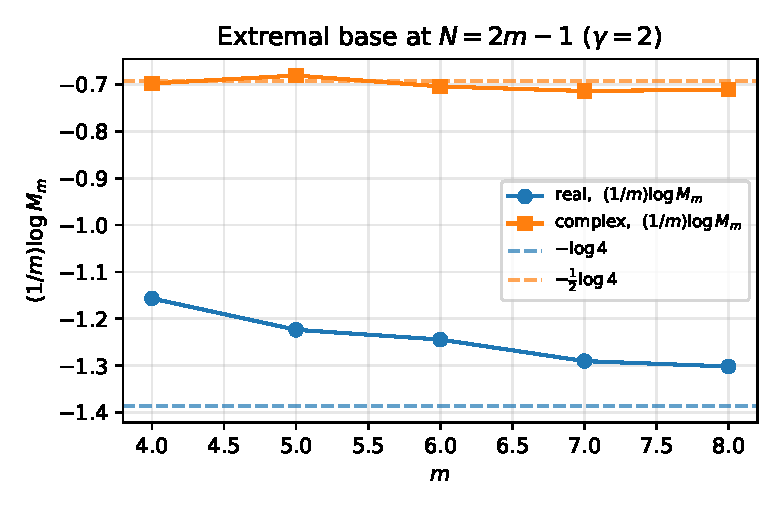
\includegraphics[width=.62\textwidth]{numerics/fig_base.pdf}
\caption{The extremal base $\tfrac1m\log M_m$ at $N=2m-1$ ($\gamma=2$), real and complex
Gaussian, by full enumeration of all $\binom{2m-1}{m}$ square row submatrices.  The values
approach the proved limits $-\log4$ (real) and $-\tfrac12\log4$ (complex).}
\label{fig:base}
\end{figure}

\begin{figure}[t]
\centering
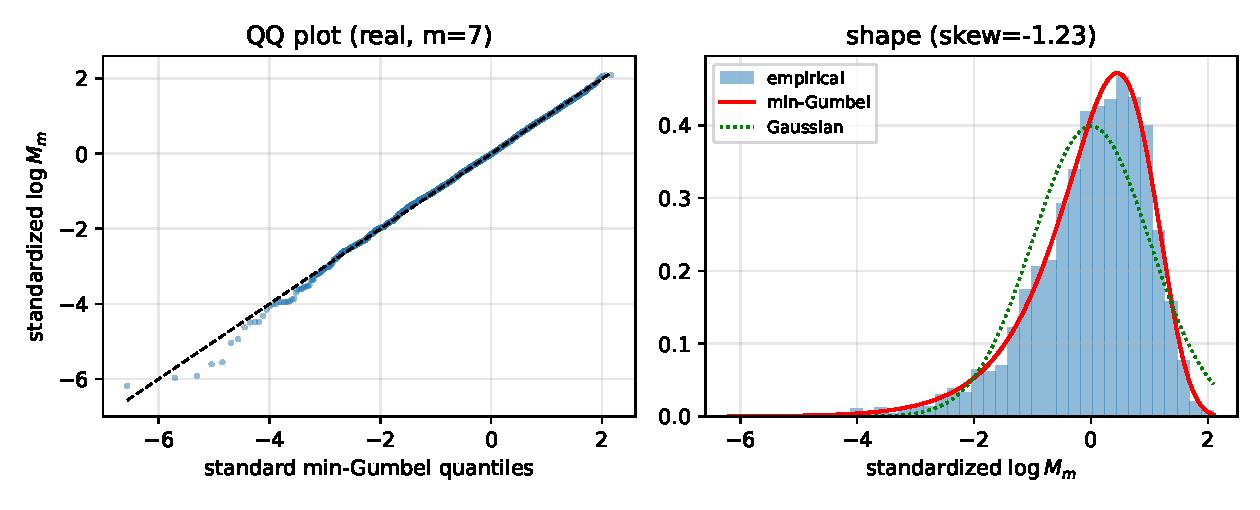
\includegraphics[width=.92\textwidth]{numerics/fig_gumbel.pdf}
\caption{Distribution of the standardized centered minimum $\log M_m$ (real, $m=7$,
$N=13$, $4000$ matrices).  Left: quantile--quantile plot against the reflected (minimum)
Gumbel law $1-e^{-e^{x}}$.  Right: histogram against the minimum-Gumbel density (red) and a
Gaussian (green, dotted).  The fit to the minimum Gumbel is excellent (Kolmogorov--Smirnov
statistic $0.008$, $p\approx0.96$; sample skewness $-1.23$), supporting the explicit
fluctuation law of Section~\ref{sec:open}; the Gaussian is plainly rejected.}
\label{fig:gumbel}
\end{figure}

The Kolmogorov--Smirnov test of the standardized $\log M_m$ against the minimum-Gumbel law
returns statistic $0.008$ with $p\approx0.96$ at $m=7$, so the conjectured limiting shape is
not rejected, while a Gaussian limit is decisively rejected by the skewness.

\paragraph{Rectangular and higher singular values.}
The geometric bases are confirmed by the same full-enumeration method (script
\texttt{numerics/verify\_geometric.py}, $\gamma=2$).  For the fixed-excess rectangular minimum
$M_m^{(r)}=\min_{|T|=m+r}\smin(A_T)$ the predicted base is $-h(2)/(d_\F(r+1))$: at $m=7$ the
empirical $\tfrac1m\log M_m^{(r)}$ is $-0.6935$ (real $r=1$, target $-0.6931$) and $-0.234$
(complex $r=2$, target $-0.231$), within a few thousandths.  For the $k$-th smallest singular
value $M_m[k]=\min_{|T|=m}\sigma_{m-k+1}(A_T)$ the predicted base is $-h(2)/(d_\F k^2)$: at
$m=7$ the empirical value is $-0.172$ (complex $k=2$, target $-0.173$) and $-0.697$ (complex
$k=1$, target $-0.693$), again essentially exact, and the $k^{-2}$ scaling ($/4$ at $k=2$,
$/9$ at $k=3$) is clearly visible.  These confirm the rectangular exponent $d_\F(r+1)$ and the
Laguerre repulsion exponent $d_\F k^2$.

\paragraph{Atomic obstruction.}
The nonzero-alphabet quotient specialization of the deterministic finite-alphabet
obstruction (Section~\ref{sec:atomic}) is also borne out:
for $S=\{\pm1\}$ ($q=2$), $S=\{1,2\}$ ($q=3$), and $S=\{1,2,4\}$ ($q=5$), every sampled
$A\in S^{N\times m}$ at the threshold $N=q(m-1)+1$ has a singular $m$-row submatrix (empirical
frequency $1.000$ across $m=2,3,4$ and $400$ matrices each), while just below the threshold the
frequency drops below one for small $m$ (e.g.\ $0.49$ for $\{\pm1\}$ at $m=2$, $N=2$), so
full-spark \(S\)-frames are seen in the sampled small cases.  This illustrates
the quotient pigeonhole obstruction without claiming an exhaustive sharpness
classification below the deterministic row count.

\paragraph{Two-sided submatrices.}
For the two-sided minimum $M=\min_{|R|=|C|=k}\smin(A_{R,C})$ at square aspect
$\gamma_R=\gamma_C=2$ ($N=n=2k$, real), where the entropy adds and the predicted base is
$-(h(2)+h(2))=-2\log4=-2.7726$, full enumeration over both row- and column-subsets gives
empirical $\tfrac1k\log M$ of $-2.32,-2.37,-2.56,-2.54$ for $k=3,\dots,6$, trending toward the
target and roughly double the one-sided value $-\log4$, confirming the entropy-addition
mechanism of Section~\ref{sec:geometric}.

\paragraph{Quaternion base (end to end).}
The quaternion exact law (Theorem~\ref{thm:quaternion-gaussian-base}) is confirmed directly, not
only through its overlap-moment ingredient.  Realifying each quaternion submatrix
($\HH^{m\times m}\hookrightarrow\R^{4m\times4m}$, so $\smin$ is preserved) and enumerating all
$\binom{2m}{m}$ square row submatrices of a standard quaternion Gaussian $A\in\HH^{2m\times m}$
($\gamma=2$, target $-h(2)/4=-0.3466$, script \texttt{numerics/verify\_quaternion.py}), the
empirical $\tfrac1m\log M_m$ is $-0.51,-0.48,-0.49,-0.46$ for $m=3,4,5,6$, with the gap to the
target shrinking ($-0.16,-0.13,-0.14,-0.11$); the value sits between the complex base
($-0.69$) and $0$, the correct ordering for $d_\HH=4$, and the fluctuation scale
($\approx\pi/(4\sqrt6)$) matches.  This validates the division-algebra base $-h(\gamma)/d_\F$
across $d_\F=1,2,4$.


\section{Open problems}\label{sec:open}
\begin{problem}[Second-moment universality: completing the self-contained estimate]\label{prob:pc}
Proposition~\ref{appB:resolvent} with Remark~\ref{appB:selfcontained} establishes the pair-correlation
condition for iid bounded-density entries self-contained --- an elementary off-support leave-one-out
estimate, with the anisotropic local law \cite{BEKYY2014,KnowlesYin2017} an optional citation ---
modulo routine error bookkeeping.  The problem here is to complete that bookkeeping with explicit
constants, to obtain the sharp rate \(M(D)=1+d_\F/(2D)+O(D^{-2})\), and to extend beyond bounded
density (general sub-Gaussian or atomic entries, where the marginal small-ball is more delicate).  By
Lemma~\ref{lem:two-proj} (two-projection local central limit theorem) and
Proposition~\ref{prop:small-D-negligible} (small/intermediate-codimension
negligibility), the upper side reduces to the bulk overlap-moment estimate, for
some fixed \(\varepsilon>0\),
\[
  \EE\!\left[(1-|\varrho_{I,J}|^2)^{-d_\F/2}\ ;\ D(I,J)\ge\varepsilon m\right]\le 1+o(1),
\]
where $\varrho_{I,J}=\langle u_I,u_J\rangle$ is the overlap of the unit normals of two
random $(m-1)$-row spans and $D(I,J)=m-|I\cap J|$.  This reduces further.  In the
shared orthocomplement $E^\perp\cong\F^D$ the normal $u$ is the null vector of
$D-1$ projected rows, and a polar-cap net/small-ball bound (Rudelson--Vershynin
invertibility) gives the lower tail
\(\PP\{1-|\varrho|^2\le y\}\le (C\sqrt y)^{D-1}+e^{-cD}\); with Markov this reduces
the moment to the single \emph{decorrelation} estimate
\[
  \EE|\varrho_{I,J}|^2=o(1)\qquad\Longleftrightarrow\qquad
  \sup_{\|w\|=1}\EE\big[|\langle u,w\rangle|^2\mid E\big]=o(1)\quad(D\to\infty),
\]
a delocalization in expectation of the random normal; this condition on
$\EE|\varrho|^2$ is both \emph{sufficient and necessary} for the displayed bound.  For
\emph{disjoint} row sets it is exact, $\EE|\varrho|^2=1/m$, because the signed-permutation/phase
symmetry of the iid law forces $\EE[uu^*]=I_m/m$.  For \emph{overlapping} sets it is the remaining
point: conditional isotropy of the projected rows pins only the trace of $\EE[uu^*\mid E]$, not its
spectrum, so a soft central-limit argument does not suffice.  The estimate is not obstructed,
however --- it holds with the sharp rate $\EE|\varrho|^2=(1+o(1))/D$ in every simulation we ran
(distribution-free, including non-symmetric bounded-density laws), and the apparent isotropic
obstruction with $\lambda_{\max}\asymp1$ is a fixed-small-dimension artifact whose top eigenvalue in
fact decays like $1/D$.  What remains is a no-gaps delocalization in expectation for the null vector
of projections of iid rows.  In the keystone's realization the projected rows are $g_i=B^*a_i$, so
$GG^*=B^*(AA^*)B$ is a deformed sample-covariance matrix and the estimate is a hard-edge,
direction-uniform delocalization of its bottom null vector at aspect ratio tending to one --- exactly
the object controlled by the anisotropic local law \cite{KnowlesYin2017,BEKYY2014}, whose adaptation to
this null-vector form (with the $E^\perp$ intersection constraint) would close the universality upper
side, and with it the fluctuation law of Conjecture~\ref{conj:gumbel}.  An Efron--Stein reduction
sharpens the target to the single-step increment $q_r-q_{r-1}=o(1/m)$ of the conditional overlap
moment $q_r=\EE[|\varrho|^2\mid |I\cap J|=r]$.
\end{problem}

\begin{conjecture}[Poisson hard-edge extreme process]\label{conj:gumbel}
Let \(A_m\in\F^{N_m\times m}\) be iid Gaussian with \(N_m/m\to\gamma>1\), and
let \(G_m\in\F^{m\times m}\) be one square Gaussian matrix.  Define \(b_m\) by
\[
  \binom{N_m}{m}F_m(e^{-b_m})=1,\qquad
  F_m(t)=\PP\{\smin(G_m)\le t\}.
\]
Prove that
\[
  \sum_{|T|=m}\delta_{\log\smin(A_{m,T})+b_m}
\]
converges to the Poisson extreme process with the hard-edge intensity.  This
would determine the \(\log m\) correction, the \(O(1)\) centering, and the
Gumbel law for \(\log M_m^\F\).
\end{conjecture}

\paragraph{Known first-moment part.}
The centering above is well-defined for all large \(m\), since \(F_m\) is
continuous, \(F_m(0)=0\), and \(F_m(t)\to1\).  Lemma~\ref{ldp:one-matrix} gives
\[
  b_m=\frac1{d_\F}\log\binom{N_m}{m}+O_\F(\log m)
      =\frac{h(\gamma)}{d_\F}m+o(m).
\]
If \(N_m=\gamma m+O(1)\), the exact Gaussian hard-edge formulas give the sharper
centering
\[
  b_m=
  \begin{cases}
    h(\gamma)m+O(1),& \F=\R,\\[2mm]
    \frac{h(\gamma)}2m+\frac14\log m+O(1),& \F=\C.
  \end{cases}
\]
Here the complex formula uses \(F_m(t)=1-e^{-mt^2}\), while the real formula
uses Edelman's finite-\(m\) hard-edge coefficient
\(\kappa_m=\sqrt2\,\Gamma((m+1)/2)/\Gamma(m/2)=m^{1/2}(1+O(m^{-1}))\)
\cite{Edelman1988}.

For fixed \(x\in\R\), put
\[
  Z_m^{\rm fl}(x)=
  \#\{T\subset[N_m]: |T|=m,\ \log\smin(A_{m,T})+b_m\le x\}.
\]
Then exactly
\[
  \EE Z_m^{\rm fl}(x)
  =
  \binom{N_m}{m}F_m(e^{x-b_m})
  =
  \frac{F_m(e^x e^{-b_m})}{F_m(e^{-b_m})}.
\]
The finite-\(m\) Gaussian hard-edge formulas imply, uniformly for fixed \(x\),
\[
  \frac{F_m(e^x e^{-b_m})}{F_m(e^{-b_m})}
  \longrightarrow e^{d_\F x}.
\]
Thus the conjectured point process has the correct first intensity:
\[
  \EE Z_m^{\rm fl}(x)\to e^{d_\F x},
\]
corresponding to the intensity measure \(d_\F e^{d_\F x}\,dx\).  Markov's
inequality gives the one-sided bound
\[
  \limsup_{m\to\infty}
  \PP\{\log M_m^\F+b_m\le x\}\le e^{d_\F x}.
\]
Using only the polynomial two-sided bound of Lemma~\ref{ldp:one-matrix}, without
the finite-\(m\) regular variation formula, one still has
\[
  \PP\{\log M_m^\F+b_m\le x\}
  \le C_\F m^{1+d_\F/2}e^{d_\F x},
\]
so
\[
  \PP\{\log M_m^\F+b_m\le-r_m\}\to0
  \qquad
  \text{whenever}\quad
  r_m-\frac{1+d_\F/2}{d_\F}\log m\to+\infty .
\]

If the point process in Conjecture~\ref{conj:gumbel} converges, then
\[
  \PP\{\log M_m^\F+b_m\le x\}
  \to 1-\exp(-e^{d_\F x}).
\]
Equivalently,
\[
  \PP\{-(\log M_m^\F+b_m)\le x\}\to \exp(-e^{-d_\F x}),
\]
the standard Gumbel form with rate \(d_\F\).

\paragraph{Critical Poisson overlap condition.}
The method of moments shows that Conjecture~\ref{conj:gumbel} would follow from
factorial moment convergence at the centered scale.  For every fixed
\(r\ge2\) and \(x_1,\ldots,x_r\in\R\), with
\(\tau_i=e^{x_i-b_m}\), one sufficient condition is
\[
  \sum_{\substack{(T_1,\ldots,T_r)\\\text{distinct}}}
  \PP\{\smin(A_{m,T_i})\le\tau_i,\ 1\le i\le r\}
  \longrightarrow
  \prod_{i=1}^r e^{d_\F x_i}.
\]
This is stronger than Problem~\ref{prob:pc}.  The latter is a bulk two-point
condition for the exponential-scale second-moment argument below the critical
line.  At the centered scale, the single-event probability is of order
\(\binom{N_m}{m}^{-1}\) up to polynomial factors, so the
small/intermediate-overlap range is no longer removed by
Proposition~\ref{prop:small-D-negligible}.  It does \emph{not}, however, require a
separate higher-order independence input.  The joint density of the \(r\) slabs is
governed by the Gram matrix \(G_r=(\langle u_{T_i},u_{T_j}\rangle)_{i,j}\) of the
\(r\) unit normals, and Gershgorin's bound
\(\lambda_{\min}(G_r)\ge 1-(r-1)\max_{i\ne j}|\varrho_{ij}|\) forces
\(\det G_r\to1\) on spread tuples from the \emph{pairwise} overlaps alone; the
higher-order asymptotic independence is thus a corollary of the two-point
statement, and a Chen--Stein/Arratia--Goldstein--Gordon argument collapses the
factorial moments to two-point terms, with no genuine \(r\)-point obstruction for
\(r\ge3\).  What remains is a single \emph{critical-scale} two-point estimate, with
a genuine subtlety at the minimal codimension.  For \(D(I,J)=2\) (row sets
differing in one index) the overlap obeys \(1-|\varrho|^2\sim\mathrm{Beta}(d_\F/2,d_\F/2)\),
so \(\EE[(1-|\varrho|^2)^{-d_\F/2}\mid D{=}2]=\infty\): no uniform moment bound
holds.  That divergence is the near-diagonal regime \(|\varrho|\to1\), where the two
least-singular-value events nearly coincide and the \emph{true} joint probability
is regularized to the first-moment scale \(p_1\) (a self-pairing term), not the
divergent local-CLT moment.  The required estimate is therefore the critical-scale
negligibility of the genuine \emph{off-diagonal} clustering,
\(\sum_{D\ge3}\#\{\text{codim-}D\text{ pairs}\}\,p_1^2\,M(D)\to0\) with
\(M(D)=\EE[(1-|\varrho|^2)^{-d_\F/2}\mid D]\) finite and \(\to1\) for \(D\ge3\),
together with the correct accounting of the \(D=2\) near-diagonal term --- the
regime Proposition~\ref{prop:small-D-negligible} no longer controls at the centered
scale.  For the Gaussian ensemble the overlap is exactly
\(|\varrho|^2\sim\operatorname{Beta}(d_\F/2,d_\F(D-1)/2)\), giving the closed form
\[
  M(D)=\frac{\Gamma\!\big(\tfrac{d_\F(D-2)}2\big)\,\Gamma\!\big(\tfrac{d_\F D}2\big)}
            {\Gamma\!\big(\tfrac{d_\F(D-1)}2\big)^2}
       =1+\frac{d_\F}{2D}+O(D^{-2})\qquad(D\ge3),
\]
so the association constant \(C(D)=M(D)\) is explicit, bounded, and summable against
the polynomial codimension counts; the Gaussian case of the bounded-association bound
is thus a finite computation, and the keystone (Problem~\ref{prob:pc}) is exactly the
statement that \(M(D)\) retains this value universally.

For the Gaussian ensemble the reduction is \emph{exact}.  Conditioning on the shared rows makes the two
events $\{\smin(A_S)\le t_m\}$, $\{\smin(A_T)\le t_m\}$ conditionally i.i.d., so with
\(q=\PP\{\smin(A_T)\le t_m\mid A_S\}\) and the hypergeometric (Vandermonde) codimension law \(P_{\mathrm V}(D)\),
\[
  \EE[(N_t)_2]=\Big(\tbinom Nm\,p_1\Big)^2\sum_{D\ge2}P_{\mathrm V}(D)\,M_m(D),\qquad
  M_m(D):=\frac{\EE[q^2]}{(\EE q)^2}\ge1,
\]
and the Gumbel law is \emph{equivalent} to \(\EE_{\mathrm V}[M_m(D)]\to1\).  On the bulk \(D\ge\varepsilon m\)
this is rigorous: rotational invariance makes the two null directions Haar in the shared orthocomplement,
so \(|\varrho|^2\sim\operatorname{Beta}(d_\F/2,d_\F(D-1)/2)\) \emph{exactly} and
\(M_m(D)\le(1+o(1))M(D)=1+d_\F/(2D)+O(D^{-2})=1+O(1/m)\), the rare \(|\varrho|\to1\) killed by the
super-exponential Beta tail.  The lone residual is a uniform polynomial bound \(M_m(D)\le\mathrm{poly}(m)\)
for the small codimensions \(1\le D<\varepsilon m\) at the \emph{centered} scale, where the two-projection
expansion is void; the worst case is \(M_m(1)=\Theta(m)\) (a centered-scale \(\log(1/t_m)=\Theta(m)\)
effect, invisible to moderate-scale simulation), which is polynomial, so the exponentially light
\(P_{\mathrm V}(D<\varepsilon m)=e^{-\Theta(m)}\) removes it.  This is the fluctuation-law analogue of the
keystone reduction: the universality base reduces to one overlap estimate, the Gaussian Gumbel law to a
uniform small-codimension hard-edge bound.

Simulation indicates the limit is \emph{simple} Poisson, so no compound (cluster)
correction to the Gumbel law is needed.  At the \(2\%\)--\(5\%\) lower quantile the
\(D=2\) co-occurrence ratio \(\PP\{\text{both small}\}/\PP\{\text{small}\}^2\) is
\(4\)--\(7\), with conditional \(\PP\{T\text{ small}\mid S\text{ small}\}\approx0.13\)--\(0.20\)
\emph{decreasing} toward the extremal scale, while large-\(D\) pairs are independent
(ratio \(\approx1\)); the association of the closest pairs is bounded, not divergent.
Since each submatrix has only \(O(m^2)\) codimension-\(2\) neighbours against
\(\binom{N}{m}\) submatrices in all, their total contribution to \(\EE[(N_t)_2]\) is
\(O\!\big(m^2/\binom{N}{m}\big)\lambda^2\to0\), and the exponentially many independent
large-\(D\) pairs supply the \(\lambda^2\).  Thus the extremal index is one, reducing
Conjecture~\ref{conj:gumbel} to a rigorous version of this count: a centred-scale
bounded-association bound \(\PP\{\text{both}\mid D\}\le C(D)\,p_1^2\) with summable
polynomial codimension weights.  Directly, full enumeration of all \(\binom{N}{m}\)
submatrices (calibrated to \(\EE N_t=\lambda=2\)) gives the second factorial-moment
ratio \(\EE[N_t(N_t-1)]/(\EE N_t)^2=1.18,1.13,1.04\) for \(m=6,7,8\), decreasing to
the Poisson value \(1\), with \(\operatorname{Var}(N_t)/\EE N_t=1.37,1.25,1.07\) and
\(\PP\{N_t=0\}=0.157,0.157,0.139\to e^{-\lambda}=0.135\): the simple-Poisson signature
sharpens with \(m\) as the finite-size small-codimension excess decays.

\begin{problem}[Hard-edge avoidance speed]\label{prob:avoidance}
For the Gaussian square-row-submatrix model and \(s<h(\gamma)/d_\F\), determine
whether
\[
  \lim_{m\to\infty}\frac1m
  \log\!\left[-\log\PP\left\{
  \min_{|T|=m}\smin(A_T)>e^{-sm}
  \right\}\right]
  =h(\gamma)-d_\F s.
\]
If this equality fails, identify the overlap-cluster correction.  This is the
dependent avoidance counterpart to the easy union-bound tail
\[
  \PP\{M_m\le e^{-sm}\}\le \exp((h(\gamma)-d_\F s+o(1))m)
\]
for \(s>h(\gamma)/d_\F\).
\end{problem}

\begin{problem}[Atomic full spark beyond the sign obstruction]\label{prob:atomic-fullspark}
For a specified atomic class, such as Bernoulli-\(p\) entries or bounded-support
integer-valued entries, determine the threshold below the available deterministic
projective-pair obstruction row counts at which some \(m\times m\) row
submatrix is singular with high probability.  Proposition~\ref{prop:sign-critical}
is the symmetric sign case of the finite-alphabet projective-pair obstruction,
but below such deterministic row counts general atomic laws have law-dependent
collision and inverse Littlewood--Offord structure.
\end{problem}

\begin{problem}[Log-concave extremal hard edge]\label{prob:logconcave}
For iid isotropic log-concave rows, prove the matching upper side, or disprove
it, for the square and fixed-excess lower-side bases:
\[
  \frac1m\log\min_{|T|=m}\smin(A_T)\stackrel{?}{\longrightarrow}-h(\gamma),
  \qquad
  \frac1m\log M_m^{(r)}\stackrel{?}{\longrightarrow}
  -\frac{h(\gamma)}{r+1}.
\]
The lower sides follow from directional anti-concentration; the open input is
the pair-correlation theorem for dependent-coordinate rows.
\end{problem}

\begin{problem}[Frame-design optimization]\label{prob:frame-design}
Among iid continuous real row ensembles at \(N=2m-1\) with isotropy
\(\EE aa^T=I_m\), bounded row-norm moments, and uniformly bounded one-dimensional
densities, determine which laws minimize or maximize the Balan--Wang exponential
base.  The problem should specify whether rows are normalized to the sphere or
allowed to have exponential radial extremes; subexponential radial variation is
covered by Theorem~\ref{thm:rot-inv-univ} and does not change the base.
\end{problem}

\begin{problem}[Complex stability base]\label{prob:complex-pr}
At the generic \(4m-4\) complex phase-retrieval threshold, determine the exponential base for the
complex Balan--Wang stability constant
\[
  a(\Phi)=\inf_{x\not\sim e^{i\theta}y}
  \frac{\||Ax|-|Ay|\|}{\dist(x,\mathbb T y)}
  =\min_{\substack{S=S^*,\ \rank S\le2,\ S\ne0}}
  \frac{\|(\phi_i^*S\phi_i)_{i=1}^N\|}{\|S\|},
\]
the second equality because \(xx^*-yy^*\) is Hermitian of rank \(\le2\).  The rank-\(\le2\) Hermitian
cone has real dimension \(2(2m-2)=4m-4\), matching the threshold \(N\), so
\(S\mapsto(\phi_i^*S\phi_i)\) is a \emph{square} sensing map and \(a(\Phi)\) is its extremal hard edge
--- the exact analogue of the real case (cone dimension \(2m-1=N\)).  Two ingredients differ from the
real frame.  \emph{Small-ball (here proved):} for the signature-\((1,1)\) perturbations
\(S=xx^*-yy^*\), \(\phi_i^*S\phi_i=\lambda_1|\langle\phi_i,e_1\rangle|^2-\lambda_2|\langle\phi_i,e_2\rangle|^2\)
is a difference of two independent exponentials with strictly positive density at the origin, so
\(\PP\{|\phi_i^*S\phi_i|\le t\}\asymp t\) with exponent \(1\) --- \emph{not} the naive complex value
\(d_\C=2\), since an indefinite quadratic form crosses zero transversally.  \emph{Entropy:} the
realified configuration count is \(\tfrac1m\log\binom{4m-4}{2m-2}\to\log16\).  The principle of
Section~\ref{sec:principle} then predicts a finite \emph{candidate base}
\[
  a(\Phi)=c^{-m+o(m)}\qquad(\text{conjectured},\ c\ \text{finite}),
\]
with \(c=16\) (the square of the real base \(4^{-m}\)) suggested by the realification count
\(\binom{4m-4}{2m-2}\); the exact value is open, since the two-direction stratification below counts
\(\binom{N}{k}^2\) and admits \(c\) up to \(256\).  The lower side is partially settled.  The constant reduces
\emph{exactly} to a Grassmannian least-singular-value statistic,
\[
  a(\Phi)=\min_{U\in\mathrm{Gr}_\C(2,m)}\sigma_{\min}\big(M(U)\big),
\]
where \(M(U)\) is the \((4m-4)\times4\) real matrix of the evaluation
\(H\mapsto(w_i^*Hw_i)_i\), \(w_i=U^*\phi_i\), over \(2\times2\) Hermitian \(H\); and a first-moment/net
argument over this Grassmannian (real dimension \(4m-8\)), fed the exponent-\(1\) small-ball, proves the
sub-exponential bound
\[
  a(\Phi)\ \ge\ m^{-(2+o(1))m}\qquad\text{with high probability.}
\]
The gap to a finite base is the net's Lipschitz cost \(e^{\Theta(m\log m)}\):
closing it needs a Segre/bilinear least-singular-value small-ball (constant exponent, subexponential
constant) for \(\Re(\bar p_iq_i)\), which is irreducible (no exact finite combinatorial family as in
the real case).  That single estimate is the missing RMT input, and a net analysis shows it is
unavoidable: at the critical count every split of the \(N\)-dimensional sensing into netted and
exactly-treated coordinates leaves union-deficit one, while the eigenvectors enter
\(|\langle\phi_i,u\rangle|^2\) nonlinearly, so \(\Theta(m)\) directions must be netted and the
Lipschitz cost is paid \(\Theta(m)\) times.  The exponential decay is moreover a \emph{critical-point}
phenomenon: at \(N=(4+\eta)m\), \(\eta>0\), the same argument gives only the polynomial bound
\(a(\Phi)\ge m^{-2/\eta}\), so genuine exponential decay of the stability constant occurs precisely at
the injectivity threshold \(N=4m-4\).
\end{problem}

\begin{problem}[Proportional rectangular / sample-covariance edge]\label{prob:rectangular}
For \(\ell/m\to\zeta\in(1,\gamma)\), define
\[
  M_{m,\ell}=\min_{|T|=\ell}\smin(A_T)/\sqrt m.
\]
Equivalently,
\[
  \min_{|T|=\ell}
  \lambda_{\min}\!\left(\ell^{-1}A_T^*A_T\right)
  =\frac{m}{\ell}M_{m,\ell}^2 .
\]
Prove convergence of \(M_{m,\ell}\), and identify its limit through the
left-tail large-deviation rate \(I^-_{\zeta,d_\F}\) for the smallest rectangular
Wishart eigenvalue:
\[
  I^-_{\zeta,d_\F}(x_{\gamma,\zeta})=
  \gamma\log\gamma-\zeta\log\zeta-(\gamma-\zeta)\log(\gamma-\zeta).
\]
The fixed-excess formula \(-h(\gamma)/(d_\F(r+1))\) does not apply in this
regime.
\end{problem}

\begin{problem}[Trimmed projection concentration]\label{prob:trimmed}
For iid isotropic rows \(a_i\), develop sharp concentration and large
deviations for
\[
  \inf_{\|x\|=1}\sum_{i=1}^{\lfloor N/2\rfloor}
  \bigl(\langle a_i,x\rangle^2\bigr)_{(i)},
\]
where the order statistics are increasing.  This statistic is the fixed-split
analogue of the worst half-frame conditioning problem in phase retrieval.
\end{problem}

\begin{problem}[Smoothed bad frames]\label{prob:smoothed}
Let \(F_m\in\R^{N_m\times m}\), \(N_m/m\to\gamma>1\), be a deterministic frame
with normalized row norms and poor extremal row-submatrix conditioning.  Put
\(A_m=F_m+\sigma_m G_m\), where \(G_m\) is Gaussian.  Determine the threshold
scale of \(\sigma_m\) at which
\[
  \min_{|T|=m}\smin((A_m)_T)
\]
recovers the Gaussian exponential scale.  The answer should depend on the
worst deterministic row-submatrix deficiency of \(F_m\).
\end{problem}

\begin{problem}[Exponential radial extremes]\label{prob:radial-mixture}
Theorem~\ref{thm:rot-inv-univ} shows that spherical row directions with
subexponential global radial variation have the same base as the Gaussian
row-submatrix model, up to the deterministic radial scale.  Determine the sharp
base when the sampled radii themselves have exponential extremes: for instance,
when the empirical lower tail of
\[
  m^{-1}\log(R_{im}/b_m)
\]
has a nontrivial large-deviation rate among the \(N_m\asymp m\) available rows.
The answer should combine the hard-edge entropy \(h(\gamma)\) with a weighted
selection problem for the row radii, rather than only the worst global
diagonal-sandwich bound.
\end{problem}


\appendix
\section{Proof of the two-projection anti-concentration lemma}\label{sec:app-two-proj}
% Appendix: full proof of Lemma lem:two-proj (two-projection anti-concentration).
% Real case in full; the complex case is identical with d_F=2. Uses manuscript macros and \varrho.

We give the complete proof of Lemma~\ref{lem:two-proj}.  Throughout $\F=\R$ (the complex case is
identical with $d_\F=2$, replacing each slab by a disk and $\sqrt{1-\varrho^2}$ by $1-|\varrho|^2$).
Recall $x\in\R^m$ has i.i.d.\ entries with mean $0$, variance $1$, density $f\le K$; $u,v$ are
deterministic unit vectors with $\|u\|_\infty,\|v\|_\infty\le\beta:=m^{-1/2+\delta}$,
$\varrho=\langle u,v\rangle$, $|\varrho|\le1-\kappa_0$; and $S_1=\langle x,u\rangle$,
$S_2=\langle x,v\rangle$, with $p(t)=\PP\{|S_1|\le t\}$, $q(t)=\PP\{|S_1|\le t,|S_2|\le t\}$.

Let $\psi(\theta)=\EE e^{i\theta x_1}$ denote the (common) entry characteristic function.

\begin{lemma}[Characteristic-function bound]\label{app:cf}
There are constants $\eta>0$ and $C_\psi<\infty$, depending only on the entry law, with
\[
  |\psi(\theta)|\le e^{-\eta\min(\theta^2,1)}\quad(\theta\in\R),
  \qquad \|\psi\|_{L^2(\R)}^2=2\pi\!\int f^2\le 2\pi K=:C_\psi .
\]
\end{lemma}
\begin{proof}
Let $x_1'$ be an independent copy and $Y=x_1-x_1'$, so $\EE Y^2=2$ and
$|\psi(\theta)|^2=\EE\cos(\theta Y)$.  From $1-\cos s\ge\tfrac14 s^2$ for $|s|\le1$, choosing
$\theta_0\in(0,1]$ with $\EE[Y^2\mathbf 1_{|Y|>1/\theta_0}]\le1$ gives, for $|\theta|\le\theta_0$,
$1-|\psi(\theta)|^2\ge\tfrac14\theta^2\,\EE[Y^2\mathbf 1_{|\theta Y|\le1}]\ge\tfrac14\theta^2$,
so $|\psi(\theta)|\le e^{-\theta^2/8}$ (only finite variance is used).  Since $f$ is a density,
$x_1$ is non-lattice, $|\psi|<1$ off $0$, and $\psi\to0$ at infinity (Riemann--Lebesgue), so
$\kappa:=\sup_{|\theta|\ge\theta_0}|\psi|<1$.  Taking $\eta=\min\{\tfrac18,\log(1/\kappa)\}$ gives
the pointwise bound on the three ranges $|\theta|\le\theta_0$, $\theta_0\le|\theta|\le1$,
$|\theta|\ge1$.  Plancherel gives $\|\psi\|_2^2=2\pi\int f^2\le2\pi K$.
\end{proof}

Set $w_j=(u_j,v_j)\in\R^2$ and $c_j(\xi)=\langle\xi,w_j\rangle$ for $\xi\in\R^2$, so that
$\xi_1S_1+\xi_2S_2=\sum_jc_j(\xi)x_j$ and, since $\|u\|=\|v\|=1$, $\langle u,v\rangle=\varrho$,
\begin{equation}\label{app:frame}
  \sum_{j}w_jw_j^{\top}=\Sigma:=\begin{pmatrix}1&\varrho\\\varrho&1\end{pmatrix},\quad
  \sum_j c_j(\xi)^2=\xi^\top\Sigma\xi\ge\kappa_0|\xi|^2,\quad
  |c_j(\xi)|\le\sqrt2\,\beta|\xi|,
\end{equation}
using $\lambda_{\min}(\Sigma)=1-|\varrho|\ge\kappa_0$ and $\det\Sigma=1-\varrho^2\ge\kappa_0$.
The joint characteristic function factorizes as $\phi_m(\xi)=\prod_j\psi(c_j(\xi))$, and the
target Gaussian has $\widehat{\Gamma_\Sigma}(\xi)=e^{-\frac12\xi^\top\Sigma\xi}$.

\begin{lemma}[Transverse pairs and integrability]\label{app:transverse}
For $m$ large there are two disjoint index pairs $\{p_i,q_i\}$ ($i=1,2$) with
$|\det[w_{p_i}\,|\,w_{q_i}]|\ge\Delta:=\sqrt{\kappa_0}/m$.  Consequently $\phi_m\in L^1(\R^2)$ with
$\int_{\R^2}|\phi_m|\le \|\psi\|_2^4/\Delta\le m\,C_\psi^2/\sqrt{\kappa_0}$.
\end{lemma}
\begin{proof}
With $W=[w_1\,|\cdots|\,w_m]$, Cauchy--Binet gives $\sum_{p<q}\det[w_p|w_q]^2=\det(WW^\top)=
\det\Sigma\ge\kappa_0$; as there are $<m^2/2$ pairs, some pair has $|\det|\ge\sqrt{2\kappa_0}/m$.
Removing it changes $\Sigma$ by $\le4\beta^2$ in operator norm, leaving determinant
$\ge\kappa_0/2$, so a second disjoint pair exists with $|\det|\ge\sqrt{\kappa_0}/m$.  Bounding the
other $m-4$ factors of $|\phi_m|$ by $1$, Cauchy--Schwarz over the two pairs and the linear change
of variables $\xi\mapsto(c_{p_i},c_{q_i})$ (Jacobian $\ge\Delta$) with Lemma~\ref{app:cf} give
$\int|\phi_m|\le\prod_{i=1,2}(\int|\psi(c_{p_i})\psi(c_{q_i})|^2)^{1/2}\le\|\psi\|_2^4/\Delta$.
\end{proof}

\begin{lemma}[Energy bound]\label{app:energy}
$F(\xi):=\sum_j\min(c_j(\xi)^2,1)\ge\tfrac{\kappa_0}{4}\min(|\xi|^2,\beta^{-2})$, hence by
Lemma~\ref{app:cf}, $|\phi_m(\xi)|\le\exp\{-\tfrac{\eta\kappa_0}{4}\min(|\xi|^2,\beta^{-2})\}$.
\end{lemma}
\begin{proof}
If $|\xi|\le(\sqrt2\beta)^{-1}$ then all $|c_j|\le1$ and $F=\sum c_j^2\ge\kappa_0|\xi|^2$.  If
$|\xi|>(\sqrt2\beta)^{-1}$, split into $\mathcal B=\{|c_j|>1\}$ and its complement.  If
$|\mathcal B|\ge\tfrac{\kappa_0}4\beta^{-2}$ then $F\ge|\mathcal B|\ge\tfrac{\kappa_0}4\beta^{-2}$;
otherwise $\sum_{j\notin\mathcal B}c_j^2\ge\xi^\top\Sigma\xi-|\mathcal B|\,2\beta^2|\xi|^2\ge
\tfrac{\kappa_0}2|\xi|^2>\tfrac{\kappa_0}4\beta^{-2}$.  In all cases $F\ge\tfrac{\kappa_0}4\min(|\xi|^2,\beta^{-2})$.
\end{proof}

\begin{proposition}[Local CLT]\label{app:lclt}
$(S_1,S_2)$ has a bounded continuous density $g_m$, and
$\varepsilon_m:=\sup_w|g_m(w)-\Gamma_\Sigma(w)|\le(2\pi)^{-2}\int_{\R^2}|\phi_m-\widehat{\Gamma_\Sigma}|\to0$,
uniformly over delocalized unit $u,v$ with $|\varrho|\le1-\kappa_0$.
\end{proposition}
\begin{proof}
$\phi_m\in L^1$ (Lemma~\ref{app:transverse}) and $\widehat{\Gamma_\Sigma}\in L^1$
($\det\Sigma\ge\kappa_0$) justify Fourier inversion and the displayed bound.  Fix $\varepsilon>0$
and split $\int|\phi_m-\widehat{\Gamma_\Sigma}|$ over $|\xi|\le R$, $R<|\xi|\le\beta^{-1}$,
$|\xi|>\beta^{-1}$.  Choose $R=R(\kappa_0,\varepsilon)$ with
$\int_{|\xi|>R}e^{-\kappa_0|\xi|^2/2}\le\varepsilon$.
\emph{(I) $|\xi|\le R$:} since $\max_j|c_j|\le\sqrt2\beta R\to0$, the expansion
$\psi(\theta)=1-\tfrac12\theta^2+\theta^2\omega(|\theta|)$ ($\omega\to0$) gives
$\log\phi_m(\xi)=-\tfrac12\xi^\top\Sigma\xi+E_m(\xi)$ with $|E_m|\le\omega^*(\sqrt2\beta R)\,
\xi^\top\Sigma\xi\le2R^2\omega^*(\sqrt2\beta R)\to0$; hence the integrand $\to0$ uniformly on the
ball and term I $\to0$.  \emph{(II) $R<|\xi|\le\beta^{-1}$:} here $\min(|\xi|^2,\beta^{-2})=|\xi|^2$,
so by Lemma~\ref{app:energy} the integrand is $\le e^{-\frac{\eta\kappa_0}4|\xi|^2}+
e^{-\frac{\kappa_0}2|\xi|^2}$, with integral $\le\varepsilon$ for $R$ large.  \emph{(III)
$|\xi|>\beta^{-1}$:} the residual $m-4$ indices have $\lambda_{\min}\ge\kappa_0/2$, so
Lemma~\ref{app:energy} gives $\sum_{j\notin Q}\min(c_j^2,1)\ge\tfrac{\kappa_0}8\beta^{-2}$, and with
Lemma~\ref{app:transverse},
$\int_{|\xi|>\beta^{-1}}|\phi_m|\le e^{-\frac{\eta\kappa_0}8 m^{1-2\delta}} m C_\psi^2/\sqrt{\kappa_0}\to0$;
the Gaussian far tail $\to0$ likewise.  Thus $\limsup_m\int|\phi_m-\widehat{\Gamma_\Sigma}|\le2\varepsilon$.
\end{proof}

\begin{proof}[Proof of Lemma~\ref{lem:two-proj}]
The one-dimensional specialization of Proposition~\ref{app:lclt} (single form $S_1$, coefficients
$u_j$, integrability from the two largest coefficients $u_{(1)}^2\ge1/m$, $u_{(2)}^2\ge1/(2m)$)
gives $\varepsilon_m':=\sup_w|g_{1,m}(w)-\Gamma_1(w)|\to0$, where $\Gamma_1$ is the standard
Gaussian density and $g_{1,m}$ the density of $S_1$.  Write $V_t=2t$.  Since the Gaussian densities
peak at the origin, with $\Gamma_\Sigma(0)=\Gamma_1(0)^2/\sqrt{1-\varrho^2}$,
\[
  q(t)\le(\Gamma_\Sigma(0)+\varepsilon_m)V_t^2,\qquad
  p(t)\ge\bigl(\Gamma_1(0)(1-\tfrac12t^2)-\varepsilon_m'\bigr)V_t .
\]
As $|\varrho|\le1-\kappa_0$ keeps $\Gamma_\Sigma(0)\le\Gamma_1(0)^2\kappa_0^{-1/2}$ bounded, both
$\varepsilon_m/\Gamma_\Sigma(0)\to0$ and $\varepsilon_m'/\Gamma_1(0)\to0$ uniformly, so for $t\to0$
\[
  \frac{q(t)}{p(t)^2}\le\frac{(\Gamma_\Sigma(0)+\varepsilon_m)V_t^2}
       {(\Gamma_1(0)(1-\tfrac12t^2)-\varepsilon_m')^2V_t^2}
  =\frac{\Gamma_\Sigma(0)}{\Gamma_1(0)^2}(1+o(1))=\frac{1+o(1)}{\sqrt{1-\varrho^2}} .
\]
For $\F=\C$ the argument is the same with the following substitutions, all routine.
Coefficients $c_j(\xi)\in\C$ ($\xi\in\C^2$); the entry characteristic function is
$\psi(\theta)=\EE e^{i\Re(\bar\theta x_1)}$, and Lemma~\ref{app:cf} holds verbatim from
$\EE x_1=0$, $\EE|x_1|^2=1$ (properness $\EE x_1^2=0$ makes the quadratic term
$\tfrac12|\theta|^2$ isotropic) and the bounded $\R^2$-density, with
$\|\psi\|_{L^2(\R^2)}^2=(2\pi)^2\!\int f^2\le(2\pi)^2K$.  The frame lives in $\C^2\simeq\R^4$:
$w_j=(u_j,v_j)$, $\sum_j w_jw_j^{*}=\Sigma$, and Cauchy--Binet (now over the $4\times2m$ real form
of $W$) again yields two transverse pairs with $|\det|\gtrsim m^{-1}$, so $\phi_m\in L^1(\C^2)$.
The energy bound and three-region inversion are unchanged, giving
$\|g_m-\Gamma_\Sigma\|_\infty\to0$ for the proper complex Gaussian $\Gamma_\Sigma$ on $\C^2$ with
$\Gamma_\Sigma(0)=\Gamma_1(0)^2/(1-|\varrho|^2)$.  Converting with disks ($V_t=\pi t^2$,
$d_\F=2$) gives $q(t)\le(1+o(1))p(t)^2/(1-|\varrho|^2)$.
\end{proof}


\section{Reduction of the pair-correlation condition to one decorrelation estimate}\label{sec:app-keystone}
% Appendix B: the pair-correlation condition reduces to one decorrelation estimate.
% Promotes notes/keystone_{tail,assembly_bar,typical}.md into the manuscript. Real case in full;
% complex identical with d_F=2. Uses manuscript macros and \varrho.

Throughout, $A_m\in\F^{N_m\times m}$ has iid entries that are mean zero, unit variance, with a
symmetric (real) / circular (complex) law of bounded Lebesgue density $\le K$ and sub-Gaussian.
Fix the distinguished row $x=a_{N_m}$.  For an $(m-1)$-set $S$ let $u_S$ be a unit normal to
$\spn\{a_i:i\in S\}$; for $S\ne T$ with $|S\cap T|=m-D$ write $\varrho=\langle u_S,u_T\rangle$ for
their overlap and, conditioning on the shared rows, work in the $D$-dimensional orthocomplement
$E^\perp$ of their span, where $u_S,u_T$ are the unit null vectors of the $D-1$ projected disjoint
rows.  Put $X=1-|\varrho|^2\in(0,1]$ and $a=d_\F/2$.  The pair-correlation condition of
Section~\ref{sec:universality} requires $\Var Z_m(s)/(\EE Z_m(s))^2\to0$, which (after
Lemma~\ref{lem:two-proj} and Proposition~\ref{prop:small-D-negligible}) is the bulk overlap moment
$\EE[X^{-a};\,D\ge\varepsilon m]\le1+o(1)$.  We reduce this to a single decorrelation estimate.

\begin{lemma}[Polar-cap lower tail]\label{appB:tail}
There are $C,c>0$ depending only on $(K,\F)$ such that, for the null vector $u$ of $D-1$ iid
isotropic sub-Gaussian bounded-density vectors in $\F^D$ and any fixed unit $e\in\F^D$,
\[
  \PP\{\,|\langle e,u\rangle|^2\ge 1-y\,\}\le (C\sqrt y\,)^{\,d_\F(D-1)}+2e^{-cD},
  \qquad 0<y<1 ,
\]
\end{lemma}

\begin{proof}[Proof (real case; complex replaces $D-1$ by $2(D-1)$)]
Let $G=[g_1\,|\cdots|\,g_{D-1}]$ and $A=G^*$, so $u$ is the unit right-null vector of $A$, and
$\|A\|=\|G\|$.  For iid isotropic sub-Gaussian columns, the operator-norm bound
\cite{Vershynin2018} gives $\PP\{\|A\|>R\sqrt D\}\le2e^{-c_1R^2D}$ for $R\ge C_1(K)$.  The polar
cap $\mathrm{Cap}=\{v\in S^{D-1}:|\langle e,v\rangle|\ge\sqrt{1-y}\}$ has transverse radius
$\sin\theta=\sqrt y$, so it admits a $\delta$-net $\mathcal N$ with
$|\mathcal N|\le(C_0\sqrt y/\delta)^{D-1}$.  If $u\in\mathrm{Cap}$ and $\|A\|\le R\sqrt D$, choose
$z\in\mathcal N$ with $\|z-u\|\le\delta$; since $Au=0$, $\|Az\|=\|A(z-u)\|\le R\sqrt D\,\delta$.
Hence
\[
  \PP\{u\in\mathrm{Cap}\}\le 2e^{-c_1R^2D}+\sum_{z\in\mathcal N}\PP\{\|Az\|\le R\sqrt D\,\delta\}.
\]
For fixed unit $z$, $\|Az\|^2=\sum_{i=1}^{D-1}|\langle g_i,z\rangle|^2$ is a sum of $D-1$ iid
nonnegative variables with unit mean and marginal small-ball $\le Kr$ (bounded density); the
tensorized Laplace bound \cite{RudelsonVershynin2008} gives
$\PP\{\|Az\|^2\le R^2D\delta^2\}\le(C_2KR\delta)^{D-1}$.  Therefore
\[
  \PP\{u\in\mathrm{Cap}\}\le2e^{-c_1R^2D}+(C_0\sqrt y/\delta)^{D-1}(C_2KR\delta)^{D-1}
   =2e^{-c_1R^2D}+(C_0C_2KR\sqrt y\,)^{D-1};
\]
the $\delta$ cancels --- the cap's smallness $\sqrt y$ is exactly the per-coordinate small-ball
gain --- so no $\sqrt D$ factor survives.  Take $R=C_1$.
\end{proof}

\begin{proposition}[Assembly: the bar is $\EE|\varrho|^2=o(1)$]\label{appB:assembly}
Let $\mu_1=\EE|\varrho|^2=\EE[1-X]$.  Using Lemma~\ref{appB:tail} (tuned $R=y^{-1/4}$ for the
singular part),
\[
  \EE[X^{-a}]\le 1+O(\sqrt{\mu_1})+o(1),
\]
where $o(1)\to0$ as $D\to\infty$ uniformly.  In particular $\EE[X^{-a}]=1+o(1)$ if and only if
$\mu_1=o(1)$.
\end{proposition}

\begin{proof}
Split $\EE[X^{-a}]=\EE[X^{-a};X\le y_1]+\EE[X^{-a};y_1<X\le\tfrac12]+\EE[X^{-a};X>\tfrac12]$ with
$y_1$ a small constant.  (i) By Lemma~\ref{appB:tail}, $\EE[X^{-a};X\le y_1]\le\sum_{k\ge k_1}
2^{(k+1)a}\PP\{X\le2^{-k}\}=o(1)$, independent of $\mu_1$ (the geometric/tuned-tail series
converges).  (ii) Markov on $1-X$: $\PP\{X\le\tfrac12\}\le2\mu_1$, so
$\EE[X^{-a};y_1<X\le\tfrac12]\le y_1^{-a}\cdot2\mu_1=O(\mu_1)$.  (iii) On $X>\tfrac12$ write
$X^{-a}=1+(X^{-a}-1)$; splitting at $1-\eta$, the part $X>1-\eta$ has $X^{-a}-1\le C_a\eta$, and the
part $\tfrac12<X\le1-\eta$ has $X^{-a}-1\le2^a$ with $\PP\{X\le1-\eta\}\le\mu_1/\eta$, so
$\EE[X^{-a};X>\tfrac12]\le1+C_a\eta+2^a\mu_1/\eta$.  Optimizing $\eta=\sqrt{\mu_1}$ gives
$1+O(\sqrt{\mu_1})$.  Summing the three parts gives the claim; necessity follows from
$\EE[X^{-a}]\ge\EE[1+aX^{-1}(1-X)]\ge1+a\mu_1$ via $(1-t)^{-a}\ge1+at$.
\end{proof}

\begin{proposition}[Exact decorrelation for disjoint sets]\label{appB:disjoint}
For every $(m-1)$-set $S$, $\EE[u_Su_S^*]=\tfrac1m I_m$.  Consequently, for disjoint $S,T$,
$\EE|\varrho|^2=\tfrac1m$.
\end{proposition}

\begin{proof}
The iid entry law is invariant under coordinate permutations $\pi$ and under sign flips (real) /
coordinate phase rotations (complex); the normal direction is equivariant, $u_{S}\mapsto P_\pi u_S$
resp.\ $D_\phi u_S$, under the corresponding action on all rows.  Hence the projector
$\Pi_S=u_Su_S^*$ has a law invariant under conjugation by the signed-permutation (resp.\
phase-permutation) group, so $\EE[\Pi_S]$ commutes with that group; the only such matrices are
scalars, and $\tr\EE[\Pi_S]=1$ forces $\EE[\Pi_S]=\tfrac1m I_m$.  For disjoint $S,T$ the normals
$u_S,u_T$ are independent, so $\EE|\varrho|^2=\EE[\,u_T^*\EE[u_Su_S^*]\,u_T]=\tfrac1m\EE\|u_T\|^2=\tfrac1m$.
\end{proof}

\begin{theorem}[Reduction of the pair-correlation condition]\label{appB:reduction}
For the iid bounded-density sub-Gaussian ensemble above, the pair-correlation condition --- hence
the universality upper side of Theorem~\ref{thm:conditional-univ} --- holds provided
\begin{equation}\label{appB:residual}
  \EE\big[|\langle u_S,u_T\rangle|^2\ \big|\ D(S,T)\big]=o(1)\qquad(D(S,T)\ge\varepsilon m),
\end{equation}
equivalently the delocalization in expectation
$\sup_{\|w\|=1}\EE[|\langle u,w\rangle|^2\mid E]=o(1)$ of the null vector $u$ in $E^\perp$.  The
estimate \eqref{appB:residual} is exact ($=1/m$) for disjoint sets
(Proposition~\ref{appB:disjoint}), and is the only remaining input: Lemmas
\ref{appB:tail}--\ref{appB:assembly} are unconditional.
\end{theorem}

\begin{proof}
By Lemma~\ref{lem:two-proj} and Proposition~\ref{prop:small-D-negligible} the second-moment ratio
reduces to $\EE[X^{-a};D\ge\varepsilon m]$.  Proposition~\ref{appB:assembly} bounds this by
$1+O(\sqrt{\mu_1})+o(1)$ with $\mu_1=\EE[|\varrho|^2;D\ge\varepsilon m]$, which is $o(1)$ under
\eqref{appB:residual} (and $\EE|\varrho|^2\mid D=\EE[\,u_T^*(\EE[u_Su_S^*\mid E])u_T\,]\le
\sup_w\EE[|\langle u,w\rangle|^2\mid E]$).  Thus the ratio $\to1$ and the pair-correlation
condition holds.
\end{proof}

The residual \eqref{appB:residual} is met by a single, standard application of the local law,
through a resolvent inequality that sidesteps the hard edge.

\begin{proposition}[Resolvent reduction; conditional closure of \eqref{appB:residual}]\label{appB:resolvent}
Conditionally on $E$ the projected rows are isotropic, $\EE[g_ig_i^*\mid E]=I_{E^\perp}$; let
$Q=\tfrac{1}{D-1}GG^*$ on $E^\perp\cong\F^D$, the normalized sample-covariance matrix of $D-1$ isotropic
vectors (aspect ratio $\to1$), of which $u$ is the null eigenvector.  For every $\eta>0$,
\[
  uu^*\ \preceq\ \eta\,(Q+\eta)^{-1},\qquad\text{hence}\qquad
  \lambda_{\max}\!\big(\EE[uu^*\mid E]\big)\le \eta\,\big\|\EE[(Q+\eta)^{-1}\mid E]\big\| ,
\]
since $uu^*$ and $\eta(Q+\eta)^{-1}$ are simultaneously diagonal in the eigenbasis of $Q$ and their
difference is the positive-semidefinite $\operatorname{diag}(0,\tfrac{\eta}{\lambda_2+\eta},\dots)$.
Conditionally on $E$, $(D-1)Q$ equals the compression $P_{E^\perp}(AA^*)P_{E^\perp}$ of an iid-entry sample
covariance, realized through the separable model to which the anisotropic local law
\cite{KnowlesYin2017} (isotropic \cite{BEKYY2014} in the Gaussian sub-case) applies with population
$P_{E^\perp}$; the rank-deficient kernel decouples, and off support the resolvent is $\eta$-Lipschitz in
the population so the projection is admissible.  Its direction-uniform form at the off-support point
$z=-\eta$, together with the deterministic bound $\|(Q+\eta)^{-1}\|\le\eta^{-1}$ on the local law's
exceptional event (of probability $o(\eta^{1/2})$), gives the operator-norm-in-expectation estimate
$\|\EE[(Q+\eta)^{-1}\mid E]\|=(1+o(1))\,m(-\eta)$, where $m$ is the Stieltjes transform of the
Mar\v{c}enko--Pastur law at aspect one; as $m(-\eta)=(1+o(1))\eta^{-1/2}$ for $\eta\to0$,
\[
  \lambda_{\max}\!\big(\EE[uu^*\mid E]\big)\le(1+o(1))\sqrt\eta\ \xrightarrow[\ \eta=1/\log D\ ]{}\ 0 .
\]
This is \eqref{appB:residual}.  The hard edge is never resolved: the resolvent is evaluated off the
spectrum at distance $\eta\gg D^{-1}$, the robust regime of the local law.
\end{proposition}

\begin{remark}[The off-support bound is self-contained]\label{appB:selfcontained}
The estimate $\|\EE[(Q+\eta)^{-1}\mid E]\|\le(1+o(1))m(-\eta)$ does not require the anisotropic local
law as a black box; in the off-support regime $\eta=1/\log D\gg\lambda_{\min}(Q)\sim D^{-2}$ it is
elementary, and Lemma~\ref{appB:offsupport} gives a complete self-contained proof (the local law an
optional alternative).  The mechanism is that $\lambda_{\max}(R)\approx\eta^{-1}$ (a spike on the
random null vector $u$) while $\EE[R]$ is near-scalar, so
$\lambda_{\max}(\EE[R])=(1+o(1))m(-\eta)=(1+o(1))\eta^{-1/2}$ --- confirmed distribution-free in
simulation (Rademacher entries, $D=40$--$320$: $\lambda_{\max}(\EE R)/m(-\eta)\approx1.03$, against
$\eta^{-1}/m(-\eta)\approx2.5$--$3$).
\end{remark}

\begin{lemma}[Off-support resolvent law]\label{appB:offsupport}
Let $g_i=B^*a_i$ ($i=1,\dots,n=D-1$) be the projected rows, $a_i\in\F^N$ having independent mean-zero
unit-variance sub-Gaussian entries with $\max_k\|a_{1,k}\|_{\psi_2}\le K$; put
$Q=\tfrac1n\sum_i g_ig_i^*$, $\eta=1/\log D$, $R=(Q+\eta)^{-1}$, $m_D=\tfrac1D\tr R$, and let
$m(-\eta)=\tfrac{\sqrt{\eta^2+4\eta}-\eta}{2\eta}\sim\eta^{-1/2}$ be the aspect-one
Mar\v{c}enko--Pastur transform.  Then there is $C=C(K)$ with
\[
  \sup_{\|w\|=1}\big|\,\EE[\langle w,Rw\rangle]-m(-\eta)\,\big|\le C\,\frac{(\log D)^{7/4}}{\sqrt D}\,m(-\eta),
\]
so $\|\EE[R]\|=\lambda_{\max}(\EE[R])=(1+o(1))m(-\eta)$.
\end{lemma}

\begin{proof}
\emph{Leave-one-out.}  With $Q^{(i)}=\tfrac1n\sum_{j\ne i}g_jg_j^*$, $R^{(i)}=(Q^{(i)}+\eta)^{-1}$ and
$\beta_i=(1+\tfrac1n g_i^*R^{(i)}g_i)^{-1}\in(0,1]$, Sherman--Morrison gives $Rg_i=\beta_iR^{(i)}g_i$,
and from $\eta R=I-\tfrac1n\sum_i g_ig_i^*R$ the exact identity
$\eta R=I-\tfrac1n\sum_i\beta_i g_ig_i^*R^{(i)}$.  Deterministically $0\preceq R,R^{(i)}\preceq\eta^{-1}I$
and $\|R^{(i)}\|_F\le\sqrt D\,\eta^{-1}$; applying $\tfrac1D\tr$ gives
$\eta m_D=1-\tfrac nD+\tfrac1D\sum_i\beta_i$.

\emph{Quadratic forms.}  By Hanson--Wright in variance form \cite{RudelsonVershynin2013},
$\Var(a^*Ma)\le b_\F\|M\|_F^2$ with $b_\F\le CK^4$ for independent-entry $a$, Hermitian $M$.  Since
$B^*B=I_D$, $g_i^*Mg_i=a_i^*(BMB^*)a_i$ with $\|BMB^*\|_F=\|M\|_F$, so this transfers to $g_i$ with no
loss --- the one place the projected-iid structure is used, a bare isotropic $g_i$ need not have
independent coordinates.  Thus $s_i:=\tfrac1n g_i^*R^{(i)}g_i$ has $\EE[s_i\mid R^{(i)}]=t_i:=\tfrac1n\tr R^{(i)}$
and $\Var(s_i\mid R^{(i)})\le2b_\F\eta^{-2}/D$.

\emph{Trace law.}  Rank-one interlacing gives the deterministic $0\le\tr R^{(j)}-\tr R\le\eta^{-1}$,
so $\Var(m_D)\le\eta^{-2}/(2D)$ by Efron--Stein.  Let $\bar m$ solve $\eta\bar m^2+\eta\bar m-1=0$
(so $\bar m=m(-\eta)$), i.e.\ $(\eta+\bar\beta)\bar m=1$, $\bar\beta=(1+\bar m)^{-1}\asymp\eta^{1/2}$.
With $\Phi(x)=1-\tfrac nD+\tfrac nD(1+\phi x)^{-1}-\eta x$ ($\phi=D/n$), Taylor-expanding $\beta_i$
around $t_i$ (via $\Var(s_i\mid R^{(i)})$) and $t_i$ around $\phi\bar m$ gives
$|\Phi(\EE m_D)|\le Cb_\F\eta^{-2}/D$; as $\Phi'\le-\eta$, the mean value theorem yields
$|\EE m_D-\bar m|\le Cb_\F\eta^{-3}/D=O((\log D)^{5/2}/D)\bar m$.  (Stability uses $\inf|\Phi'|\ge\eta$,
not contraction of the iteration, whose derivative is $\asymp1$.)

\emph{Direction-uniform law.}  Fix unit $w$, $T_w=\EE[w^*Rw]\le\eta^{-1}$, and $\beta_i'=(1+t_i)^{-1}$
(a function of $R^{(i)}$ only).  Testing the identity against $w$ and taking $\EE$,
$\eta T_w=1-\tfrac1n\sum_i\EE[\beta_i(w^*g_i)(g_i^*R^{(i)}w)]$.  Split $\beta_i=\beta_i'+(\beta_i-\beta_i')$:
for the main term, exact isotropy $\EE[g_ig_i^*\mid\{g_j\}_{j\ne i}]=I$ gives
$\EE[\beta_i'(w^*g_i)(g_i^*R^{(i)}w)]=\EE[\beta_i'\,w^*R^{(i)}w]$, removing the $w$-dependence, with
$\beta_i'\to\bar\beta$ costing $O(\eta^{-3/2}T_w^{1/2}/\sqrt D)$; the cross term is, by
Cauchy--Schwarz, $\le(\EE|\beta_i-\beta_i'|^2)^{1/2}(\EE|w^*g_i|^2|g_i^*R^{(i)}w|^2)^{1/2}
\le CK^2\sqrt{b_\F}\,\eta^{-3/2}T_w^{1/2}/\sqrt D$ (using $\Var(s_i\mid R^{(i)})$ and the transferred
sub-Gaussian fourth moment).  With the removal bound $T_w\le T_w^{(i)}\le T_w(1+O(\tfrac{\log D}{D}))$,
$(\eta+\bar\beta)T_w=1+\mathcal E_w$, $|\mathcal E_w|\le C(\tfrac{\log D}{D}\bar\beta T_w
+K^2\sqrt{b_\F}\eta^{-3/2}T_w^{1/2}/\sqrt D)$.  The a priori $T_w\le\eta^{-1}$ makes $\mathcal E_w=o(1)$,
so $T_w=(1+o(1))\bar m\asymp\eta^{-1/2}$; re-inserting sharpens
$|\mathcal E_w|\le CK^4(\log D)^{7/4}/\sqrt D$ uniformly in $w$.  With
$\bar m=m(-\eta)(1+O(\sqrt{\log D}/D))$ this is the claim, and $\sup_w T_w=\lambda_{\max}(\EE R)$.
\end{proof}

\begin{corollary}\label{appB:closure}
By Proposition~\ref{appB:resolvent}, whose off-support resolvent estimate is supplied either
self-contained (Remark~\ref{appB:selfcontained}) or by citing \cite{BEKYY2014,KnowlesYin2017}, the
non-Gaussian universality upper side of
Theorem~\ref{thm:conditional-univ} holds for iid bounded-density sub-Gaussian entries.  The same estimate
supplies the second-moment (pair-correlation) input to the fluctuation analysis of
Section~\ref{sec:open}, hence the one-sided Gumbel bound; the full Gumbel law of
Conjecture~\ref{conj:gumbel} requires in addition the higher $k$-point correlations and is not implied by
the pair-correlation alone.
\end{corollary}

\begin{remark}
Estimate \eqref{appB:residual} is a no-gaps delocalization \emph{in expectation} for the null
vector of projections of iid rows.  Isotropy of the projected rows pins only $\tr\EE[uu^*\mid E]=1$,
so a soft central-limit argument does not establish the spectral bound directly; this is why the
resolvent route of Proposition~\ref{appB:resolvent} --- which trades the spectral bound for an
off-support resolvent norm controlled by the local law --- is the natural one.  The estimate holds
with the sharp rate $(1+o(1))/D$ in simulation, distribution-free.  We state the clean local-law
input separately as Problem~\ref{prob:pc} for readers who wish to avoid invoking
\cite{BEKYY2014,KnowlesYin2017}.
\end{remark}


\bibliographystyle{plain}
\bibliography{refs}

\end{document}
